%\documentclass{article}
\documentclass[10pt,a4paper]{report}
\usepackage[a4paper,bindingoffset=0.2in,%
            left=1in,right=1in,top=1in,bottom=1in,%
            footskip=.25in]{geometry}

\usepackage[utf8]{inputenc}

\title{Solutions}
\author{C Thierfelder}
\date{June 2024}


%MATH
\usepackage{amsmath}
\usepackage{amsfonts}
\usepackage{amsthm}
\usepackage{amsbsy}
\usepackage{units}
\usepackage{mathrsfs}
\usepackage{slashed}
\usepackage{cancel}
\usepackage{mathtools} %\mathclap - underbrace

\usepackage{hyperref}


\newtheorem{remark}{Remark}[section]
\theoremstyle{definition}
\newtheorem{definition}{Definition}[section]
\newtheorem{theorem}{Theorem}[section]

\DeclareMathOperator{\Aut}{Aut}
\DeclareMathOperator{\GL}{GL}

%PAGELAYOUT
\usepackage{a4wide}

%GRAPHICS
\usepackage{graphicx}
\usepackage[dvipsnames]{xcolor}
\usepackage{xcolor}
\usepackage{tikz}
\usepackage{tikz-feynman}
\tikzfeynmanset{compat=1.0.0}

\usepackage[outline]{contour} % glow around text
\usepackage{xfrac}

\usetikzlibrary{shapes}
\usetikzlibrary{plotmarks}
\usetikzlibrary{decorations.markings}

\usepackage{pgfplots}
\usepgfplotslibrary{polar}

%HYPERLINKS
\usepackage{hyperref}
\hypersetup{
    colorlinks=true,
    linkcolor=blue,
    filecolor=magenta,      
    urlcolor=cyan,
}

\usepackage[shortlabels]{enumitem}

\usepackage{etoolbox}
\providetoggle{includeCoverPic}
\settoggle{includeCoverPic}{true}
%\settoggle{includeCoverPic}{false}
\usepackage{subfiles}

\tikzset{>=latex} % for LaTeX arrow head
\colorlet{myred}{red!85!black}
\colorlet{mydarkred}{red!55!black}
\colorlet{mylightred}{red!85!black!12}
\colorlet{myfieldred}{mydarkred!5} % for S' background
\colorlet{myredhighlight}{myred!20} % highlights simultaneity in ladder paradox
\colorlet{myblue}{blue!80!black}
\colorlet{mydarkblue}{blue!50!black}
\colorlet{mylightblue}{blue!50!black!30}
\colorlet{mylightblue2}{myblue!10}
\colorlet{mygreen}{green!80!black}
\colorlet{mypurple}{blue!40!red!80!black}
\colorlet{mydarkgreen}{green!50!black}
\colorlet{mydarkpurple}{blue!40!red!50!black}
\colorlet{myorange}{orange!40!yellow!95!black}
\colorlet{mydarkorange}{orange!40!yellow!85!black}
\colorlet{mybrown}{brown!20!orange!90!black}
\colorlet{mydarkbrown}{brown!20!orange!55!black}
\colorlet{mypurplehighlight}{mydarkpurple!20} % highlights simultaneity in ladder paradox
\tikzstyle{world line}=[myblue!40,line width=0.3]
\tikzstyle{world line t}=[mypurple!50!myblue!40,line width=0.3]
\tikzstyle{world line'}=[mydarkred!40,line width=0.3]
\tikzstyle{mysmallarr}=[-{Latex[length=3,width=2]},thin]
\tikzstyle{mydashed}=[dash pattern=on 3 off 3]
\def\Nsamples{100}
\tikzstyle{vector}=[->,line width=1,line cap=round]
\tikzstyle{vector'}=[vector,shorten >=1.2]
\tikzstyle{particle}=[mygreen,line width=0.9]

\begin{document}

\maketitle

\chapter{Relativistic Quantum Field Theory 1B WS2022/23}
\section{Sheet 1 — Exercise 1 (Lagrangian and Hamiltonian formalism, constrained systems)}
Good exposition: {\sc Hanson, Regge, Teitelboim} - Constrained Hamiltonian Systems - Accademia Nazionale dei Lincei (1976)
\begin{enumerate}[a)]
\item Free non-interacting particles

Euler-Lagrange Eqn:
\begin{align}
\ddot{q}_1=0,\qquad \ddot{q}_1=0
\end{align}
Solutions $q_1(0),q_2(0),\dot{q}_1(0),\dot{q}_2(0)\in\mathbb{R}$:
\begin{align}
q_1(t)=v_1t+s_1,\qquad q_2(t)=v_2t+s_2
\end{align}
Momenta:
\begin{align}
p_1=\frac{\partial L}{\partial q_1}=m_1\dot{q}_1,\qquad p_2=m_1\dot{q}_1\\
\rightarrow \dot{q}_1=\frac{p_1}{m_1},\qquad \dot{q}_1=\frac{p_1}{m_1}
\end{align}
Also $\frac{dp_1}{dt}=0=\frac{dp_2}{dt}$ so $p_1, p_2$ are conserved quantities.

Hamiltonian
\begin{align}
H&=p_1\dot{q}_1+p_2\dot{q}_2-L\\
&=\frac{p_1^2}{2m_1}+\frac{p_2^2}{2m_2}
\end{align}
Necessary and sufficient condition for a constraint is $\det M = 0$ which is not the case
\begin{align}
M_{ij}&=\frac{\partial p_i}{\partial \dot{q}_j}=\left(\begin{array}{cc}
m_1 & 0\\
0 & m_2
\end{array}\right)\\
\text{det}M&=m_1m_2
\end{align}

\item Free particle $q_1'=q_1-q_0$
\begin{align}
L&=\frac{m_1}{2}(\dot{q}_1-\dot{q}_0)^2\\
&=\frac{m_1}{2}\dot{q}_1^2+\frac{m_1}{2}\dot{q}_0^2-m\dot{q}_1\dot{q}_0
\end{align}
Invarianz trafo (gives free particle + total time derivative)
\begin{align}
&=L'+\frac{d\Lambda(q_0,q_1,t)}{dt}\\
&=L'+\frac{\partial\Lambda}{\partial q_1}\frac{\partial q_1}{\partial t}+\frac{\partial\Lambda}{\partial t}\\
&\rightarrow \frac{\partial\Lambda}{\partial q_1}=-m\dot{q}_0,\qquad \frac{\partial\Lambda}{\partial t}=\frac{1}{2}m\dot{q}_0^2
\end{align}
which implies
\begin{align}
\ddot{q}_0&=0\\
\rightarrow q_0&=\alpha+\beta t\\
\rightarrow \Lambda&=-m\beta q_1+\frac{1}{2}m\beta^2t
\end{align}


Euler-Lagrange equations
\begin{align}
\ddot{q}_1-\ddot{q_0}=0,\qquad\ddot{q}_0-\ddot{q_1}=0\\
\rightarrow \frac{\partial^2}{\partial t^2}(q_1-q_0)=0
\end{align}
Solution
\begin{align}
q_1(t)-q_0(t)&=vt+s\\
\rightarrow q_1(t)&=v_0t+s_0+\lambda(t)\\
\rightarrow q_0(t)&=v_1t+s_1-\lambda(t)
\end{align}
Momenta
\begin{align}
p_1&=m_1(\dot{q}_1-\dot{q}_0),\qquad p_0=m_1(\dot{q}_0-\dot{q}_1)=-p_1,\\ &p_0+p_1=0\qquad\text{(constraint)}\\
&\rightarrow p_1-p_0=2m_1(\dot{q}_1-\dot{q}_0)\\
&\rightarrow p_1=m_1(\dot{q}_1-\dot{q}_0)
\end{align}
Also $\frac{dp_1}{dt}=0=\frac{dp_0}{dt}$ so $p_1, p_0$ are conserved quantities.


Hamiltonian (conjugated momenta are not independent)
\begin{align}
H&=p_1\dot{q}_1+p_0\dot{q}_0-L\\
&=p_1(\dot{q}_1-\dot{q}_0)-\frac{1}{2}m(\dot{q}_1-\dot{q}_0)^2\\
&=\frac{p_1^2}{m_1}-\frac{m_1}{2}\frac{p_1^2}{m_1^2}\\
&=\frac{p_1^2}{2m_1}
\end{align}
\begin{align}
M_{ij}&=\frac{\partial p_i}{\partial \dot{q}_j}=\left(\begin{array}{cc}
m_1 & -m_1\\
-m_1 & m_1
\end{array}\right)\\
\text{det}M&=0
\end{align}

\item Euler-Lagrange equation
\begin{align}
m_1\ddot{q}_1+\dot{q}_B=0,\qquad \dot{q}_1-\frac{q_B}{m_2}=0\\
\rightarrow (m_1+m_2)\ddot{q}_1=0,\qquad q_B=m_2\dot{q}_1
\end{align}
Solution
\begin{align}
q_1(t)&=\alpha t+\beta\\
q_B(t)&=\alpha m_2
\end{align}
Momenta
\begin{align}
p_B&=0\qquad\text{(constraint 1)}\\
p_1&=m_1\dot{q}_1+q_B\\
&\rightarrow p_1=m_1\alpha+q_B=\frac{m_1}{m_2}q_B+q_B\qquad\text{(using equations of motion, constraint 2)}
\end{align}
Also $\frac{dp_1}{dt}=0$ so $p_1$ is a conserved quantity.


Hamiltonian (only one canonical momentum)
\begin{align}
H&=p_1\dot{q}_1+p_B\dot{q}_B-L\\
&=p_1\frac{p_1-q_B}{m_1}-\frac{m_1}{2}\left(\frac{p_1-q_B}{m_1}\right)^2+\frac{1}{2m_2}q_B^2-q_B\frac{p_1-q_B}{m_1}\\
&=\frac{p_1^2}{2m_1}-\frac{p_1q_B}{m_1}+\frac{m_1+m_2}{2m_1m_2}q_B^2\\
&=\frac{p_1^2}{2m_1}+\left(\frac{m_1+m_2}{2m_2}q_B-p_1\right)\frac{q_B}{m_1}\\
\end{align}
\begin{align}
M_{ij}&=\frac{\partial p_i}{\partial \dot{q}_j}=\left(\begin{array}{cc}
m_1 & 0\\
0 & 0
\end{array}\right)\\
\text{det}M&=0
\end{align}

\end{enumerate}

\section{Sheet 1 — Exercise 2 (Theory of relativity, notation)}
\begin{enumerate}[a)]
\item 4-vectors transforming under LT as
\begin{align}
y'=\Lambda y
\end{align}
More mathematical: 4-vector is an element of a four-dimensional vector space considered as a representation space of the standard ($1/2,1/2$) of the Lorentz group. 
\begin{align}
x^\mu&\equiv(t,\mathbf{x})^T\qquad\text{with}\quad \eta_{\alpha\beta}dx^\alpha dx^\beta=dx^\beta dx_\beta=ds^2=dx'^\mu dx'_\mu=\eta_{\mu\nu}\Lambda^\mu_{\;\alpha}dx^\alpha \Lambda^\nu_{\;\beta}dx^\beta\\
&\rightarrow\quad\eta_{\alpha\beta}=\eta_{\mu\nu}\Lambda^\mu_{\;\alpha} \Lambda^\nu_{\;\beta}
\end{align}
with
\begin{align}
\eta_{\alpha\beta}=\left(\begin{array}{cccc}
1&0&0&0\\
0&-1&0&0\\
0&0&-1&0\\
0&0&0&-1\\
\end{array}\right)
\end{align}
and the inverse $(\eta_{\alpha\beta})^{-1}\sim\eta^{\beta\gamma}$ defined by $\eta_{\alpha\beta} \eta^{\beta\gamma}=\delta^\gamma_\alpha\equiv\eta^\gamma_\alpha$
\begin{align}
\eta^{\alpha\beta}=\left(\begin{array}{cccc}
1&0&0&0\\
0&-1&0&0\\
0&0&-1&0\\
0&0&0&-1\\
\end{array}\right)
\end{align}
then
\begin{align}
x_\nu&=\eta_{\nu\mu}x^\mu=(t,-\mathbf{x})\\
u^\mu&\equiv\frac{dx^\mu}{d\tau}=\frac{dx^\mu}{dt}\frac{dt}{d\tau}=(1,\mathbf{v})\gamma\\
&\qquad\text{with}\qquad (u)^2=u^\mu u_\mu=u^\mu(\eta_{\mu\nu} u^\nu)=\eta_{\mu\nu}u^\mu u^\nu=1\\
p^\mu&\equiv mu^\mu=(\sqrt{m^2+\mathbf{p}^2},\mathbf{p})\qquad\text{with}\qquad p^\mu p_\mu=m^2\\
p_\mu&=(\sqrt{m^2+\mathbf{p}^2},-\mathbf{p})\\
&\rightarrow px=p\cdot x=p_\mu x^\mu=\eta_{\mu\nu}p^\nu x^\mu=p^0x^0-\mathbf{p}\cdot\mathbf{x}=p_0x^0-\mathbf{p}\cdot\mathbf{x}\\
\partial_\mu&=\frac{\partial}{\partial x^\mu}\qquad\text{with}\qquad\partial_\mu\partial^\mu=\Box\\
A^\mu&=(\Phi,\mathbf{A})\\
F^{\mu\nu}&=\eta^{\mu\alpha}\eta^{\nu\beta}(\partial_\alpha A\beta-\partial_\beta A\alpha)\\
j^\mu&=(\rho,\mathbf{j})
\end{align}
Notation: 
\begin{itemize}
\item abstract 4-vector $a$ can be represented by 4 components $a^\mu$
\begin{align}
a&=a^0\mathbf{e_0}+a^1\mathbf{e_1}+a^0\mathbf{e_1}+a^1\mathbf{e_1}\\
&\simeq a^\mu
\end{align}
\item Metric $\eta$ is a bilinear from that takes two 4-vectors and maps them to the real numbers - if positive definite it will define a scalar product
\begin{align}
ab&=\eta(a,b)\\
&=\eta(a^\mu\mathbf{e}_\mu,b^\nu\mathbf{e}_\nu)\\
&=a^\mu b^\nu\eta(\mathbf{e}_\mu,\mathbf{e}_\nu)\\
&=a^\mu b^\nu\eta_{\mu\nu}\\
&=a^0b^0-a^1b^1-a^2b^2-a^3b^3\\
&=a^\mu b_\mu\\
&=a^0b_0+a^1b_1+a^2b_2+a^3b_3
\end{align}
similar to standard linear algebra - where we understand the 
\begin{align}
(u,v)&=(u^\mu\mathbf{e}_\mu,v^\nu\mathbf{e}_\nu)\\
&=u^\mu (\mathbf{e}_\mu,\mathbf{e}_\nu)v^\nu\\
&=u^TGv
\end{align}

\item $b_\mu=\eta_{\mu\nu}b^\nu$ are the components of the 1-form $\tilde{b}$ associated to the 4-vector $b$
\end{itemize}

\item Good summary of all effects: {\sc Sexl, Urbantke} - Relativitaet, Gruppen, Teilchen. Obviously all effects can be explained by a proper Minkowski diagram (important: unit scaling in the different inertial systems are given green and blue hyperbola) \\
\begin{center}
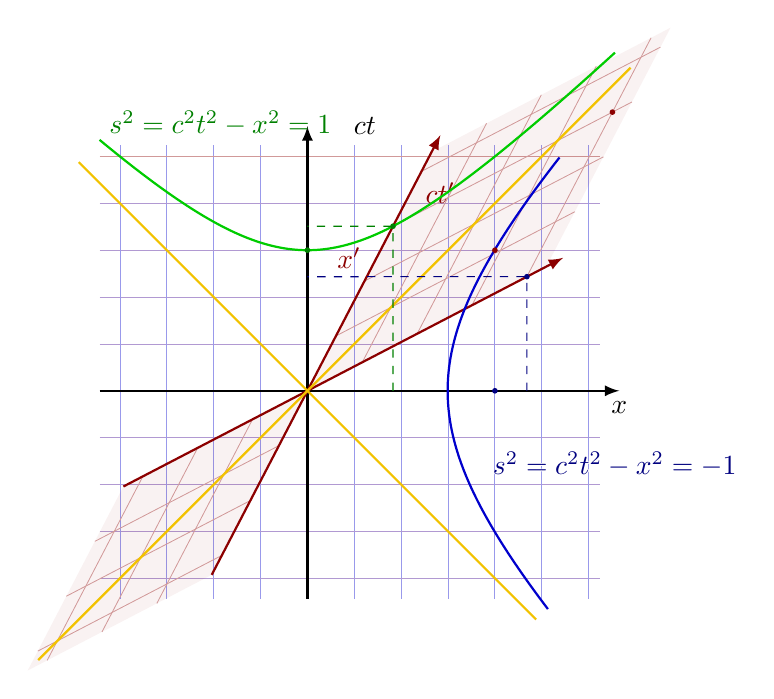
\begin{tikzpicture}[scale=1.2][!]
  \message{Invariant hyperboloids^^J}
  
  % SETTINGS
  \def\xmin{2.2}
  \def\xmax{3.1}
  \def\ymin{2.2}
  \def\ymax{2.6}
  \def\xmaxp{2.85} % maximum of rotated axis
  \def\Nlines{4} % number of world lines (at constant x/t)
  \pgfmathsetmacro\ang{atan(0.52)} % angle between x and x' axes
  \pgfmathsetmacro\d{0.64*\xmax/\Nlines} % grid size
  \pgfmathsetmacro\D{\d/cos(\ang)/sqrt(1-tan(\ang)^2)} % grid size, boosted
  \pgfmathsetmacro\dextra{(\Nlines+1)*\d} % extra line
  \pgfmathsetmacro\st{3*\d} % spacetime interval
  \pgfmathsetmacro\sx{4*\d} % spacetime interval
  \pgfmathsetmacro\sr{sqrt(\sx^2-\st^2)} % spacetime interval sr^2 = st^2 - sx^2 < 0
  \pgfmathsetmacro\Ax{3*\D*sin(\ang)} % x coordinate of event A
  \pgfmathsetmacro\Ay{3*\D*cos(\ang)} % y coordinate of event A
  \pgfmathsetmacro\Bx{4*\D*cos(\ang)} % x coordinate of event B
  \pgfmathsetmacro\By{4*\D*sin(\ang)} % y coordinate of event B
  \pgfmathsetmacro\Cx{\Ay+\By} % x coordinate of event C' %(\Bx+tan(\ang)*\Ay)/sqrt(1-tan(\ang)^2)
  \coordinate (O)  at (0,0);
  \coordinate (X)  at (\xmax+0.2,0);
  \coordinate (T)  at (0,\ymax+0.2);
  \coordinate (X') at (\ang:\xmaxp+0.2);
  \coordinate (T') at (90-\ang:\xmaxp+0.2);
  \coordinate (A)  at (0,\st);        % event A
  \coordinate (A') at (90-\ang:3*\D); % event A', boosted A
  \coordinate (B)  at (\sx,0);        % event A
  \coordinate (B') at (\ang:4*\D);    % event A', boosted A
  \coordinate (C)  at (4*\d,3*\d);    % event C
  
  % WORLD LINE GRID
  \message{  Making world lines...^^J}
  \foreach \i [evaluate={\x=\i*\d;}] in {1,...,\Nlines}{
    \message{  Running i/N=\i/\Nlines, x=\x...^^J}
    \draw[world line]   (-\x,-\ymin) -- (-\x,\ymax);
    \draw[world line]   ( \x,-\ymin) -- ( \x,\ymax);
    \draw[world line t] (-\xmin,-\x) -- (\xmax,-\x);
    \draw[world line t] (-\xmin, \x) -- (\xmax, \x);
  }
  \draw[world line]    (\dextra,-\ymin)  -- (\dextra,\ymax);
  \draw[world line]    (\dextra+\d,-\ymin) -- (\dextra+\d,\ymax);
  %\draw[world line'] (-\xmin,-\dextra) -- (\xmax,-\dextra);
  \draw[world line'] (-\xmin,\dextra) -- (\xmax,\dextra);
  
  % BOOSTED WORLD LINE GRID
  \message{  Making world lines for boosted frame...^^J}
  \fill[mydarkred,opacity=0.05]
    (O) --++ (\ang:\xmaxp) --++ (90-\ang:\xmaxp) --++ (\ang:-\xmaxp) -- cycle;
  \fill[mydarkred,opacity=0.05]
    (O) --++ (\ang:\D-\xmaxp) --++ (90-\ang:\D-\xmaxp) --++ (\ang:\xmaxp-\D) -- cycle;
  \foreach \i [evaluate={\x=\i*\D;}] in {1,...,\Nlines}{
    \message{  Running i/N=\i/\Nlines, x=\x...^^J};
    \ifnumcomp{\i}{<}{\Nlines}{
      \draw[world line'] (\ang:-\x) --++ (90-\ang:\D-\xmaxp);
      \draw[world line'] (90-\ang:-\x) --++ (\ang:\D-\xmaxp);
    }{}
    \draw[world line'] (\ang:\x) --++ (90-\ang:\xmaxp);
    \draw[world line'] (90-\ang:\x) --++ (\ang:\xmaxp);
  }
  
  % AXES
  \draw[->,thick] (0,-\ymin) -- (T) node[left=-1] {$ct$};
  \draw[->,thick] (-\xmin,0) -- (X) node[below=0] {$x$};
  \draw[->,thick,mydarkred] (90-\ang:\D-\xmaxp) -- (T')
    node[right=2,above=-1] {$ct'$};
  \draw[->,thick,mydarkred] (\ang:\D-\xmaxp) -- (X') node[below=2,right=-3] {$x'$};
  
  % LIGHTCONE
  \draw[myorange,thick]
    (-1.1*\xmin,1.1*\xmin) -- (1.1*\ymin,-1.1*\ymin)
    (-\xmaxp,-\xmaxp) -- (1.2*\xmaxp,1.2*\xmaxp);
  
  % SPACELIKE HYPERBOLOIDS
  \draw[mygreen,thick,samples=\Nsamples,smooth,variable=\x,domain=-\xmin:1.05*\xmax]
    plot(\x,{sqrt((\st)^2+(\x)^2)});
%  \draw[mydarkgreen,very thick,samples=\Nsamples,variable=\x,domain=0:\Ax,
%        decoration={markings,mark=at position 0.58 with %{\arrow{latex}}},postaction={decorate}]
%    plot(\x,{sqrt((\st)^2+(\x)^2)});
  \node[mydarkgreen,right=1,above right=0] at (-\xmin,\ymax)
    {$s^2 = c^2t^2-x^2=1$};
  
  % TIMELIKE HYPERBOLOIDS
%  \draw[myred,very thick,samples=\Nsamples,variable=\y,domain=\st:\Cx,
%        decoration={markings,mark=at position 0.58 with %{\arrow{latex}}},postaction={decorate}]
%    plot({sqrt(\sr^2+(\y)^2)},\y);
  \draw[myblue,thick,samples=\Nsamples,smooth,variable=\y,domain=-1.05*\ymin:0.95*\ymax]
    plot({sqrt(\sx^2+(\y)^2)-0.5},\y);
%  \draw[mydarkblue,very thick,samples=\Nsamples,variable=\y,domain=0:\By,
%        decoration={markings,mark=at position 0.58 with %{\arrow{latex}}},postaction={decorate}]
%    plot({sqrt(\sx^2+(\y)^2)-0.5},\y);
  \node[mydarkblue,right=0] at (0.6*\xmax,-0.25*\xmax)
    {\contour{white}{$s^2 = c^2t^2-x^2=-1$}};
  
  % TICKS
  \draw[mydarkgreen,dashed] ({\Ax},0) -- (A') -- (0,{\Ay});
  \draw[mydarkblue,dashed] ({\Bx},0) -- (B') -- (0,{\By});
%  \tick{0,\st}{0} node[mydarkgreen,right=4,below left=-2.5] {$ct_1$};
%  \tick{\sx,0}{90} node[mydarkblue,below=1,below left=-3] {$x_1$};
%  \tick{0,\Ay}{0} node[mydarkgreen,above=1,left=-2]
%    {\contour{white}{$ct_1\cosh\phi$}};
%  \tick{\Ax,0}{90} node[mydarkgreen,right=4,below=-4]
%    {\contour{white}{$ct_1\sinh\phi$}};
%  \tick{\Bx,0}{90} node[mydarkblue,right=9,below=-4]
%    {\contour{white}{$x_1\cosh\phi$}};
%  \tick{0,\By}{0} node[mydarkblue,below=1,left=-2]
%    {\contour{white}{$x_1\sinh\phi$}};
  
  % EVENTS
  \fill[mydarkgreen] (A)  circle(0.03); % event A
  \fill[mydarkgreen] (A') circle(0.03); % event A'
  \fill[mydarkblue]  (B)  circle(0.03); % event B
  \fill[mydarkblue]  (B') circle(0.03); % event B'
  \fill[mydarkred]   (C)  circle(0.03); % event C
  \fill[mydarkred] (\ang:4*\D)++(90-\ang:3*\D) coordinate (C') circle(0.03); % event C'
  %\node[mydarkred,above=2,right=6] at (C') {$\left\{\begin{aligned}
  %  ct' &= ct\cosh\phi -  x\sinh\phi \\
  %   x' &=  x\cosh\phi - ct\sinh\phi
  %\end{aligned}\right.$};
  
\end{tikzpicture}
\end{center}


\end{enumerate}


\section{Sheet 1 — Exercise 3 (Localization of relativistic particles)}
\begin{enumerate}[a)]
\item Pair production - locate particle smaller then the Compton wavelenth $\lambda_C=\hbar/mc$. Back of the envelope estimate
\begin{align}
E=\sqrt{m^2c^4+p^2c^2}\qquad&\rightarrow\Delta p\geq mc\\
\Delta x \cdot\Delta p\geq\frac{\hbar}{2}\qquad&\rightarrow\Delta x \simeq\frac{\hbar}{2mc}
\end{align}
\begin{itemize}
\item Top quark $7\cdot10^{-18}$m
\item Proton $1.3\cdot10^{-13}$m
\item Electron $2.4\cdot10^{-12}$m
\item Hydrogen $1.3\cdot10^{-13}$m
\end{itemize}

\item
\begin{itemize}
\item Top quark $\Delta x $ {\bf kind of similar} to physical size ($10^{-19}$m)
\item Proton $\Delta x $ {\bf larger} than physical size ($0.8\cdot10^{-15}$m)
\item Electron $\Delta x $ {\bf larger} than physical size of 0m (point)
\end{itemize}

\item
\begin{align}
\Delta p &\ge\frac{\hbar}{2\Delta x}\\
E_\text{part}&\ge\sqrt{m_\text{part}^2c^4+\frac{\hbar^2c^2}{4\Delta x^2}}\simeq\frac{\hbar c}{2\Delta x}
\end{align}
\end{enumerate}
\newpage

\section{Sheet 2 — Exercise 1 (Schroedinger field quantization)}
\begin{enumerate}[a)]
\item Canonical variables $\psi,\psi^*$
\begin{align}
\pi&=\frac{\partial\mathcal{L}}{\partial\dot{\psi}}=i\psi^*\\
\pi^*&=\frac{\partial\mathcal{L}}{\partial\dot{\psi^*}}=0\qquad \text{(constraint)}
\end{align}
Then
\begin{align}
\mathcal{H}
&=\pi\dot\psi+\pi^*\dot\psi^*-\mathcal{L}\\
&=\frac{1}{2m}(\nabla\psi^*)(\nabla\psi)+V\psi^*\psi\\
&=-\frac{i}{2m}(\nabla\pi)(\nabla\psi)-iV\pi\psi\\
H&=-i\int d^3x \left(\frac{1}{2m}(\nabla_x\pi(x))(\nabla_x\psi(x))+V\pi(x)\psi(x)\right)\\
&=-i\int d^3x \left(-\frac{1}{2m}\pi(x)(\triangle_x\psi(x))+V\pi(x)\psi(x)\right)
\end{align}
Using the standard commutators
\begin{align}
[\psi(x),\pi(y)]=i\delta^{(3)}(x-y),\qquad
[\psi(x),\psi(y)]=0,\qquad
[\pi(x),\pi(y)]=0
\end{align}
Heisenberg equations: when we integrate by parts to move the $\nabla,\triangle$ we assume well behaving boundaries
\begin{align}
i\partial_t\psi(y)
&=[H,\psi(y)]\\
&=i\int d^3x \frac{1}{2m}\pi(x)(\triangle_x\psi(x))\psi(y)-\frac{1}{2m}\psi(y)\pi(x)(\triangle_x\psi(x))-V(x)\pi(x)\psi(x)\psi(y)+V(x)\psi(y)\pi(x)\psi(x)\\
&=i\int d^3x \frac{1}{2m}\pi(x)(\triangle_x\psi(x))\psi(y)-\frac{1}{2m}(\pi(x)\psi(y)-i\delta^{(3)}(x-y))(\triangle_x\psi(x))\\
&\qquad\qquad\qquad-V(x)\pi(x)\psi(x)\psi(y)+V(x)(\pi(x)\psi(y)-i\delta^{(3)}(x-y))\psi(x)\\
&=i\int d^3x -\frac{1}{2m}(-i\delta^{(3)}(x-y))(\triangle_x\psi(x))-V(-i\delta^{(3)}(x-y))\psi(x)\\
&=-\int d^3x \frac{1}{2m}\delta^{(3)}(x-y)(\triangle_x\psi(x))-V(x)\delta^{(3)}(x-y)\psi(x)\\
&=-\frac{1}{2m}\triangle_y\psi(y)+V(y)\psi(y)
\end{align}
which looks like the one particle Schroedinger equation.
\begin{align}
i\partial_t\pi(y)
&=[H,\pi(y)]\\
&=i\int d^3x\frac{1}{2m}\left(\pi(x)\triangle_x\psi(x)\pi(y)-\pi(y)\pi(x)\triangle_x\psi(x)\right) -V\pi(x)i\delta^{(3)}(x-y)\\
&=i\int d^3x\frac{1}{2m}\left(\pi(x)\triangle_x(\pi(y)\psi(x)+i\delta^{(3)}(x-y))-\pi(y)\pi(x)\triangle_x\psi(x)\right) -V\pi(x)i\delta^{(3)}(x-y)\\
&=i\int d^3x\frac{1}{2m}i\pi(x)\triangle_x\delta^{(3)}(x-y)-\frac{1}{2m}\pi(x)\pi(y)\triangle_x\psi(x) -V\pi(x)i\delta^{(3)}(x-y)\\
&=i\int d^3x\frac{1}{2m}i\pi(x)\triangle_x\delta^{(3)}(x-y)-\frac{1}{2m}\pi(x)\triangle_x\pi(y)\psi(x) -V\pi(x)i\delta^{(3)}(x-y)\\
&=i\int d^3x\frac{1}{2m}i\triangle_x\pi(x)\delta^{(3)}(x-y) -V\pi(x)i\delta^{(3)}(x-y)\\
&=-\frac{1}{2m}\triangle_y\pi(y) +V(y)\pi(y)
\end{align}
which with $\pi=i\psi^*$ gives the complex conjugated SG
\begin{align}
-i\partial_t\psi^*=-\frac{1}{2m}\triangle\psi^*+V\psi^*
\end{align}
\item With
\begin{align}
H&=-i\int d^3x \left(-\frac{1}{2m}\pi(x)(\triangle_x\psi(x))+V(x)\pi(x)\psi(x)\right)
\end{align}
and the usual definition of the field-theory Poisson bracket
\begin{align}
\{H,\psi(x)\}
&=\int d^3y\left(\frac{\partial H}{\partial\psi(y)}\frac{\partial\psi(x)}{\partial\pi(y)}
\textcolor{blue}{-\frac{\partial H}{\partial\pi(y)}\frac{\partial\psi(x)}{\partial\psi(y)}}\right)+
\left(\frac{\partial H}{\partial\psi^*(y)}\frac{\partial\psi(x)}{\partial\pi^*(y)}
-\frac{\partial H}{\partial\pi^*(y)}\frac{\partial\psi(x)}{\partial\psi^*(y)}\right)\\
&=-i\int d^3y\int d^3x (-1)\left(-\frac{1}{2m}\triangle_x\psi(x)+V(x)\psi(x)\right)\delta^{(3)}(x-y)\cdot\delta^{(3)}(x-y)\\
&=i\int d^3y \left(-\frac{1}{2m}\triangle_y\psi(y)+V(y)\psi(y)\right)\delta^{(3)}(x-y)\\
&=i\left(-\frac{1}{2m}\triangle_y\psi(y)+V(y)\psi(y)\right)
\end{align}
and with $\dot{\psi}=\{H,\psi(x)\}$ we recover the Schroedinger equation.

Just out of curiosity we calculate two more Poisson brackets ($\pi=i\psi^*$)
\begin{align}
\{\psi(x),\psi(y)\}
&=\int d^3z\left(\frac{\partial\psi(x)}{\partial\psi(z)}\frac{\partial\psi(y)}{\partial\pi(z)}
-\frac{\partial\psi(x)}{\partial\pi(z)}\frac{\partial\psi(y)}{\partial\psi(z)}\right)+
\left(\frac{\partial\psi(x)}{\partial\psi^*(z)}\frac{\partial\psi(y)}{\partial\pi^*(z)}
-\frac{\partial\psi(x)}{\partial\pi^*(z)}\frac{\partial\psi(y)}{\partial\psi^*(z)}\right)\\
&=0\\
\{\psi(x),\pi(y)\}
&=\int d^3z\left(\textcolor{blue}{\frac{\partial\psi(x)}{\partial\psi(z)}\frac{\partial\pi(y)}{\partial\pi(z)}}
-\frac{\partial\psi(x)}{\partial\pi(z)}\frac{\partial\pi(y)}{\partial\psi(z)}\right)+
\left(\frac{\partial\psi(x)}{\partial\psi^*(z)}\frac{\partial\pi(y)}{\partial\pi^*(z)}
-\frac{\partial\psi(x)}{\partial\pi^*(z)}\frac{\partial\pi(y)}{\partial\psi^*(z)}\right)\\
&=\int d^3z\delta^{(3)}(x-z)\delta^{(3)}(y-z)\\
&=\delta^{(3)}(x-z)
\end{align}

\item As $\psi$ and $\psi^*$ all terms appear as some kind of product we try a global gauge transformation of (same idea as for complex KG field)
\begin{align}
\psi\rightarrow e^{i\varepsilon}\psi&\simeq(1+i\varepsilon)\psi=\psi+i\varepsilon\psi\\
\psi^*\rightarrow e^{-i\varepsilon}\psi^*&\simeq(1-i\varepsilon)\psi^*=\psi^*-i\varepsilon\psi^*
\end{align}
so $\delta\psi=i\varepsilon\psi$ and $\delta\psi^*=-i\varepsilon\psi^*$.

Then we look at the three terms of the Lagrangian separately
\begin{align}
\psi^*\dot{\psi}\rightarrow (\psi^*-i\varepsilon\psi^*)(\dot{\psi}+i\varepsilon\dot{\psi})
&=\psi^*\dot{\psi}+i\varepsilon(-\psi^*\dot{\psi}+\psi^*\dot{\psi})+\mathcal{O}(\varepsilon^2)\\
&=\psi^*\dot{\psi}\\
&\rightarrow\delta(\psi^*\dot{\psi})=0
\end{align}
second term
\begin{align}
(\nabla\psi^*)\nabla(\psi)\rightarrow (\nabla\psi^*-i\varepsilon\psi^*)\nabla(\psi+i\varepsilon\psi)
&=(\nabla\psi^*)(\nabla\psi)+i\varepsilon((\nabla\psi^*)(\nabla\psi)-(\nabla\psi^*)(\nabla\psi))+\mathcal{O}(\varepsilon^2)\\
&=(\nabla\psi^*)(\nabla\psi)\\
&\rightarrow\delta((\nabla\psi^*)(\nabla\psi))=0
\end{align}
and third term
\begin{align}
\psi^*{\psi}\rightarrow (\psi^*-i\varepsilon\psi^*)({\psi}+i\varepsilon{\psi})
&=\psi^*{\psi}+i\varepsilon(-\psi^*{\psi}+\psi^*{\psi})+\mathcal{O}(\varepsilon^2)\\
&=\psi^*{\psi}\\
&\rightarrow\delta(\psi^*{\psi})=0.
\end{align}
So we conclude that the Lagrangian is invariant under this transformation. Then
\begin{align}
j^\mu
&=\frac{\partial\mathcal{L}}{\partial(\partial_\mu\psi)}\delta\psi
+\frac{\partial\mathcal{L}}{\partial(\partial_\mu\psi^*)}\delta\psi^*\\
j^0&=i\psi^*(i\varepsilon\psi)\\
&=-\varepsilon\psi^*\psi\\
j^m&=-\frac{1}{2m}\left((\nabla\psi^*)(i\varepsilon\psi)+(\nabla\psi)(-i\varepsilon\psi^*)\right)\\
&=-\frac{i\varepsilon}{2m}\left((\nabla\psi^*)\psi-(\nabla\psi)\psi^*\right)
\end{align}
and 
\begin{align}
Q&=\int d^3x\;j^0=-\varepsilon\int d^3x\;\psi^*\psi.
\end{align}
The charge operator becomes then (we are cheating a bit because we no idea about the operator ordering)
\begin{align}
\hat{Q}
&=-\varepsilon\int d^3x\,\hat{\psi}^\dagger(x)\hat{\psi}(x)
=-\varepsilon\int d^3x
\int\frac{d^3p}{(2\pi)^{3/2}}e^{-ipx}a^\dagger_p
\int\frac{d^3q}{(2\pi)^{3/2}}e^{iqx}a_q\\
&=\varepsilon\int\frac{d^3p}{(2\pi)^{3/2}}\int\frac{d^3q}{(2\pi)^{3/2}}a^\dagger_pa_q \int d^3x\,e^{i(q-p)x}\\
&=\varepsilon\int\frac{d^3p}{(2\pi)^{3/2}}\int\frac{d^3q}{(2\pi)^{3/2}}a^\dagger_pa_q\;(2\pi)^3\delta^{(3)}(q-p)\\
&=\varepsilon\int d^3p\,a^\dagger_p a_q
\end{align}

\item As we recover the non-relativistic Schroedinger theory there are no anti-particles - so there is only one charge amount associated with a particle - so particle and charge conservation are identical.

In a relativistic theory with particles always come with anti-particles. In case the particles have charge $q$ then the anti-particles have charge $-q$. If a particle - anti-particle pair is created - the total charge will be conserved but the particle number is not. 

\item The canonical approach starting with a field theory is to calculate the energy momentum tensor and derive the momentum from the $T^{0k}$ components. So we start with the definition (with metric  signature diag $\eta=(1,-1,-1,-1)$)
\begin{align}
T^{\mu\nu}
&=\frac{\partial\mathcal{L}}{\partial(\partial_\mu\psi)}(\partial^\nu\psi)
+\frac{\partial\mathcal{L}}{\partial(\partial_\mu\psi^*)}(\partial^\nu\psi^*)-\mathcal{L}\eta^{\mu\nu}\\
&=\frac{\partial\mathcal{L}}{\partial(\partial_\mu\psi)}(\eta^{\nu\alpha}\partial_\alpha\psi)
+\frac{\partial\mathcal{L}}{\partial(\partial_\mu\psi^*)}(\eta^{\nu\alpha}\partial_\alpha\psi^*)-\mathcal{L}\eta^{\mu\nu}
\end{align}
To sense check we calculate the $T^{00}$ component first 
\begin{align}
T^{00}
&=i\psi^*\dot{\psi}+0-i\psi^*\dot{\psi}+\frac{1}{2m}|\nabla_x\psi(x)|^2+V(x)|\psi(x)|^2\\
&=\frac{1}{2m}|\nabla_x\psi(x)|^2+V(x)|\psi(x)|^2
\end{align}
and see that we recover the Hamiltonian density from (a). So we continue
\begin{align}
T^{0k}
&=i\psi^*(-\partial_k\psi)\\
P^k&=-i\int d^3x\; \psi^*(\partial_k\psi)
\end{align}
The (guessing the operator ordering)
\begin{align}
\hat{P}^k
&=-i\int d^3x
\int\frac{d^3p}{(2\pi)^{3/2}}e^{-ipx}a^\dagger_p
\int\frac{d^3q}{(2\pi)^{3/2}}(\partial_k e^{iqx})a_q\\
&=-i
\int\frac{d^3p}{(2\pi)^{3/2}}
\int\frac{d^3q}{(2\pi)^{3/2}}(iq_k)a^\dagger_pa_q\int d^3x\,e^{i(q-p)x}\\
&=
\int\frac{d^3p}{(2\pi)^{3/2}}
\int\frac{d^3q}{(2\pi)^{3/2}}q_k\,a^\dagger_pa_q(2\pi)^3\delta^{(3)}(q-p)\\
&=\int d^3p\,p_k\,a^\dagger_pa_q
\end{align}

\end{enumerate}
\newpage

\section{Sheet 3 — Exercise 1 (Poincare representations on fields)}
\begin{enumerate}[a)]
\item The representation is $f'(x')=f'(\Lambda x+a)=f(x)$. 

Now lets check the result for Alice with the definitions
\begin{align}
f'(\Lambda x+a)&=f(x)\\
f'(x)&=f(\Lambda^{-1}(x-a))\\
U(\Lambda,a)f(x)&=f'(x)\\
&=f(\Lambda^{-1}(x-a))\\
&=f(\Lambda^{-1}x-\Lambda^{-1}a)
\end{align}
we calculate (evaluating left operator first!!!)
\begin{align}
U(\Lambda_2,a_2)U(\Lambda_1,a_1)f(x)
&=U(\Lambda_2,a_2)(U(\Lambda_1,a_1)f(x))\\
&=(U(\Lambda_1,a_1)f)(\Lambda_2^{-1}(x-a_2))\\
&=f(\Lambda_1^{-1}((\Lambda_2^{-1}x-\Lambda_2^{-1}a_2)-a_1))\\
&=f(\Lambda_1^{-1}\Lambda_2^{-1}x-\Lambda_1^{-1}\Lambda_2^{-1}a_2-\Lambda_1^{-1}a_1)
\end{align}
and
\begin{align}
U(\Lambda_2\Lambda_1,\Lambda_2a_1+a_2)f(x)
&=f((\Lambda_2\Lambda_1)^{-1}(x-\Lambda_2a_1-a_2))\\
&=f(\Lambda_1^{-1}\Lambda_2^{-1}(x-\Lambda_2a_1-a_2))\\
&=f(\Lambda_1^{-1}\Lambda_2^{-1}x-\Lambda_1^{-1}a_1-\Lambda_1^{-1}\Lambda_2^{-1}a_2)
\end{align}
I think the confusing point here is the notation of the order of the operations - $U(\Lambda_2,a_2)U(\Lambda_1,a_1)$ acting on $f(x)$. We used
\begin{align}
x'&=\Lambda_1 x + a_1\\
x''&=\Lambda_2(\Lambda_1 x + a_1)+a_2\\
&=\Lambda_2\Lambda_1 x + \Lambda_2a_1+a_2\\
\rightarrow(\Lambda_2,a_2)\circ(\Lambda_1,a_1)&=(\Lambda_2\Lambda_1,\Lambda_2a_1+a_2)\\
\rightarrow U(\Lambda_2,a_2)U(\Lambda_1,a_1)
&=U((\Lambda_2,a_2)\circ(\Lambda_1,a_1))\\
&=U(\Lambda_2\Lambda_1,\Lambda_2a_1+a_2)
\end{align}


\item Poincare transformation for spacetime-independent objects 
\begin{align}
U(\Lambda,a)&=e^{ia_\mu P^\mu}e^{-\frac{i}{2}\omega_{\mu\nu} J^{\mu\nu}}\\
&\simeq1+ia_\mu {P}^\mu-\frac{i}{2}\omega_{\rho\sigma}{J}^{\rho\sigma}
\end{align}
and for spacetime-dependent objects (generators are now operators) - so we have infinite dimensional representations
\begin{align}
U(\delta+\omega,a)
&=1+ia_\mu \hat{P}^\mu-\frac{i}{2}\omega_{\rho\sigma}\hat{J}^{\rho\sigma}
\end{align}
We see that there are two sets of generators: Lorentz transformations and translations

With $\Lambda^\alpha_{\;\mu}\approx\delta^\alpha_\mu+\omega^\alpha_{\;\;\mu}$ we obtain for the infinitesimal Poincare transformation
\begin{align}
x'^\mu
&=\Lambda^\mu_{\;\alpha}x^\alpha+a^\mu\\
&\simeq\left(\delta^\mu_\alpha+\omega^\mu_{\;\;\alpha}\right)x^\alpha+a^\mu\\
&\simeq x^\mu+\omega^\mu_{\;\;\alpha}x^\alpha+a^\mu.
\end{align}
The inverted PT is then given by
\begin{align}
x&=\Lambda^{-1}(x'-a)\\
&=\Lambda^{-1}x'-\Lambda^{-1}a\\
x^\mu&\simeq\left(\delta^\mu_\alpha-\omega^\mu_{\;\;\alpha}\right)x'^\alpha-\left(\delta^\mu_\alpha-\omega^\mu_{\;\;\alpha}\right)a^\alpha\\
&\simeq x'^\mu-\omega^\mu_{\;\;\alpha}x'^\omega-a^\mu+\mathcal{O}(\epsilon\cdot a)
\end{align}
Because of 
\begin{align}
\phi'(x')=\left(1+ia_\mu\hat{P}^\mu-\frac{i}{2}\omega_{\rho\sigma}\hat{J}^{\rho\sigma}\right)\phi(x)
\end{align}
and
\begin{align}
\phi'(x')=\phi(x)
&\quad\Leftrightarrow\quad\phi'(\Lambda x+a)=\phi(x)\\
&\quad\Leftrightarrow\quad\phi'(x)=\phi(\Lambda^{-1}(x-a))
\end{align}
we can now calculate 
\begin{align}
\delta\phi(x)
&\equiv\phi'(x)-\phi(x)\\
&=\phi(\Lambda^{-1}(x-a))-\phi(x)\\
&\simeq\phi(x^\mu-\omega^\mu_{\;\;\alpha}x^\alpha-a^\mu)-\phi(x)\\
&\simeq\phi(x)+\partial_\mu\phi(x)\cdot(-\omega^\mu_{\;\;\alpha}x^\alpha-a^\mu)-\phi(x)\\
&\simeq-(a^\mu+\omega^\mu_{\;\;\alpha}x^\alpha)\partial_\mu\phi(x)\\
&\simeq-(a^\mu+\omega^{\mu\alpha}x_\alpha)\partial_\mu\phi(x)\\
&\simeq-\left(a^\mu+\frac{1}{2}\left(\omega^{\mu\alpha}-\omega^{\alpha\mu}\right)x_\alpha\right)\partial_\mu\phi(x)\\
&\simeq-\left(a^\mu\partial_\mu+\frac{1}{2}\left(\omega^{\mu\alpha}x_\alpha\partial_\mu-\omega^{\alpha\mu}x_\alpha\partial_\mu\right)\right)\phi(x)\\
&\simeq-\left(a^\mu\partial_\mu+\frac{1}{2}\left(\omega^{\mu\alpha}x_\alpha\partial_\mu-\omega^{\mu\alpha}x_\mu\partial_\alpha\right)\right)\phi(x)\\
&\simeq i\left(a^\mu i\partial_\mu+\frac{1}{2}\omega^{\mu\alpha}i\left(x_\alpha\partial_\mu-x_\mu\partial_\alpha\right)\right)\phi(x)\\
&\simeq i\left(a^\mu i\partial_\mu-\frac{1}{2}\omega^{\mu\alpha}i\left(x_\mu\partial_\alpha-x_\alpha\partial_\mu\right)\right)\phi(x)\\
&\simeq i\left(a^\mu \hat{P}_\mu-\frac{1}{2}\omega^{\mu\alpha}\hat{J}_{\mu\alpha}\right)\phi(x)
\end{align}
So the scalar field representation is given by
\begin{align}
\hat{P}_\mu&=i\partial_\mu\\
\hat{J}_{\mu\nu}&=i(x_\mu\partial_\nu-x_\nu\partial_\mu)
\end{align}
\end{enumerate}

\section{Sheet 3 — Exercise 2 (Poincare representations on quantum fields)}
Adam looks right
\begin{align}
U(\Lambda_1,a_1)^{-1}\psi_A(\Lambda_1 x+a_1)U(\Lambda_1,a_1)
&=D_{AB}(\Lambda_1)\psi_B(x)\\
U(\Lambda_1,a_1)^{-1}\psi_A(x)U(\Lambda_1,a_1)
&=D_{AB}(\Lambda_1)\psi_B(\Lambda_1^{-1}(x-a_1))
\end{align}
The combined transformation ($\sim\Lambda_1\Lambda_2$) looks like
\begin{align}
U(\Lambda_1\Lambda_2,\Lambda_1a_2+a_1)^{-1}\psi_A(\Lambda_1 x+a_1)U(\Lambda_1\Lambda_2,\Lambda_1a_2+a_1)&=D_{AC}(\Lambda_1\Lambda_2)\psi_C(\Lambda_2^{-1}(x-a_1))
\end{align}
With $U((\Lambda_1,a_1)(\Lambda_2,a_2))^{-1}=U(\Lambda_2,a_2)^{-1}U(\Lambda_1,a_1)^{-1}$ we calculate
\begin{align}
U(\Lambda_2,a_2)^{-1}\underbrace{U(\Lambda_1,a_1)^{-1}\psi_A(\Lambda_1 x+a_1)U(\Lambda_1,a_1)}_{=D_{AB}(\Lambda_1)\psi_B(x)}U(\Lambda_2,a_2)
&=D_{AB}(\Lambda_1)U(\Lambda_2,a_2)^{-1}\psi_B(x)U(\Lambda_2,a_2)\\
&=D_{AB}(\Lambda_1)D_{BC}(\Lambda_2)\psi_C(\Lambda_2^{-1}(x-a_2))
\end{align}
which completes the proof.



\section{Sheet 3 — Exercise 3 (Pauli-Lubanski operator)}
\begin{enumerate}[a)]
\item Using the definition of the angular momentum $J_i=\frac{1}{2}\epsilon_{ijk}J^{jk}$
\begin{align}
W_\mu
&=\frac{1}{2}\epsilon_{\mu0\rho\sigma}P^0J^{\rho\sigma}\qquad\rightarrow\qquad W=(0,\mathbf{W})\\
W_0&=0\\
W_1&=\frac{m}{2}\left(
\epsilon_{1023}J^{23}
+\epsilon_{1032}J^{32}
\right)
=\frac{m}{2}\left(-J^{23}+J^{32}\right)=mJ_1\\
W_2&=\frac{m}{2}\left(
\epsilon_{2031}J^{31}
+\epsilon_{2013}J^{13}
\right)
=\frac{m}{2}\left(-J^{13}+J^{31}\right)=mJ_2\\
W_3&=\frac{m}{2}\left(
\epsilon_{3012}J^{12}
+\epsilon_{3021}J^{21}
\right)
=\frac{m}{2}\left(J^{12}-J^{21}\right)=mJ_3
\end{align}
\item Using the result from a) and the definition of the boosts $K_i=J^{i0}$
\begin{align}
W_\mu
&=\frac{1}{2}\epsilon_{\mu0\rho\sigma}P^0J^{\rho\sigma}+
\frac{1}{2}\epsilon_{\mu3\rho\sigma}P^3J^{\rho\sigma}\\
W_0
&=0+\frac{k}{2}(\epsilon_{0312}J^{12}+\epsilon_{0321}J^{21})
=\frac{k}{2}(J^{12}-J^{21})
=kJ_3\\
W_1
&=kJ_1+\frac{k}{2}(\epsilon_{1320}J^{20}+\epsilon_{1302}J^{02})
=kJ_1+\frac{k}{2}(J^{20}-J^{02})
=k(J_1+K_2)\\
W_2
&=kJ_2+\frac{k}{2}(\epsilon_{2310}J^{10}+\epsilon_{2301}J^{01})
=kJ_2+\frac{k}{2}(-J^{10}+J^{01})
=k(J_2-K_1)\\
W_3
&=kJ_3+0
=kJ_3
\end{align}

\item With the Lorentz algebra
\begin{align}
[J^i,J^j]=i\epsilon_{ijk}J^k\\
[J^i,K^j]=i\epsilon_{ijk}K^k\\
[K^i,K^j]=-i\epsilon_{ijk}J^k\\
\end{align}
we calculate
\begin{align}
[A,B]=[W_2,W_1] 
&= k^2[J_2-K_1,J_1+K_2]\\
&=k^2([J_2,J_1]-[K_1,J_1]+[J_2,K_2]-[K_1,K_2])\\
&= k^2((-iJ_3)-0+0-(-iJ_3))\\
&=0\\
[J_z,A]=[J_3,W_2]
&=k[J_3,(J_2-K_1)]\\
&=k[J_3,J_2]-[J_3,K_1)]\\
&=k(-iJ_1-(iK_2))\\
&=-ik(J_1+K_2)\\
&=-iW_1
\end{align}
\end{enumerate}
\newpage

\section{Sheet 4 — Exercise 1 (Noether Theorem)}

\begin{enumerate}[a)]
\item With
\begin{align}
x'^{\rho}
&=\Lambda^\rho_{\;\sigma} x^\sigma+a^\rho\\
&=(\delta^\rho_{\;\sigma}+\omega^\rho_{\;\sigma}) x^\sigma+a^\rho\\
D(\Lambda)_{AB}
&\simeq 1-\frac{i}{2}\omega_{\rho\sigma}(S^{\rho\sigma})_{AB}\\
\phi_A(x)\rightarrow\phi_A'(x)&=D_{AB}(\Lambda)\phi_B(\Lambda^{-1}(x-a))
\end{align}
then
\begin{align}
\delta\phi_A(x)
&\equiv D_{AB}(\Lambda)\phi_B(\Lambda^{-1}(x-a))-\phi_B(x)\\
&\simeq \left[1-\frac{i}{2}\omega_{\rho\sigma}(S^{\rho\sigma})_{AB}\right]\phi_B\left((1-\omega^\rho_{\;\sigma})(x^\sigma-a^\sigma)\right)-\phi_B(x)\\
&\simeq \left[1-\frac{i}{2}\omega_{\rho\sigma}(S^{\rho\sigma})_{AB}\right]\phi_B\left(x^\rho-a^\rho -\omega^\rho_{\;\sigma}x^\sigma\right)-\phi_B(x)\\
&\simeq \left[1-\frac{i}{2}\omega_{\rho\sigma}(S^{\rho\sigma})_{AB}\right]\left[\phi_B(x)+\partial_\rho\phi_B(x)\cdot\left(a^\sigma +\omega^\rho_{\;\sigma}x^\sigma\right)\right]-\phi_B(x)\\
&\simeq \phi_B(x)-\frac{i}{2}\omega_{\rho\sigma}(S^{\rho\sigma})_{AB}\phi_B(x)+\left(a^\sigma +\omega^\rho_{\;\sigma}x^\sigma\right)\cdot\partial_\rho\phi_B(x)-\phi_B(x)\\
&\simeq \left(+ia_\mu P^\mu -\frac{i}{2}\omega_{\rho\sigma}J^{\rho\sigma}\right)\phi_B(x)-\frac{i}{2}\omega_{\rho\sigma}(S^{\rho\sigma})_{AB}\phi_B(x)
\end{align}
were we used the results from Problem 3.1b in the last step.

\item
Noether theorem
\begin{enumerate}[(i)]
\item Infinitesimal field transformation (same space-time point)
\begin{align}
\phi_i(x)\rightarrow\phi'_i(x)&=\phi_i(x)+\delta\phi_i(x)
\end{align}
\item Assume symmetry of the action (Lagrangian can differ by a 4-divergence)
\begin{align}
S&\rightarrow S\\
\mathcal{L}&\rightarrow\mathcal{L}+\partial_\rho X^\rho\\
\end{align}
\item alternatively
\begin{align}
\mathcal{L}
&\rightarrow\mathcal{L}(\phi_i+\delta\phi,\partial_\rho\phi_i+\delta\partial_\rho\phi_i)\\
&\rightarrow\mathcal{L}(\phi_i,\partial_\rho\phi_i)
+\frac{\partial\mathcal{L}}{\partial\phi_i}\delta\phi_i
+\frac{\partial\mathcal{L}}{\partial(\partial_\rho\phi_i)}\delta(\partial_\rho\phi_i)\\
&\rightarrow\mathcal{L}(\phi_i,\partial_\rho\phi_i)
+\partial_\rho
\left(\frac{\partial\mathcal{L}}{\partial(\partial_\rho\phi_i)}\right)\delta\phi_i
+\frac{\partial\mathcal{L}}{\partial(\partial_\rho\phi_i)}\partial_\rho(\delta\phi_i)\\
&\rightarrow\mathcal{L}(\phi_i,\partial_\rho\phi_i)
+\partial_\rho
\left(\frac{\partial\mathcal{L}}{\partial(\partial_\rho\phi_i)}\delta\phi_i\right)
\end{align}
\item compare terms to get Noether currents 
\begin{align}
j^\rho
=\frac{\partial\mathcal{L}}{\partial(\partial_\rho\phi_i)}\delta\phi_i-X^\rho
\quad\rightarrow\quad
\partial_\rho j^\rho=0
\end{align}
\item conserved quantity
\begin{align}
Q
&=\int d^3x\; j^0\\
&=\int d^3x\,\frac{\partial\mathcal{L}}{\partial(\partial_0\phi_i)}\delta\phi_i-X^0\quad\rightarrow\quad\frac{d}{dt}Q=0
\end{align}
\end{enumerate}
Now application of Poincare symmetry to scalar field
\begin{align}
x'^\mu&=\Lambda^\mu_{\;\nu} x^\nu+a^\mu\\
&\rightarrow x'^\mu\simeq(\delta^\mu_\nu+\omega^\mu_{\;\nu})x^\nu+a^\mu\\
&\rightarrow x'^\mu\simeq x^\mu+\omega^\mu_{\;\nu}x^\nu+a^\mu\\
\phi_i'(x')&=\phi_i(x)\\
&\rightarrow\phi_i'(x)=\phi(\Lambda^{-1}(x-a))\\
&\rightarrow\phi_i'(x)\simeq\phi_i((1-\omega)(x-a))\\
&\rightarrow\phi_i'(x)\simeq\phi_i(x-\omega x-a))\\
&\rightarrow\phi_i'(x)\simeq\phi_i(x)-(\omega^\mu_{\;\nu} x^\nu)\partial_\mu\phi_i(x)-a^\mu(\partial_\mu\phi_i(x))\\
&\rightarrow\delta\phi_i=-(\omega^\mu_{\;\nu} x^\nu)\partial_\mu\phi_i(x)-a^\mu(\partial_\mu\phi_i(x))\\
\mathcal{L}'(\Lambda x+a)&=\mathcal{L}(x)\\
&\rightarrow\delta\mathcal{L}=-(\omega^\mu_{\;\nu} x^\nu)\partial_\mu\mathcal{L}-a^\mu(\partial_\mu\mathcal{L})\\
&\rightarrow\delta\mathcal{L}=\partial_\mu(-\omega^\mu_{\;\nu} x^\nu\mathcal{L}-a^\mu \mathcal{L})\\
&=\textcolor{blue}{-\omega^\mu_{\;\nu} (\partial_\mu x^\nu)\mathcal{L}-\omega^\mu_{\;\nu}x^\nu \partial_\mu\mathcal{L}-a^\mu \partial_\mu\mathcal{L}}\\
&=\textcolor{blue}{-\omega^\mu_{\;\nu} \delta_\mu^\nu\mathcal{L}-\omega^\mu_{\;\nu}x^\nu \partial_\mu\mathcal{L}-a^\mu \partial_\mu\mathcal{L}}\\
&=\textcolor{blue}{-\underbrace{\omega^\mu_{\;\mu}}_{=0}\mathcal{L}-\omega^\mu_{\;\nu}x^\nu \partial_\mu\mathcal{L}-a^\mu \partial_\mu\mathcal{L}}\\
&\rightarrow X^\mu=-\omega^\mu_{\;\nu} x^\nu\mathcal{L}-a^\mu \mathcal{L}\\
\end{align}
then
\begin{align}
j^\rho
&=\frac{\partial\mathcal{L}}{\partial(\partial_\rho\phi_i)}\delta\phi_i-X^\rho\\
&=-\frac{\partial\mathcal{L}}{\partial(\partial_\rho\phi_i)}(\partial_\mu\phi_i)(\omega^\mu_{\;\nu} x^\nu+a^\mu)+\omega^\rho_{\;\nu} x^\nu\mathcal{L}+a^\rho \mathcal{L}\\
&=\left[\frac{\partial\mathcal{L}}{\partial(\partial_\rho\phi_i)}(\partial^\mu\phi_i) x^\nu-\eta^{\rho\mu} x^\nu\mathcal{L}\right]\omega_{\mu\nu}+\left[\frac{\partial\mathcal{L}}{\partial(\partial_\rho\phi_i)}(\partial_\mu\phi_i)-\eta^\mu_{\;\rho}\mathcal{L}\right](-a^\rho)
\end{align}
and we define the Energy momentum tensor
\begin{align}
T^{\rho\mu}\equiv\frac{\partial\mathcal{L}}{\partial(\partial_\rho\phi_i)}(\partial^\mu\phi_i)-\eta^{\mu\rho}\mathcal{L}
\end{align}
and the Angular momentum density
\begin{align}
\mathcal{M}^{\rho\mu\nu}
&\equiv
-\frac{\partial\mathcal{L}}{\partial(\partial_\rho\phi_i)}(\partial^\mu\phi_i) x^\nu
+\frac{\partial\mathcal{L}}{\partial(\partial_\rho\phi_i)}(\partial^\nu\phi_i) x^\mu
+\eta^{\rho\mu} x^\nu\mathcal{L}
-\eta^{\rho\nu} x^\mu\mathcal{L}\\
&=T^{\rho\nu}x^\mu-T^{\rho\mu}x^\nu
\end{align}

\item Conserved quantities
\begin{align}
P^\mu
&=\int d^3 x T^{0\mu}\\
&=\int d^3 x \frac{\partial\mathcal{L}}{\partial\dot{\phi}_i}(\partial^\mu\phi_i)-\eta^{\mu0}\mathcal{L}\\
J^{\mu\nu}&=\int d^3 x \mathcal{M}^{0\mu\nu}\\
&=\int d^3 x (T^{0\nu}x^\mu-T^{0\mu}x^\nu)
\end{align}

\end{enumerate}

\section{Sheet 4 — Exercise 2 (Quantization of spin 0 field)}
\begin{enumerate}[a)]
\item We select the scalar Klein-Gordon field with $\phi=\phi(\mathbf{x},t)$
\begin{align}
\mathcal{L}(\phi,\partial\phi)&=\frac{1}{2}g^{\mu\nu}\partial_\nu\phi\partial_\mu\phi-\frac{m^2}{2}\phi^2
\end{align}
Euler Lagrange
\begin{align}
0&=\partial_\rho\left(\frac{\partial\mathcal{L}}{\partial(\partial_\rho\phi)}\right)-\frac{\partial\mathcal{L}}{\partial\phi}\\
&\rightarrow \frac{1}{2}\partial_\rho g^{\mu\nu}(\partial_\mu\phi\delta^\rho_\nu+\partial_\nu\phi\delta^\rho_\mu)+m^2\phi=0\\
&\rightarrow \frac{1}{2}\partial_\rho(\partial^\nu\phi\delta^\rho_\nu+\partial^\mu\phi\delta^\rho_\mu)+m^2\phi=0\\
&\rightarrow \partial_\rho\partial^\rho\phi+m^2\phi=0
\end{align}
Conjugated momentum
\begin{align}
\pi(\mathbf{x},t)&=\frac{\partial\mathcal{L}}{\partial\dot{\phi}}\\
&\rightarrow \pi=\frac{1}{2}g^{00}(2\dot{\phi})\\
&\rightarrow \pi=\dot{\phi}
\end{align}
Hamilton density
\begin{align}
\mathcal{H}&=\pi\dot{\phi}-\mathcal{L}\\
&\rightarrow\mathcal{H}=\pi^2-\frac{1}{2}\pi^2+\frac{1}{2}(\nabla\phi)^2+\frac{m^2}{2}\phi^2\\
&\rightarrow\mathcal{H}=\frac{1}{2}\pi^2+\frac{1}{2}(\nabla\phi)^2+\frac{m^2}{2}\phi^2
\end{align}
Hamiltonian
\begin{align}
H
&=\int d^3x\;\frac{1}{2}\pi(x)^2+\frac{1}{2}(\nabla\phi(x))^2+\frac{m^2}{2}\phi(x)^2\\
&=\int d^3x\;\frac{1}{2}\pi(x)^2-\phi(x)\triangle\phi(x)+\frac{m^2}{2}\phi(x)^2
\end{align}
Poisson brackets I
\begin{align}
\{\phi(\mathbf{x},t),\phi(\mathbf{y},t)\}
&=\int d^3z\left(\frac{\partial\phi(\mathbf{x},t)}{\partial\phi(\mathbf{z},t)}\frac{\partial \phi(\mathbf{y},t)}{\partial\pi(\mathbf{z},t)}-\frac{\partial\phi(\mathbf{x},t)}{\partial\pi(\mathbf{z},t)}\frac{\partial \phi(\mathbf{y},t)}{\partial\phi(\mathbf{z},t)}\right)\\
&=0\\
\{\phi(\mathbf{x},t),\pi(\mathbf{y},t)\}
&=\int d^3z\left(\frac{\partial\phi(\mathbf{x},t)}{\partial\phi(\mathbf{z},t)}\frac{\partial \pi(\mathbf{y},t)}{\partial\pi(\mathbf{z},t)}-\frac{\partial\phi(\mathbf{x},t)}{\partial\pi(\mathbf{z},t)}\frac{\partial \pi(\mathbf{y},t)}{\partial\phi(\mathbf{z},t)}\right)\\
&=\delta^{(3)}(\mathbf{x}-\mathbf{y})\\
\{\pi(\mathbf{x},t),\pi(\mathbf{y},t)\}
&=\int d^3z\left(\frac{\partial\pi(\mathbf{x},t)}{\partial\phi(\mathbf{z},t)}\frac{\partial \pi(\mathbf{y},t)}{\partial\pi(\mathbf{z},t)}-\frac{\partial\pi(\mathbf{x},t)}{\partial\pi(\mathbf{z},t)}\frac{\partial\pi(\mathbf{y},t)}{\partial\phi(\mathbf{z},t)}\right)\\
&=0
\end{align}
Poisson brackets II
\begin{align}
\{H,\phi(\mathbf{y},t)\}
&=\int d^3z\left(\frac{\partial H}{\partial\phi(\mathbf{z},t)}\frac{\partial \phi(\mathbf{y},t)}{\partial\pi(\mathbf{z},t)}-\frac{\partial H}{\partial\pi(\mathbf{z},t)}\frac{\partial \phi(\mathbf{y},t)}{\partial\phi(\mathbf{z},t)}\right)\\
&=-\int d^3z\frac{\partial H}{\partial\pi(\mathbf{z},t)}\frac{\partial \phi(\mathbf{y},t)}{\partial\phi(\mathbf{z},t)}\\
&=-\int d^3z \int d^3x \pi(\mathbf{x},t) \delta^{(3)}(\mathbf{x}-\mathbf{z})\delta^{(3)}(\mathbf{y}-\mathbf{z})\\
&=-\pi(\mathbf{y},t)\\
\{H,\pi(\mathbf{y},t)\}
&=m^2\phi(\mathbf{y},t)-\triangle\phi(\mathbf{y})
\end{align}
Equations of motion
\begin{align}
\dot{\phi}(\mathbf{y},t)=-\{H,\phi\}\qquad\rightarrow\qquad\dot{\phi}(\mathbf{y},t)
&=\pi(\mathbf{y},t)\\
\dot{\pi}(\mathbf{y},t)=-\{H,\phi\}\qquad\rightarrow\qquad\dot{\pi}(\mathbf{y},t)
&=-m^2\phi(\mathbf{y},t)+\triangle\phi(\mathbf{y})\\
&\rightarrow \ddot{\phi}(\mathbf{y},t)+\triangle\phi(\mathbf{y})-m^2\phi(\mathbf{y},t)=0\\
&\rightarrow \Box\phi(\mathbf{y})+m^2\phi(\mathbf{y},t)=0
\end{align}
Quantization (obtained from Poisson brackets 1)
\begin{align}
[\hat{\phi}(\mathbf{x},t),\hat{\phi}(\mathbf{y},t)]&=0\\
[\hat{\phi}(\mathbf{x},t),\hat{\pi}(\mathbf{y},t)]&=i\delta^{(3)}(\mathbf{x}-\mathbf{y})\\
[\hat{\pi}(\mathbf{x},t),\hat{\pi}(\mathbf{y},t)]&=0\\
\mathcal{H}=\mathcal{H}(\hat{\phi},\hat{\pi})
\end{align}
Time evolution in the Heisenberg picture (calculated from $\hat{\mathcal{H}}, \hat{\phi}$ and $\hat{\pi}$)
\begin{align}
\dot{\hat{\phi}}(x)&=i[\hat{H},\hat{\phi}(x)]=\hat{\pi}(x)\\
\dot{\hat{\pi}}(x)&=i[\hat{H},\hat{\pi}(x)]=\triangle\hat{\phi}(x)-m^2\hat{\phi}(x)
\end{align} 
Equations of motion (operator identity)
\begin{align}
(\Box+m^2)\hat{\phi}(x)=0
\end{align}
This equation gives us an ansatz for the (free) field operators (Heisenberg picture)
\begin{align}
\hat\phi(x)
&=\int \frac{d^3p}{(2\pi)^3}\frac{1}{2E_\mathbf{p}}
(\hat{a}_\mathbf{p}e^{-ipx}
+\hat{a}_\mathbf{p}^\dagger e^{ipx})\\
\hat\phi(\mathbf{x},t)
&=\int \frac{d^3p}{(2\pi)^3}\frac{1}{2E_\mathbf{p}}
(\hat{a}_\mathbf{p}e^{-i(E_pt-\mathbf{p\cdot x})}
+\hat{a}_\mathbf{p}^\dagger e^{i(E_pt-\mathbf{p\cdot x})})
\end{align}
With the definition of the field operators and their commutators we can calculate the commutators of the ladder operators
\begin{align}
[a_\mathbf{p},a_\mathbf{q}]&=0\\
[a_\mathbf{p},a^\dagger_\mathbf{q}]&=(2\pi)^32E_\mathbf{p}\delta^{(3)}(\mathbf{p}-\mathbf{q})\\
[a^\dagger_\mathbf{p},a^\dagger_\mathbf{q}]&=0
\end{align}
Hamiltonian
\begin{align}
\hat{H}
&=\frac{1}{2}\int d^3x\;\hat\pi(x)^2+(\nabla\hat\phi(x))^2+m^2\hat\phi(x)^2
\end{align}
With
\begin{align}
\int dx\;e^{ix(p-q)}=2\pi\delta(p-q)
\end{align}
and $E_\mathbf{p}=\sqrt{\mathbf{p}^2+m^2}=E_\mathbf{-p}$ we can do a brute force calculation
\begin{align}
\hat{H}_3
&=\frac{m^2}{2}\int d^3x\;\hat\phi(x)^2\\
&=\frac{m^2}{2}\int d^3x\;
\left(\int \frac{d^3p}{(2\pi)^3}\frac{1}{2E_\mathbf{p}}
(\hat{a}_\mathbf{p}e^{-i(E_pt-\mathbf{p\cdot x})}
+\hat{a}_\mathbf{p}^\dagger e^{i(E_pt-\mathbf{p\cdot x})})\right)
\\
&\qquad\qquad\qquad\qquad\qquad\qquad\cdot\left(\int \frac{d^3q}{(2\pi)^3}\frac{1}{2E_\mathbf{q}}
(\hat{a}_\mathbf{q}e^{-i(E_qt-\mathbf{q\cdot x})}
+\hat{a}_\mathbf{q}^\dagger e^{i(E_qt-\mathbf{q\cdot x})})\right)\\
&=\frac{m^2}{8(2\pi)^6}\iint d^3pd^3q\frac{1}{E_\mathbf{p}E_\mathbf{q}}\int dx(
e^{-i(E_p+E_q)t}\hat{a}_\mathbf{p}\hat{a}_\mathbf{q}e^{-i(\mathbf{p}+\mathbf{q})\cdot\mathbf{x}}\\
&\qquad\qquad\qquad\qquad+
e^{-i(E_p-E_q)t}\hat{a}_\mathbf{p}\hat{a}^\dagger_\mathbf{q}e^{i(\mathbf{p}-\mathbf{q})\cdot\mathbf{x}}\\
&\qquad\qquad\qquad\qquad+
e^{-i(-E_p+E_q)t}\hat{a}^\dagger_\mathbf{p}\hat{a}_\mathbf{q}e^{i(-\mathbf{p}+\mathbf{q})\cdot\mathbf{x}}\\
&\qquad\qquad\qquad\qquad+
e^{-i(E_p+E_q)t}\hat{a}^\dagger_\mathbf{p}\hat{a}^\dagger_\mathbf{q}e^{i(\mathbf{p}+\mathbf{q})\cdot\mathbf{x}}
)\\
&=\frac{m^2}{8(2\pi)^3}\iint d^3pd^3q\frac{1}{E_\mathbf{p}E_\mathbf{q}}(
e^{-i(E_p+E_q)t}\hat{a}_\mathbf{p}\hat{a}_\mathbf{q}\delta^{(3)}(-\mathbf{p}-\mathbf{q})\\
&\qquad\qquad\qquad\qquad+
e^{-i(E_p-E_q)t}\hat{a}_\mathbf{p}\hat{a}^\dagger_\mathbf{q}\delta^{(3)}(\mathbf{p}-\mathbf{q})\\
&\qquad\qquad\qquad\qquad+
e^{-i(-E_p+E_q)t}\hat{a}^\dagger_\mathbf{p}\hat{a}_\mathbf{q}\delta^{(3)}(-\mathbf{p}+\mathbf{q})\\
&\qquad\qquad\qquad\qquad+
e^{-i(E_p+E_q)t}\hat{a}^\dagger_\mathbf{p}\hat{a}^\dagger_\mathbf{q}\delta^{(3)}(\mathbf{p}+\mathbf{q})
)\\
&=\frac{m^2}{8(2\pi)^3}\int d^3p\frac{1}{E_\mathbf{p}^2}(
e^{-i(E_p+E_{-p})t}\hat{a}_\mathbf{p}\hat{a}_\mathbf{-p}\\
&\qquad\qquad\qquad\qquad+
e^{-i(E_p-E_p)t}\hat{a}_\mathbf{p}\hat{a}^\dagger_\mathbf{p}\\
&\qquad\qquad\qquad\qquad+
e^{-i(-E_p+E_p)t}\hat{a}^\dagger_\mathbf{p}\hat{a}_\mathbf{p}\\
&\qquad\qquad\qquad\qquad+
e^{-i(E_p+E_{-p})t}\hat{a}^\dagger_\mathbf{p}\hat{a}^\dagger_\mathbf{-p}
)\\
&=\frac{m^2}{8(2\pi)^3}\int d^3p\frac{1}{E_\mathbf{p}^2}(
e^{-2iE_pt}\hat{a}_\mathbf{p}\hat{a}_\mathbf{-p}
+
\hat{a}_\mathbf{p}\hat{a}^\dagger_\mathbf{p}
+
\hat{a}^\dagger_\mathbf{p}\hat{a}_\mathbf{p}
+
e^{-2iE_pt}\hat{a}^\dagger_\mathbf{p}\hat{a}^\dagger_\mathbf{-p}
)\\
\end{align}
Now we can repeat the calculation and only pick up a additional scalar product of the 3-momenta
\begin{align}
\hat{H}_2
&=\frac{1}{2}\int d^3x\;(\nabla\hat\phi(x))^2\\
&=\frac{1}{8(2\pi)^3}\iint d^3pd^3q\frac{1}{E_\mathbf{p}E_\mathbf{q}}(
e^{-i(E_p+E_q)t}\hat{a}_\mathbf{p}\hat{a}_\mathbf{q}\delta^{(3)}(-\mathbf{p}-\mathbf{q})(i\mathbf{p})(i\mathbf{q})\\
&\qquad\qquad\qquad\qquad+
e^{-i(E_p-E_q)t}\hat{a}_\mathbf{p}\hat{a}^\dagger_\mathbf{q}\delta^{(3)}(\mathbf{p}-\mathbf{q})(i\mathbf{p})(-i\mathbf{q})\\
&\qquad\qquad\qquad\qquad+
e^{-i(-E_p+E_q)t}\hat{a}^\dagger_\mathbf{p}\hat{a}_\mathbf{q}\delta^{(3)}(-\mathbf{p}+\mathbf{q})(-i\mathbf{p})(i\mathbf{q})\\
&\qquad\qquad\qquad\qquad+
e^{-i(E_p+E_q)t}\hat{a}^\dagger_\mathbf{p}\hat{a}^\dagger_\mathbf{q}\delta^{(3)}(\mathbf{p}+\mathbf{q})(-i\mathbf{p})(-i\mathbf{q})
)\\
&=\frac{1}{8(2\pi)^3}\int d^3p\frac{\mathbf{p}^2}{E_\mathbf{p}^2}(
e^{-2iE_pt}\hat{a}_\mathbf{p}\hat{a}_\mathbf{-p}
+
\hat{a}_\mathbf{p}\hat{a}^\dagger_\mathbf{p}
+
\hat{a}^\dagger_\mathbf{p}\hat{a}_\mathbf{p}
+
e^{-2iE_pt}\hat{a}^\dagger_\mathbf{p}\hat{a}^\dagger_\mathbf{-p}
)
\end{align}
and similarly
\begin{align}
\hat{H}_1
&=\frac{1}{2}\int d^3x\;\hat\pi(x)^2\\
&=\frac{1}{2}\int d^3x\;\dot{\hat{\phi}}(x)^2\\
&=\frac{1}{8(2\pi)^3}\iint d^3pd^3q\frac{1}{E_\mathbf{p}E_\mathbf{q}}(
e^{-i(E_p+E_q)t}\hat{a}_\mathbf{p}\hat{a}_\mathbf{q}\delta^{(3)}(-\mathbf{p}-\mathbf{q})(-iE_\mathbf{p})(-iE_\mathbf{q})\\
&\qquad\qquad\qquad\qquad+
e^{-i(E_p-E_q)t}\hat{a}_\mathbf{p}\hat{a}^\dagger_\mathbf{q}\delta^{(3)}(\mathbf{p}-\mathbf{q})(-iE_\mathbf{p})(iE_\mathbf{q})\\
&\qquad\qquad\qquad\qquad+
e^{-i(-E_p+E_q)t}\hat{a}^\dagger_\mathbf{p}\hat{a}_\mathbf{q}\delta^{(3)}(-\mathbf{p}+\mathbf{q})(iE_\mathbf{p})(-iE_\mathbf{q})\\
&\qquad\qquad\qquad\qquad+
e^{-i(E_p+E_q)t}\hat{a}^\dagger_\mathbf{p}\hat{a}^\dagger_\mathbf{q}\delta^{(3)}(\mathbf{p}+\mathbf{q})(iE_\mathbf{p})(iE_\mathbf{q})
)\\
&=\frac{1}{8(2\pi)^3}\int d^3p\frac{E_\mathbf{p}^2}{E_\mathbf{p}^2}(-
e^{-2iE_pt}\hat{a}_\mathbf{p}\hat{a}_\mathbf{-p}
+
\hat{a}_\mathbf{p}\hat{a}^\dagger_\mathbf{p}
+
\hat{a}^\dagger_\mathbf{p}\hat{a}_\mathbf{p}
-
e^{-2iE_pt}\hat{a}^\dagger_\mathbf{p}\hat{a}^\dagger_\mathbf{-p}
)\\
&=\frac{1}{8(2\pi)^3}\int d^3p(-
e^{-2iE_pt}\hat{a}_\mathbf{p}\hat{a}_\mathbf{-p}
+
\hat{a}_\mathbf{p}\hat{a}^\dagger_\mathbf{p}
+
\hat{a}^\dagger_\mathbf{p}\hat{a}_\mathbf{p}
-
e^{-2iE_pt}\hat{a}^\dagger_\mathbf{p}\hat{a}^\dagger_\mathbf{-p}
)
\end{align}
Now we can sum it all up
\begin{align}
\hat{H}_2+\hat{H}_3
&=\frac{1}{8(2\pi)^3}\int d^3p\frac{\mathbf{p}^2+m^2}{E_\mathbf{p}^2}(
e^{-2iE_pt}\hat{a}_\mathbf{p}\hat{a}_\mathbf{-p}
+
\hat{a}_\mathbf{p}\hat{a}^\dagger_\mathbf{p}
+
\hat{a}^\dagger_\mathbf{p}\hat{a}_\mathbf{p}
+
e^{-2iE_pt}\hat{a}^\dagger_\mathbf{p}\hat{a}^\dagger_\mathbf{-p}
)\\
&=\frac{1}{8(2\pi)^3}\int d^3p(
e^{-2iE_pt}\hat{a}_\mathbf{p}\hat{a}_\mathbf{-p}
+
\hat{a}_\mathbf{p}\hat{a}^\dagger_\mathbf{p}
+
\hat{a}^\dagger_\mathbf{p}\hat{a}_\mathbf{p}
+
e^{-2iE_pt}\hat{a}^\dagger_\mathbf{p}\hat{a}^\dagger_\mathbf{-p}
)
\end{align}
and finally
\begin{align}
\hat{H}&=\hat{H}_1+\hat{H}_2+\hat{H}_3\\
&=\frac{1}{4(2\pi)^3}\int d^3p(
\hat{a}_\mathbf{p}\hat{a}^\dagger_\mathbf{p}
+\hat{a}^\dagger_\mathbf{p}\hat{a}_\mathbf{p}
)\\
&=\frac{1}{4}\int \frac{d^3p}{(2\pi)^3}\frac{2E_\mathbf{p}}{2E_\mathbf{p}}(
\hat{a}_\mathbf{p}\hat{a}^\dagger_\mathbf{p}
+\hat{a}^\dagger_\mathbf{p}\hat{a}_\mathbf{p}
)\\
&=\frac{1}{2}\int \frac{d^3p}{(2\pi)^3 2E_\mathbf{p}}E_\mathbf{p}(
\hat{a}_\mathbf{p}\hat{a}^\dagger_\mathbf{p}
+\hat{a}^\dagger_\mathbf{p}\hat{a}_\mathbf{p}
)\\
&=\frac{1}{2}\int d^3\tilde{p}\;
E_\mathbf{p}(
\hat{a}_\mathbf{p}\hat{a}^\dagger_\mathbf{p}
+\hat{a}^\dagger_\mathbf{p}\hat{a}_\mathbf{p}
)
\end{align}
and with $[a_\mathbf{p},a^\dagger_\mathbf{q}]=(2\pi)^32E_\mathbf{p}\delta^{(3)}(\mathbf{p}-\mathbf{q})$
\begin{align}
\hat{H}
&=\int d^3\tilde{p}\;(E_\mathbf{p}
\hat{a}^\dagger_\mathbf{p}\hat{a}_\mathbf{p}
+(2\pi)^3E_\mathbf{p}\delta^{(3)}(0))\\
&=\int d^3\tilde{p}\;E_\mathbf{p}
\hat{a}^\dagger_\mathbf{p}\hat{a}_\mathbf{p}
+\frac{1}{2}\int d^3p\delta^{(3)}(0)
\end{align}
The calculation of the commutator is now simple
\begin{align}
[\hat{H},\hat{a}^\dagger_\mathbf{q}]
&=\int d^3\tilde{p}\;E_\mathbf{p}
[\hat{a}^\dagger_\mathbf{p}\hat{a}_\mathbf{p},\hat{a}^\dagger_\mathbf{q}]\\
&=\int d^3\tilde{p}\;E_\mathbf{p}
(\hat{a}^\dagger_\mathbf{p}\hat{a}_\mathbf{p}\hat{a}^\dagger_\mathbf{q}-\hat{a}^\dagger_\mathbf{q}\hat{a}^\dagger_\mathbf{p}\hat{a}_\mathbf{p})\\
&=\int d^3\tilde{p}\;E_\mathbf{p}
(\hat{a}^\dagger_\mathbf{p}\hat{a}^\dagger_\mathbf{q}\hat{a}_\mathbf{p}+\hat{a}^\dagger_\mathbf{p}(2\pi)^32E_\mathbf{p}\delta^{(3)}(\mathbf{p}-\mathbf{q})-\hat{a}^\dagger_\mathbf{q}\hat{a}^\dagger_\mathbf{p}\hat{a}_\mathbf{p})\\
&=\int d^3\tilde{p}\;E_\mathbf{p}
\hat{a}^\dagger_\mathbf{p}(2\pi)^32E_\mathbf{p}\delta^{(3)}(\mathbf{p}-\mathbf{q})\\
&=\int d^3p\;E_\mathbf{p}
\hat{a}^\dagger_\mathbf{p}\delta^{(3)}(\mathbf{p}-\mathbf{q})\\
&=E_\mathbf{q}\hat{a}^\dagger_\mathbf{q}
\end{align}


\end{enumerate}


\section{Sheet 4 — Exercise 3 (Spin-statistics connection of spin 0 field - NOT DONE YET)}

\section{Sheet 4 — Exercise 4 (Spinors)}
\begin{itemize}
\item Poincare transformation
\begin{align}
\bar{\Psi}&\equiv\Psi^\dagger\gamma^0\\
\Psi&\rightarrow S(\Lambda)\Psi\qquad\text{Dirac spinor}\\
\bar{\Psi}&\rightarrow \bar{\Psi}S^{-1}(\Lambda)\\
x'&=\Lambda x+a\simeq (1+\omega)x+\epsilon\\
\Psi'(\Lambda x+a)
&=S(\Lambda)\Psi(x)\qquad\text{Dirac spinor field}\\
\rightarrow \Psi'(x)
&=\left(1-\frac{i}{2}\omega_{\rho\sigma} S^{\rho\sigma}\right)\Psi(x-\omega x-\epsilon)\\
&=\left(1-\frac{i}{2}\omega_{\rho\sigma} S^{\rho\sigma}\right)\left(\Psi(x)-\epsilon^\mu\partial_\mu\Psi(x)-\omega_{\mu\nu} x^\mu\partial^\nu\Psi(x)\right)\\
&=\Psi(x)-\frac{i}{2}\left(\omega_{\rho\sigma} S^{\rho\sigma}\Psi(x)+2i\omega_{\mu\nu}x^\mu\partial^\nu\Psi(x)\right)-\epsilon^\mu\partial_\mu\Psi(x)\\
&=\Psi(x)-\frac{i}{2}\omega_{\rho\sigma}\left(S^{\rho\sigma}+L^{\rho\sigma}\right)\Psi(x)-\epsilon^\mu\partial_\mu\Psi(x)\qquad\text{with}\qquad L^{\rho\sigma}=i(x^\rho\partial^\sigma-x^\sigma\partial^\rho)
\end{align}
\item Noether theorem
\begin{align}
\phi_i(x)\rightarrow\phi'_i(x)
&=\phi_i(x)+\delta\phi_i(x)\\
j^\rho
&=\frac{\partial\mathcal{L}}{\partial(\partial_\rho\phi_i)}\delta\phi_i-X^\rho
\quad\rightarrow\quad
\partial_\rho j^\rho=0
\end{align}
then we use Poincare invariance
\begin{align}
\mathcal{L}&=\bar{\psi}(i\gamma^\mu\partial_\mu-m)\Psi\\
x'&=\Lambda x+a\simeq x+\omega x+\epsilon
\end{align}
Implied spinor field change
\begin{align}
\Psi'(\Lambda x+a)&=S(\Lambda)\Psi(x)\qquad\rightarrow\qquad\Psi'(x)\simeq S(\Lambda)\Psi(x-\omega x-\epsilon)\\
\delta\Psi
&\equiv\Psi'(x)-\Psi(x)\\
&=-\frac{i}{2}\omega_{\rho\sigma}\left(S^{\rho\sigma}+L^{\rho\sigma}\right)\Psi(x)-\epsilon^\mu\partial_\mu\Psi(x)
\end{align}
Implied Langrangian (scalar) change
\begin{align}
\mathcal{L}'(\Lambda x+a)
&=\mathcal{L}(x)\qquad\rightarrow\qquad\mathcal{L}'(x)=\mathcal{L}(x-\omega x-\epsilon)\\
\delta\mathcal{L}(x)
&\equiv\mathcal{L}'(x)-\mathcal{L}(x)\\
&=-(\omega^\mu_{\;\nu} x^\nu)\partial_\mu\mathcal{L}-\epsilon^\mu(\partial_\mu\mathcal{L})\\
&=\partial_\mu(-\omega^\mu_{\;\nu} x^\nu\mathcal{L}-\epsilon^\mu \mathcal{L})\\
&=\textcolor{blue}{-\omega^\mu_{\;\nu} (\partial_\mu x^\nu)\mathcal{L}-\omega^\mu_{\;\nu}x^\nu \partial_\mu\mathcal{L}-\epsilon^\mu \partial_\mu\mathcal{L}}\\
&=\textcolor{blue}{-\omega^\mu_{\;\nu} \delta_\mu^\nu\mathcal{L}-\omega^\mu_{\;\nu}x^\nu \partial_\mu\mathcal{L}-\epsilon^\mu \partial_\mu\mathcal{L}}\\
&=\textcolor{blue}{-\underbrace{\omega^\mu_{\;\mu}}_{=0}\mathcal{L}-\omega^\mu_{\;\nu}x^\nu \partial_\mu\mathcal{L}-\epsilon^\mu \partial_\mu\mathcal{L}}\\
&\rightarrow X^\mu=-\omega^\mu_{\;\nu} x^\nu\mathcal{L}-\epsilon^\mu \mathcal{L}
\end{align}
Now we can calculate
\begin{align}
\frac{\partial\mathcal{L}}{\partial(\partial_\rho\Psi)}
&=\bar{\Psi}\gamma^\rho\\
\delta\Psi&=-\frac{i}{2}\omega_{\mu\nu}\left(S^{\mu\nu}+L^{\mu\nu}\right)\Psi(x)-\epsilon^\mu\partial_\mu\Psi(x)\\
X^\rho&=-\omega^\mu_{\;\nu} x^\nu\mathcal{L}-\epsilon^\mu \mathcal{L}\\
\rightarrow j^\mu&=\bar{\Psi}i\gamma^\rho\left(\epsilon^\mu\partial_\mu\Psi-\frac{i}{2}\omega_{\mu\nu}(S^{\mu\nu}+L^{\mu\nu})\Psi\right)+\epsilon^\rho\mathcal{L}+\omega^{\rho\sigma}x_\sigma\mathcal{L}
\end{align}
Conservation law
\begin{align}
0&=\partial_\rho\left[\bar{\Psi}i\gamma^\rho\left(\epsilon_\mu\partial^\mu\Psi-\frac{i}{2}\omega_{\mu\nu}(S^{\mu\nu}+L^{\mu\nu})\Psi\right)+\epsilon^\rho\mathcal{L}+\omega^{\rho\sigma}x_\sigma\mathcal{L}\right]
\end{align}
Translational invariance ($\sim\epsilon^\mu$ coeff)
\begin{align}
T^\rho_{\;\mu}=\bar{\Psi}i\gamma^\rho\partial_\mu\Psi-g^\rho_{\;\mu}\mathcal{L}
\end{align}
Lorenz invariance ($\sim\omega^{\mu\nu}/2$ coeff)
\begin{align}
\mathcal{M}^\rho_{\;\mu\nu}=\bar{\Psi}\gamma^\rho(S^{\mu\nu}+L^{\mu\nu})\Psi+(g^\rho_{\;\mu}x_\nu-g^\rho_{\;\nu}x_\mu)\mathcal{L}
\end{align}


\end{itemize}


\newpage

\section{Sheet 5 — Exercise 1 (Spin 1/2 quantization)}
Pauli matrices
\begin{align}
\sigma^1&=\left(\begin{array}{cc}0&1\\1&0\end{array}\right)
\quad
\sigma^2=\left(\begin{array}{cc}0&-i\\i&0\end{array}\right)
\quad
\sigma^3=\left(\begin{array}{cc}1&0\\0&-1\end{array}\right)\\
&\rightarrow[\sigma_j,\sigma_k]=2i\epsilon_{jkl}\sigma_l\\
&\rightarrow\{\sigma_j,\sigma_k\}=2\delta_{jk}
\end{align}
General Dirac definitions
\begin{align}
\{\gamma^\mu,\gamma^\nu\}&=2g^{\mu\nu} 1_{n\times n}\qquad\text{Dirac algebra}\\
&\rightarrow S^{\mu\nu}\equiv\frac{i}{4}[\gamma^\mu,\gamma^\nu]\qquad \text{$n$-dimensional rep. of Lorentz algebra because ...}\\
&\rightarrow [S^{\mu\nu},S^{\rho\sigma}]=i(
g^{\nu\rho}S^{\mu\sigma}
-g^{\mu\rho}S^{\nu\sigma}
-g^{\nu\sigma}S^{\mu\rho}
+g^{\mu\sigma}S^{\nu\rho})
\end{align}
\begin{enumerate}
\item {\bf Weyl/chiral basis/representation} - for 4d-Minkowski space SO(1,3) - needs 4 $\gamma$ matrices which are coincidentally $4\times4$ matrices
\begin{align}
\gamma^0&=\left(\begin{array}{cc}0 &1_{2\times2}\\1_{2\times2} &0\end{array}\right)
\qquad
\gamma^k=\left(\begin{array}{cc}0 & \sigma^k\\ -\sigma^k &0\end{array}\right)\\
&\rightarrow S^{0k}\equiv\frac{i}{4}[\gamma^0,\gamma^k]=-\frac{i}{2}\left(\begin{array}{cc}\sigma_k &0\\0 &-\sigma_k\end{array}\right)\\
&\rightarrow S^{jk}\equiv\frac{i}{4}[\gamma^j,\gamma^k]=\frac{1}{2}\epsilon^{jkl}\left(\begin{array}{cc}\sigma_l &0\\0 &\sigma_l\end{array}\right)
\end{align}
we see that in the Weyl basis $(\gamma^0)^\dagger=\gamma^0, (\gamma^k)^\dagger=-\gamma^k$ and $(\gamma^0)^2=1_{4\times4}$ and $(\gamma^k)^2=-1_{4\times4}$.

\item {\bf Dirac basis/representation}
\begin{align}
\gamma^0&=\left(\begin{array}{cc}1_{2\times2}&0\\0&-1_{2\times2}\end{array}\right)\qquad
\gamma^k=\left(\begin{array}{cc}0 & \sigma^k\\ -\sigma^k &0\end{array}\right)
\end{align}
we see that in the Dirac basis $(\gamma^0)^\dagger=\gamma^0, (\gamma^k)^\dagger=-\gamma^k$ and $(\gamma^0)^2=1_{4\times4}$ and $(\gamma^k)^2=-1_{4\times4}$.
\end{enumerate}
For the {\bf Weyl} and the {\bf Dirac} representation we can can show (using the hermiticity relations)
\begin{align}
\gamma^0\underbrace{(\gamma^0)\gamma^0}_{=1_{2\times2}}&=\gamma^0=(\gamma^0)^\dagger\\
\gamma^0\underbrace{(\gamma^k)\gamma^0}_{=-\gamma^0\gamma^k}&=\underbrace{\gamma^0\gamma^0}_{=1_{2\times2}}\gamma^k=-\gamma^k=(\gamma^k)^\dagger\\
&\rightarrow\textcolor{blue}{ \gamma^0\gamma^\mu\gamma^0=(\gamma^\mu)^\dagger}
\end{align}
With
\begin{align}
[\gamma^\mu,S^{\rho\sigma}]
&=\frac{i}{4}(\gamma^\mu(\gamma^\rho\gamma^\sigma-\gamma^\sigma\gamma^\rho)-(\gamma^\rho\gamma^\sigma-\gamma^\sigma\gamma^\rho)\gamma^\mu)\\
&=\frac{i}{4}(\gamma^\mu\gamma^\rho\gamma^\sigma-\gamma^\mu\gamma^\sigma\gamma^\rho-\gamma^\rho\gamma^\sigma\gamma^\mu+\gamma^\sigma\gamma^\rho\gamma^\mu)\\
&=\frac{i}{4}(
(2g^{\mu\rho}\gamma^\sigma-\gamma^\rho\gamma^\mu\gamma^\sigma)
-(2g^{\mu\sigma}\gamma^\rho-\gamma^\sigma\gamma^\mu\gamma^\rho)
-(2g^{\mu\sigma}\gamma^\rho-\gamma^\rho\gamma^\mu\gamma^\sigma)
+(2g^{\mu\rho}\gamma^\sigma-\gamma^\sigma\gamma^\mu\gamma^\rho))\\
&=\frac{i}{4}(
2g^{\mu\rho}\gamma^\sigma
-2g^{\mu\sigma}\gamma^\rho
-2g^{\mu\sigma}\gamma^\rho
+2g^{\mu\rho}\gamma^\sigma)\\
&=i(g^{\mu\rho}\gamma^\sigma-g^{\mu\sigma}\gamma^\rho)\\
&=(i[g^{\rho\mu}\delta^\sigma_\nu-g^{\rho\nu}\delta^\sigma_\mu])\gamma^\nu\\
&=(J^{\rho\sigma})^\mu_{\;\nu}\gamma^\nu\\
&\rightarrow\textcolor{blue}{ [\gamma^\mu,S^{\rho\sigma}]=(J^{\rho\sigma})^\mu_{\;\nu}\gamma^\nu}
\end{align}
we obtain
\begin{align}
S(\Lambda)
&\simeq1_{4\times4}+\frac{i}{2}\omega_{\rho\sigma}S^{\rho\sigma}\\
S^{-1}(\Lambda)\gamma^\mu S(\Lambda)
&\simeq(1_{4\times4}-\frac{i}{2}\omega_{\rho\sigma}S^{\rho\sigma})\gamma^\mu(1_{4\times4}+\frac{i}{2}\omega_{\lambda\kappa}S^{\lambda\kappa})\\
&\simeq\gamma^\mu+\frac{i}{2}[\gamma^\mu,\omega_{\rho\sigma}S^{\rho\sigma}]\\
&=\gamma^\mu+\frac{i}{2}\omega_{\rho\sigma}[\gamma^\mu,S^{\rho\sigma}]\\
&=(1+\frac{i}{2}\omega_{\sigma\rho}J^{\sigma\rho})\gamma^\mu\\
&\simeq\Lambda^\mu_{\;\nu}\gamma^\nu\\
&\rightarrow\textcolor{blue}{S^{-1}(\Lambda)\gamma^\mu S(\Lambda)=\Lambda^\mu_{\;\nu}\gamma^\nu}
\end{align}
\begin{align}
\gamma^0S^{\rho\sigma}\gamma^0&=\frac{i}{4}(\gamma^0\gamma^\rho\gamma^\sigma\gamma^0-\gamma^0\gamma^\sigma\gamma^\rho\gamma^0)\\
&=...\\
&=-\frac{i}{4}((\gamma^\rho)^\dagger(\gamma^\sigma)^\dagger-(\gamma^\sigma)^\dagger(\gamma^\rho)^\dagger)\\
&=(S^{\rho\sigma})^\dagger
\end{align}
And
\begin{align}
\bar{\Psi}&\equiv\Psi^\dagger\gamma^0\\
\Psi&\rightarrow S(\Lambda)\Psi\qquad\text{Dirac spinor}\\
\bar{\Psi}&\rightarrow \bar{\Psi}S^{-1}(\Lambda)\\
x'&=\Lambda x+a\simeq (1+\omega)x+\epsilon\\
\Psi'(\Lambda x+a)
&=S(\Lambda)\Psi(x)\qquad\text{Dirac spinor field}\\
\rightarrow \Psi'(x)
&=\left(1-\frac{i}{2}\omega_{\rho\sigma} S^{\rho\sigma}\right)\Psi(x-\omega x-\epsilon)\\
&=\left(1-\frac{i}{2}\omega_{\rho\sigma} S^{\rho\sigma}\right)\left(\Psi(x)-\epsilon^\mu\partial_\mu\Psi(x)-\omega_{\mu\nu} x^\mu\partial^\nu\Psi(x)\right)\\
&=\Psi(x)-\frac{i}{2}\left(\omega_{\rho\sigma} S^{\rho\sigma}\Psi(x)+2i\omega_{\mu\nu}x^\mu\partial^\nu\Psi(x)\right)-\epsilon^\mu\partial_\mu\Psi(x)\\
&=\Psi(x)-\frac{i}{2}\omega_{\rho\sigma}\left(S^{\rho\sigma}+L^{\rho\sigma}\right)\Psi(x)-\epsilon^\mu\partial_\mu\Psi(x)\qquad\text{with}\qquad L^{\rho\sigma}=i(x^\rho\partial^\sigma-x^\sigma\partial^\rho)
\end{align}
Now we do the exercises using the formulas above
\begin{itemize}
\item
\begin{align}
\bar{\Psi}_1\gamma^\mu\Psi_2
&\rightarrow\bar{\Psi}\underbrace{S^{-1}(\Lambda)\gamma^\mu S(\Lambda)}_{=\Lambda^\mu_{\;\nu}\gamma^\nu}\Psi_2\\
&=\bar{\Psi}\Lambda^\mu_{\;\nu}\gamma^\nu\Psi_2\\
&=\Lambda^\mu_{\;\nu}(\bar{\Psi}\gamma^\nu\Psi_2)
\end{align}

\item First we summarize (important $\gamma^\mu\partial_\mu=\gamma^0\partial_0+\gamma^1\partial_1+\gamma^2\partial_2+\gamma^3\partial_3$)
\begin{align}
\mathcal{L}&=\bar{\Psi}(i\gamma^\mu\partial_\mu-m)\Psi\\
&\rightarrow \pi=\frac{\partial\mathcal{L}}{\partial\dot{\Psi}}=\bar{\Psi}i\gamma^0\qquad\rightarrow\qquad\bar{\Psi}=-i\pi\gamma^0\\
\mathcal{H}
&=\pi \dot{\Psi}+\bar{\pi} \dot{\bar{\Psi}}-\mathcal{L}\\
&=\bar{\Psi}i\gamma^0\dot{\Psi}-\bar{\Psi}(i\gamma^\mu\partial_\mu-m)\Psi\\
&=\bar{\Psi}(-i\gamma^k\partial_k+m)\Psi\\
&=-i\pi\gamma^0(-i\gamma^k\partial_k+m)\Psi
\end{align}
\begin{align}
[\hat{\Psi}(\mathbf{x},t),\hat{\pi}(\mathbf{y},t)]_\pm&=i\delta^{(3)}(\mathbf{x}-\mathbf{y})\\
&\rightarrow\hat{\Psi}(\mathbf{x},t)\hat{\pi}(\mathbf{y},t)=\mp\hat{\pi}(\mathbf{y},t)\hat{\Psi}(\mathbf{x},t)+i\delta^{(3)}(\mathbf{x}-\mathbf{y})
\end{align}
Using the anticommutator for the fields
\begin{align}
\rightarrow\dot{\hat{\Psi}}(x)
&=i[\hat{H},\hat{\Psi}(x)]\\
&=i\int d^3y\left(-i\pi(y)\gamma^0(-i\gamma^k\partial_k+m)\Psi(y)\Psi(x)\right)\\
&\qquad-i\int d^3y\left(-i\Psi(x)\pi(y)\gamma^0(-i\gamma^k\partial_k+m)\Psi(y)\right)\\
&=i\int d^3y\left(-i\pi(y)\gamma^0(-i\gamma^k\partial_k+m)\Psi(y)\Psi(x)\right)\\
&\qquad- i\int d^3y\left(-i\pi(y)\Psi(x)\gamma^0(-i\gamma^k\partial_k+m)\Psi(y)\right)\\
&\qquad+i\int d^3y\;i(i\delta^{(3)}(\mathbf{x}-\mathbf{y}))\gamma^0(-i\gamma^k\partial_k+m)\Psi(y)\\
&=i^3\int d^3y\;\delta^{(3)}(\mathbf{x}-\mathbf{y}) \gamma^0\left(-i\gamma^k\partial_k+m\right)\hat{\Psi}(y)\\
&=-i\gamma^0\left(-i\gamma^k\partial_k+m\right)\hat{\Psi}(x)
\end{align}

\item With
\begin{align}
\slashed{p}u&=mu\\
\slashed{p}v&=-mv\\
\hat{\Psi}(x)
&=\int d\tilde{p}\sum_{s=\pm1/2}
\left(e^{-ipx}u(p,s)a(p,s)
+e^{ipx}v(p,s)b^\dagger(p,s)\right)
\end{align}
and the commutation relations
\begin{align}
[a(p,s),a(p's')]_\pm&=0\\
[a(p,s),b(p's')]_\pm&=0\\
[b(p,s),b(p's')]_\pm&=0\\
[a(p,s),b^\dagger(p's')]_\pm&=0\\
[a(p,s),a^\dagger(p's')]_\pm&=(2\pi)^3 2p^0\delta(\mathbf{p}-\mathbf{p}')\delta^{(3)}_{ss'}\\
[b^\dagger(p,s),b(p's')]_\pm&=(2\pi)^3 2p^0\delta(\mathbf{p}-\mathbf{p}')\delta^{(3)}_{ss'}
\end{align}
as well as
\begin{align}
\sum_s u(p,s)\bar{u}(p,s)
&\equiv\sum_s u(p,s)u^\dagger(p,s)\gamma^0
=\slashed{p}+m\\
&\rightarrow \sum_s u(p,s)u^\dagger(p,s)
=(\slashed{p}+m)\gamma^0\\
\sum_s v(p,s)\bar{v}(p,s)
&\equiv\sum_s v(p,s)v^\dagger(p,s)\gamma^0
=\slashed{p}-m\\
&\rightarrow \sum_s v(p,s)v^\dagger(p,s)
=(\slashed{p}-m)\gamma^0
\end{align}
We can calculate ($x^0=y^0$)
\begin{align}
&[\hat{\psi}(x),\hat{\psi}^\dagger(y)]_\pm\\
&=\int d\tilde{p}\int d\tilde{p}'\sum_{s,s'}
\left[e^{-ipx}u(p,s)a(p,s)
+e^{ipx}v(p,s)b^\dagger(p,s),
e^{ip'y}a^\dagger(p',s')u^\dagger(p',s')
+e^{-ip'y}b(p',s')v^\dagger(p',s')\right]_\pm\\
&=\int d\tilde{p}\int d\tilde{p}'\sum_{s,s'}
e^{-i(px-p'y)}u(p,s)u^\dagger(p',s')[a(p,s),a^\dagger(p',s')]_\pm\\
&\qquad\qquad\qquad\quad+e^{-i(px+p'y)}u(p,s)v^\dagger(p',s')[a(p,s),b(p',s')]_\pm\\
&\qquad\qquad\qquad\quad+e^{i(px+p'y)}v(p,s)u^\dagger(p',s')[b^\dagger(p,s),a^\dagger(p',s')]_\pm\\
&\qquad\qquad\qquad\quad+e^{i(px-p'y)}v(p,s)v^\dagger(p',s')[b^\dagger(p,s),b(p',s')]_\pm\\
&\overset{\text{comm}}{=}\int d\tilde{p}\int d\tilde{p}'\sum_{s,s'}
(e^{-i(px-p'y)}u(p,s)u^\dagger(p',s')
+e^{i(px-p'y)}v(p,s)v^\dagger(p',s'))(2\pi)^32p^0\delta^{(3)}(\mathbf{p}-\mathbf{p}')\delta_{ss'}
\end{align}
\begin{align}
&=\int d\tilde{p}\sum_s\;(
e^{-ip(x-y)}u(p,s)u^\dagger(p,s)
+e^{ip(x-y)}v(p,s)v^\dagger(p,s))\\
&=\int d\tilde{p}\;
(e^{-ip(x-y)}(\slashed{p}+m)\gamma^0+e^{ip(x-y)}(\slashed{p}-m)\gamma^0)\\
&=\int d\tilde{p}\;
(e^{-i(p^0(x^0-y^0)-\mathbf{p}(\mathbf{x}-\mathbf{y}))}(\slashed{p}+m)\gamma^0+e^{i(p^0(x^0-y^0)-\mathbf{p}(\mathbf{x}-\mathbf{y}))}(\slashed{p}-m)\gamma^0)\\
&\overset{(x^0=y^0)}{=}\int d\tilde{p}\;
e^{i\mathbf{p}(\mathbf{x}-\mathbf{y})}(\slashed{p}+m)\gamma^0+
\int d\tilde{p}\;e^{-i\mathbf{p}(\mathbf{x}-\mathbf{y})}(\slashed{p}-m)\gamma^0
\end{align}
\begin{align}
&\overset{\mathbf{p}\rightarrow-\mathbf{p}}{=}\int d\tilde{p}\;
e^{i\mathbf{p}(\mathbf{x}-\mathbf{y})}(p^0\gamma_0+p^k\gamma_k+m)\gamma^0+
\int d\tilde{p}\;e^{i\mathbf{p}(\mathbf{x}-\mathbf{y})}(p^0\gamma_0-p^k\gamma_k-m)\gamma^0\\
&\overset{(x^0=y^0)}{=}\int d\tilde{p}\;
e^{i\mathbf{p}(\mathbf{x}-\mathbf{y})}(\slashed{p}+m)\gamma^0+
\int d\tilde{p}\;e^{-i\mathbf{p}(\mathbf{x}-\mathbf{y})}(\slashed{p}-m)\gamma^0\\
&=\int \frac{d^3p}{(2\pi)^32p^0}\;
e^{i\mathbf{p}(\mathbf{x}-\mathbf{y})}2p^0(\gamma_0)^2\\
&=\int \frac{d^3p}{(2\pi)^3}\;
e^{i\mathbf{p}(\mathbf{x}-\mathbf{y})}\\
&=\delta^{(3)}(\mathbf{x}-\mathbf{y})
\end{align}

\item With
\begin{align}
\hat{H}=\int d\tilde{p}\,p^0\sum_s(a^\dagger(p,s)a(p,s)-b(p,s)b^\dagger(p,s))
\end{align}
we calculate
\begin{align}
&[\hat{H},a^\dagger(p',s')]\\
&=\int d\tilde{p}\,p^0\sum_s(
[a^\dagger(p,s)a(p,s),a^\dagger(p',s')]-[b(p,s)b^\dagger(p,s),a^\dagger(p',s')])\\
&=\int d\tilde{p}\,p^0\sum_s(
[a^\dagger_{p,s}a_{p,s},a^\dagger_{p',s'}]-[b_{p,s}b^\dagger_{p,s},a^\dagger_{p',s'}])\\
&=\int d\tilde{p}\,p^0\sum_s(
a^\dagger_{p,s}\underbrace{a_{p,s}a^\dagger_{p',s'}}_{\mathclap{=a^\dagger_{p',s'}a_{p,s}+(2\pi)^32p^0\delta^{(3)}(\mathbf{p}-\mathbf{p}')\delta_{ss'}}}
-a^\dagger_{p',s'}a^\dagger_{p,s}a_{p,s}
-b_{p,s}b^\dagger_{p,s}a^\dagger_{p',s'}
+a^\dagger_{p',s'}b_{p,s}b^\dagger_{p,s})\\
&=\int d\tilde{p}\,p^0\sum_s(
a^\dagger_{p,s}a^\dagger_{p',s'}a_{p,s}+a^\dagger_{p,s}(2\pi)^32p^0\delta^{(3)}(\mathbf{p}-\mathbf{p}')\delta_{ss'}
-a^\dagger_{p',s'}a^\dagger_{p,s}a_{p,s}
-a^\dagger_{p',s'}b_{p,s}b^\dagger_{p,s}
+a^\dagger_{p',s'}b_{p,s}b^\dagger_{p,s})\\
&=\int \frac{d^3p}{(2\pi)^32p^0}\,p^0\sum_s
a^\dagger_{p,s}(2\pi)^32p^0\delta^{(3)}(\mathbf{p}-\mathbf{p}')\delta_{ss'}\\
&=p'^0a^\dagger_{p',s'}
\end{align}
and identically
\begin{align}
&[\hat{H},b^\dagger(p',s')]\\
&=\int d\tilde{p}\,p^0\sum_s(
[a^\dagger(p,s)a(p,s),b^\dagger(p',s')]-[b(p,s)b^\dagger(p,s),b^\dagger(p',s')])\\
&=\int d\tilde{p}\,p^0\sum_s(
[a^\dagger_{p,s}a_{p,s},b^\dagger_{p',s'}]-[b_{p,s}b^\dagger_{p,s},b^\dagger_{p',s'}])\\
&=\int d\tilde{p}\,p^0\sum_s(
a^\dagger_{p,s}a_{p,s}b^\dagger_{p',s'}
-b^\dagger_{p',s'}a^\dagger_{p,s}a_{p,s}
-\underbrace{b_{p,s}b^\dagger_{p',s'}}_{_{\mathclap{=b^\dagger_{p',s'}b_{p,s}+(2\pi)^32p^0\delta^{(3)}(\mathbf{p}-\mathbf{p}')\delta_{ss'}}}}b^\dagger_{p,s}
+b^\dagger_{p',s'}b_{p,s}b^\dagger_{p,s})\\
&=\int d\tilde{p}\,p^0\sum_s(
-\underbrace{b_{p,s}b^\dagger_{p',s'}}_{_{\mathclap{=b^\dagger_{p',s'}b_{p,s}-(2\pi)^32p^0\delta^{(3)}(\mathbf{p}-\mathbf{p}')\delta_{ss'}}}}b^\dagger_{p,s}
+b^\dagger_{p',s'}b_{p,s}b^\dagger_{p,s})\\
&=\int d\tilde{p}\,p^0\sum_s(2\pi)^32p^0\delta^{(3)}(\mathbf{p}-\mathbf{p}')\delta_{ss'}b^\dagger_{p,s}\\
&=p'^0b^\dagger_{p',s'}
\end{align}
\end{itemize}

\newpage

\section{Sheet 6 — Exercise 1 (Negative norm and probabilities)}
Assuming there exists a $\psi$ with 
\begin{align}
\langle\psi|\psi\rangle&<0
\end{align}
Now assume the existence of a hermitian operator $\hat{A}$ with a discrete spectrum 
\begin{align}
\hat{A}|a_k\rangle=a_k|a_k\rangle
\end{align}
with
\begin{align}
1=\sum_k|a_k\rangle\langle a_k|
\end{align}
Now we calculate
\begin{align}
1|\psi\rangle&=\sum_k|a_k\rangle\langle a_k|\psi\rangle\\
&\rightarrow\langle\psi|\psi\rangle=\sum_k\langle\psi|a_k\rangle\langle a_k|\psi\rangle\\
&\rightarrow\langle\psi|\psi\rangle=\sum_kp_k
\end{align}
As $\langle\psi|\psi\rangle<0$ by assumption the sum of  probabilities on the right hand side must contain negative terms $p_k$.

\section{Sheet 6 — Exercise 2 (Polarization vectors for $m>0$ I)}

With $p=(\sqrt{m^2+\mathbf{p}^2},\mathbf{p})$
\begin{align}
0
&=p_\mu a_\mathbf{p}^\mu\\
&=p_\mu \sum_{\lambda=1,2,3}\underbrace{\epsilon^\mu(p,\lambda)}_\text{3 lin. indep. 4-comp. vectors,}\underbrace{a(p,\lambda)}_\text{3 operators}\\
&\rightarrow p_\mu\epsilon^\mu(p,\lambda)\qquad\lambda=1,2,3
\end{align}
then
\begin{align}
\epsilon^\mu(p,1)&=(0,\vec{\epsilon}_1)\\
\epsilon^\mu(p,2)&=(0,\vec{\epsilon}_2)\\
\epsilon^\mu(p,3)&=\left(|\mathbf{p}|,\frac{E\mathbf{p}}{|\mathbf{p}|}\right)\frac{1}{m}
\end{align}
with $\vec{\epsilon}_i\cdot\mathbf{p}=0$ and $\vec{\epsilon}_i\cdot\vec{\epsilon}_j=\delta_{ij}$.

The obvious choice for this fourth vector would be $p^\mu/m$
\begin{enumerate}[(a)]
\item rest frame $p=(m,0,0,0)$
\begin{align}
\epsilon^\mu(p,0)&=(1,0,0,0)=\frac{p}{m}\\
\epsilon^\mu(p,1)&=(0,1,0,0)\\
\epsilon^\mu(p,2)&=(0,0,1,0)\\
\epsilon^\mu(p,3)&=(0,0,0,1)
\end{align}

\item Moving in $z$ direction $p=(\sqrt{m^2+p_z^2},0,0,p_z)$
\begin{align}
\epsilon^\mu(p,0)&=(\sqrt{m^2+p_z^2},0,0,p_z)\frac{1}{m}=\frac{p}{m}\\
\epsilon^\mu(p,1)&=(0,1,0,0)\\
\epsilon^\mu(p,2)&=(0,0,1,0)\\
\epsilon^\mu(p,3)&=(p_z,0,0,\sqrt{m^2+p_z^2})\frac{1}{m}
\end{align}

\item rest frame $p=(\sqrt{m^2+\mathbf{p}^2},p_x,p_y,p_z)$

\end{enumerate}

\section{Sheet 6 — Exercise 3 (Polarization vectors for $m>0$ II)}
Boosting a resting particle of mass $m$ in $x$ direction 
\begin{align}
p&=\left(
\begin{array}{cccc}
\cosh\beta_x & \sinh\beta_x & 0 & 0 \\
\sinh\beta_x & \cosh\beta_x & 0 & 0 \\
0 & 0 & 1 & 0 \\
0 & 0 & 0 & 1
\end{array}
\right)
\left(
\begin{array}{c}
m  \\
0  \\
0  \\
0 
\end{array}
\right)
\\
&=\left(
\begin{array}{c}
\frac{m}{\sqrt{1-v_x^2}}  \\
\frac{mv_x}{\sqrt{1-v_x^2}}  \\
0  \\
0 
\end{array}
\right)\\
&=(\sqrt{m^2+p_x^2},p_x,0,0)^T
\end{align}
then the three polarization vectors are given by
\begin{align}
\epsilon^\mu(p,1)&=(0,1,0,0)\\
\epsilon^\mu(p,2)&=(0,0,1,0)\\
\epsilon^\mu(p,3)&=(p_x,\sqrt{m^2+p_x^2},0,0)\frac{1}{m}
\end{align}
The boost in $z$-direction is given by
\begin{align}
\Lambda^\nu_{\;\mu}=
\left(
\begin{array}{cccc}
\cosh\beta_z & 0 & 0 & \sinh\beta_z \\
0 & 1 & 0 & 0 \\
0 & 0 & 1 & 0 \\
\sinh\beta_z & 0 & 0 & \cosh\beta_z
\end{array}
\right)
\end{align}
Then
\begin{align}
(\Lambda p)^\mu
&=\Lambda^\nu_{\;\mu} p^\mu\\
&=\left(\frac{m}{\sqrt{1-v_x^2}\sqrt{1-v_x^2}},\frac{mv_x}{\sqrt{1-v_x^2}},0,\frac{mv_z}{\sqrt{1-v_x^2}\sqrt{1-v_x^2}}\right)\\
&\equiv(E,p_x,p_y,p_z)
\end{align}
and
\begin{align}
(\Lambda \epsilon_{\lambda=1})^\mu
&=\Lambda^\nu_{\;\mu} \epsilon^\mu_{\lambda=1}\\
&=\left(0,1,0,0\right)\\
(\Lambda \epsilon_{\lambda=2})^\mu
&=\Lambda^\nu_{\;\mu} \epsilon^\mu_{\lambda=2}\\
&=\left(0,0,1,0\right)\\
(\Lambda \epsilon_{\lambda=3})^\mu
&=\Lambda^\nu_{\;\mu} \epsilon^\mu_{\lambda=3}\\
&=\left(\frac{p_x}{\sqrt{1-v_z^2}},\sqrt{m^2+p_x^2},0,\frac{p_xv_z}{1-v_z^2}\right)\\
&=\left(\frac{m v_x}{\sqrt{1-v_x^2}\sqrt{1-v_z^2}},\frac{m}{\sqrt{1-v_x^2}},0,\frac{mv_xv_z}{\sqrt{1-v_x^2}\sqrt{1-v_z^2}}\right)
\end{align}
and therefore
\begin{align}
\epsilon_{\lambda=3}^\mu(\Lambda p)
&=\left(|\mathbf{p}|,\frac{E\mathbf{p}}{|\mathbf{p}|}\right)\frac{1}{m}\\
&=(\frac{
\sqrt{1-(1-v_x^2)(1-v_z^2)}}{\sqrt{1-v_x^2}\sqrt{1-v_z^2}},
\frac{-v_x}{\sqrt{1-v_x^2}\sqrt{1-(1-v_x^2)(1-v_z^2)}},
0,
\frac{-v_z}{\sqrt{1-v_x^2}\sqrt{1-v_z^2}\sqrt{1-(1-v_x^2)(1-v_z^2)}})\\
\epsilon_{\lambda=1}^\mu(\Lambda p)&=(0,0,1,0)\\
\epsilon_{\lambda=2}^\mu(\Lambda p)&=(0,...)
\end{align}



\newpage
\section{Sheet 7 — Exercise 1 (Polarization vectors for $m=0$ I)}
\section{Sheet 7 — Exercise 2 (Polarization vectors for $m=0$ II)}
\section{Sheet 7 — Exercise 3 (Physical states and gauge transformations)}




\newpage
\section{Sheet 8 — Exercise 1 (Short exercise — propagators)}
With the definition
\begin{align}
T\psi(x)\bar{\psi}(y)=\theta(x^0-y^0)(\psi(x)\bar{\psi}(y))-\theta(y^0-x^0)(\bar{\psi}(y)\psi(x))
\end{align}
we see
\begin{align}
(i\gamma^\mu\partial_\mu-m)\langle0|T\psi(x)\bar{\psi}(y)|0\rangle
&=
\end{align}

\section{Sheet 8 — Exercise 2 (Final long project — free fields)}
The Lagrange density is given by three parts 
\begin{align}
\mathcal{L}
=\mathcal{L}_\text{GI}
+\mathcal{L}_\text{GF}
+\mathcal{L}_\text{FP}
\end{align}
the gauge invariant part, the gauge fixing and the Faddeev-Popov ghost term 
\begin{align}
\mathcal{L}_\text{GI} = -\frac{1}{4}F_{\mu\nu}F^{\mu\nu}+i\bar{\psi}\gamma^\mu\partial_\mu\psi,
\qquad
\mathcal{L}_\text{GF} = B\cdot\partial^\mu A_\mu+\frac{\xi}{2}B^2,
\qquad
\mathcal{L}_\text{FP} = \partial^\mu\bar{c}\partial_\mu c 
\end{align}

\begin{enumerate}[(a)]
\item 
\begin{itemize}
\item Equations of motions for $B$
\begin{align}
\frac{\partial\mathcal{L}}{\partial B}&=\partial^\mu A_\mu+\xi B,
\qquad\frac{\partial\mathcal{L}}{\partial( \partial_\mu B)}=0\\
&\rightarrow\pi_B=\frac{\partial\mathcal{L}}{\partial \dot B}=0\\
&\rightarrow\quad \partial^\mu A_\mu+\xi B=0
\end{align}

\item Equations of motions for $c$
\begin{align}
\frac{\partial\mathcal{L}}{\partial c}&=0,
\qquad\frac{\partial\mathcal{L}}{\partial(\partial_\mu{c})}=\partial^\mu\bar{c}\\
\frac{\partial\mathcal{L}}{\partial \bar{c}}&=0,
\qquad\frac{\partial\mathcal{L}}{\partial(\partial_\mu{\bar{c}})}=\partial^\mu c\\
&\rightarrow\pi_c=\partial^0\bar{c}\\
&\rightarrow\pi_{\bar{c}}=\partial^0c\\
&\rightarrow\quad\partial_\mu\partial^\mu\bar{c}=0\\
&\rightarrow\quad\partial_\mu\partial^\mu c=0
\end{align}
\item Equations of motions for $A$
\begin{align}
\frac{\partial\mathcal{L}}{\partial A_\mu}&=0,\qquad
\frac{\partial\mathcal{L}}{\partial(\partial_\nu A_\mu)}=F^{\mu\nu}+B\delta^{\mu\nu}\\
&\rightarrow(\pi_{A})_\mu=F^{\mu0}\\
&\rightarrow(\pi_{A})_0=B\\
&\rightarrow\quad\partial_\mu F^{\mu\nu}+\partial^\nu B=0
\end{align}

\item Equations of motions for $\psi, \bar{\psi}$
\begin{align}
\frac{\partial\mathcal{L}}{\partial\psi}&=0,
\qquad\frac{\partial\mathcal{L}}{\partial(\partial_\mu\psi)}=i\gamma^\mu\bar{\psi}\\
\frac{\partial\mathcal{L}}{\partial\bar{\psi}}&=i\gamma^\mu\partial_\mu\psi,
\qquad
\frac{\partial\mathcal{L}}{\partial(\partial_\mu\bar{\psi})}=0\\
&\rightarrow\pi_\psi=\frac{\partial\mathcal{L}}{\partial\dot{\psi}}=i\gamma^0\bar{\psi}(x)=i\psi^\dagger(x)\\
&\rightarrow\bar{\pi}_{\bar{\psi}}=0\\
&\rightarrow\quad(i\gamma^\mu\partial_\mu)\psi(x)=0\\
&\rightarrow\quad(i\gamma^\mu\partial_\mu)\bar{\psi}(x)=0
\end{align}
\end{itemize}

\item
\item
\item
\item
\item
\item
\item
\end{enumerate}



\newpage
\section{Sheet 11 — Exercise 3 (Integrals in $D$ dimensions)}
\begin{enumerate}[a)]
\item Let's start with 
\begin{align}
\pi^{D/2}
&\equiv\left(\int e^{-k^2}dk\right)^D\\
&=\int e^{-k_1^2}dk_1...\int e^{-k_D^2}dk_D\\
&=\int e^{-k_1^2-..k_D^2}dk_1...dk_D\\
&=\int_0^\infty\int_{\partial S_D} e^{-k^2}k^{D-1}dk d\Omega_D\\
&=\int_0^\infty e^{-k^2}k^{D-1}dk\cdot\int_{\partial S_D} d\Omega_D\\
&=\int_0^\infty e^{-t}t^{(D-1)/2}\frac{dt}{2\sqrt{t}}\cdot\int_{\partial S_D} d\Omega_D\\
&=\frac{1}{2}\int_0^\infty e^{-t}t^{(D/2-1)}dt\cdot\int_{\partial S_D} d\Omega_D\\
&=\frac{1}{2}\Gamma(D/2)\cdot\int_{\partial S_D} d\Omega_D
\end{align}
using $t=k^2$ and therefore $dt/dk=2k=2\sqrt{t}$ and $dk=\frac{dt}{2\sqrt{t}}=\frac{dt}{2k}$.
The we obtain
\begin{align}
\int_{\partial S_D} d\Omega_D=\frac{2\pi^{D/2}}{\Gamma(D/2)}
\end{align}

\item
\begin{align}
\int_0^\infty dr\frac{r^{D/2-1}}{(r+a)^n}
&=\frac{1}{a^n}\int_0^\infty dr\frac{r^{D/2-1}}{(r/a+1)^n}\\
&=\frac{1}{a^n}a^{D/2-1}a\int_0^\infty \frac{dr}{a}\frac{(r/a)^{D/2-1}}{(r/a+1)^n}\\
&=\frac{1}{a^n}a^{D/2-1}a\int_0^\infty \frac{dr}{a}\frac{(r/a)^{D/2-1}}{(r/a+1)^n}\\
&=a^{D/2-n}\int_0^\infty dy \frac{y^{D/2-1}}{(y+1)^n}\\
&=a^{D/2-n}B(D/2,n-D/2)\\
&=a^{D/2-n}\frac{\Gamma(D/2)\Gamma(n-D/2)}{\Gamma(n)}
\end{align}

\end{enumerate}

\chapter{\color{blue} Relativistic Quantum Field Theory II SS2023}
\section{\color{blue} Sheet 1 — Exercise 1 (Convergence of perturbative expansions}
Observations:
\begin{itemize}
\item Not defined for $\text{Re}(g)<0$ because integrand diverges for $x\rightarrow \pm\infty$ 
\item Easy to see $I(g=0)=\sqrt{\pi}$ so we try an asymptotic expansion
\end{itemize}
\begin{align}
I(g)
&=\int_{-\infty}^\infty e^{-x^2-gx^4}dx\\
&=\int_{-\infty}^\infty e^{-x^2}e^{-gx^4}dx\\
&\simeq\int_{-\infty}^\infty e^{-x^2}\left(\sum_{k=0}(-1)^k\frac{g^kx^{4k}}{k!}\right)dx\\
&\simeq\sum_{k=0}g^k\frac{(-1)^k}{k!}\int_{-\infty}^\infty e^{-x^2}x^{4k}dx\\
&\simeq\sum_{k=0}g^k\frac{(-1)^k}{k!}\Gamma\left(2k+\frac{1}{2}\right)\\
&\simeq\sqrt{\pi}\left(1-\frac{3}{4}g+\frac{105}{32}g^2-\frac{3465}{128}g^3+...\right)
\end{align}

\newpage

\chapter{\color{green} Effective Field Theory and Renormalization Group SS2024}
\section{\color{green} Sheet 1 — Exercise 1 (Feynman Diagram)}

\begin{enumerate}[a.)]
\item We examine all low-level diagrams 
\begin{figure}[!h]
\centering
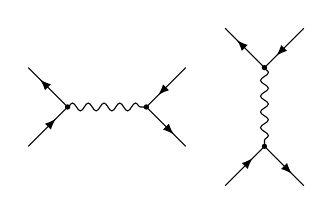
\begin{tikzpicture}[scale=0.5, baseline]
\tikzset{midarrow/.style={postaction={decorate,decoration={markings,mark=at position 0.7 with {\arrow{>}}}}}}
    \coordinate (Pi) at (-1,1);
    \coordinate (Ei) at (-1,-1);

    \coordinate (V1) at (0,0);
    \coordinate (V2) at (2,0);
    
    \coordinate (Po) at (3,1);
    \coordinate (Eo) at (3,-1);    
    
    \draw[midarrow] (V1) -- (Pi);
    \draw[midarrow] (Ei) -- (V1);
    \draw[midarrow] (Po) -- (V2);
    \draw[midarrow] (V2) -- (Eo);  

	\draw[decorate, decoration={snake, amplitude=0.5mm, segment length=2mm}] (V1) -- (V2);      
      
	\filldraw (V1) circle (1.5pt);
	\filldraw (V2) circle (1.5pt);
% % % % % % % % % % % % % % % % % % %
    \coordinate (PiS) at (5-1,2);
    \coordinate (EiS) at (5-1,-2);

    \coordinate (V1S) at (5+0,1);
    \coordinate (V2S) at (5+0,-1);
    
    \coordinate (PoS) at (5+1,2);
    \coordinate (EoS) at (5+1,-2);    
    
    \draw[midarrow] (V1S) -- (PiS);
    \draw[midarrow] (EiS) -- (V2S);
    \draw[midarrow] (PoS) -- (V1S);
    \draw[midarrow] (V2S) -- (EoS);    

	\draw[decorate, decoration={snake, amplitude=0.5mm, segment length=2mm}] (V1S) -- (V2S);      
      
	\filldraw (V1S) circle (1.5pt);
	\filldraw (V2S) circle (1.5pt);
\end{tikzpicture}
\caption{$\alpha^2$ Scattering (t-channel) and Annihilation (s-channel) - no muons}
\end{figure}

\begin{figure}[!h]
\centering
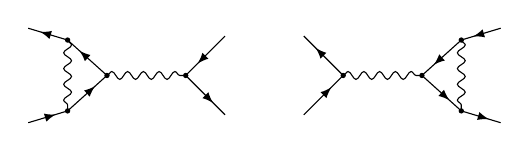
\begin{tikzpicture}[scale=0.5, baseline]
\tikzset{midarrow/.style={postaction={decorate,decoration={markings,mark=at position 0.7 with {\arrow{>}}}}}}
    \coordinate (Pi) at (-2,1.2);
    \coordinate (Ei) at (-2,-1.2);
    
    \coordinate (Pii) at (-1,0.9);
    \coordinate (Eii) at (-1,-0.9);

    \coordinate (V1) at (0,0);
    \coordinate (V2) at (2,0);
    
    \coordinate (Po) at (3,1);
    \coordinate (Eo) at (3,-1);    

    \draw[midarrow] (Pii) -- (Pi);
    \draw[midarrow] (Ei) -- (Eii);
    
    \draw[midarrow] (V1) -- (Pii);
    \draw[midarrow] (Eii) -- (V1);
    \draw[midarrow] (Po) -- (V2);
    \draw[midarrow] (V2) -- (Eo);  

	\draw[decorate, decoration={snake, amplitude=0.5mm, segment length=2mm}] (Pii) -- (Eii);
	\draw[decorate, decoration={snake, amplitude=0.5mm, segment length=2mm}] (V1) -- (V2);
      
	\filldraw (V1) circle (1.5pt);
	\filldraw (V2) circle (1.5pt);
	\filldraw (Eii) circle (1.5pt);
	\filldraw (Pii) circle (1.5pt);	
% % % % % % % % % % % % % % % % % % %
    \coordinate (Pi_2) at (6-1,1);
    \coordinate (Ei_2) at (6-1,-1);
    
    \coordinate (V1_2) at (6+0,0);
    \coordinate (V2_2) at (6+2,0);

    \coordinate (Poo_2) at (6+3,0.9);
    \coordinate (Eoo_2) at (6+3,-0.9);
    
    \coordinate (Po_2) at (6+4,1.2);
    \coordinate (Eo_2) at (6+4,-1.2);    
    
    \draw[midarrow] (V1_2) -- (Pi_2);
    \draw[midarrow] (Ei_2) -- (V1_2);
    \draw[midarrow] (Poo_2) -- (V2_2);
    \draw[midarrow] (V2_2) -- (Eoo_2);
    
    \draw[midarrow] (Po_2) -- (Poo_2);
    \draw[midarrow] (Eoo_2) -- (Eo_2);
	
	\draw[decorate, decoration={snake, amplitude=0.5mm, segment length=2mm}] (Poo_2) -- (Eoo_2);
	\draw[decorate, decoration={snake, amplitude=0.5mm, segment length=2mm}] (V1_2) -- (V2_2);
      
	\filldraw (V1_2) circle (1.5pt);
	\filldraw (V2_2) circle (1.5pt);
	\filldraw (Poo_2) circle (1.5pt);
	\filldraw (Eoo_2) circle (1.5pt);	
\end{tikzpicture}
\caption{$\alpha^4$ Scattering - no muons }
\end{figure}

\begin{figure}[!h]
\centering
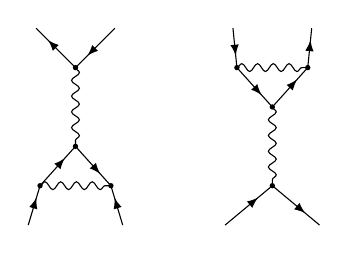
\begin{tikzpicture}[scale=0.5, baseline]
\tikzset{midarrow/.style={postaction={decorate,decoration={markings,mark=at position 0.7 with {\arrow{>}}}}}}
    \coordinate (Pi) at (-1,2);
    \coordinate (Ei) at (-1.2,-3);

    \coordinate (V1) at (0,1);
    \coordinate (V2) at (0,-1);
    
    \coordinate (Po) at (1,2);
    \coordinate (Eo) at (1.2,-3); 
    
	\coordinate (Eii) at (-0.9,-2);
    \coordinate (Eoo) at (0.9,-2);
    
    \draw[midarrow] (Po) -- (V1);
    \draw[midarrow] (V1) -- (Pi);
   
    \draw[midarrow] (Ei) -- (Eii); 
    \draw[midarrow] (Eii) -- (V2);
    \draw[midarrow] (Eo) -- (Eoo);      
    \draw[midarrow] (V2) -- (Eoo); 
   
	\draw[decorate, decoration={snake, amplitude=0.5mm, segment length=2mm}] (V1) -- (V2); 
	\draw[decorate, decoration={snake, amplitude=0.5mm, segment length=2mm}] (Eii) -- (Eoo);      
      
	\filldraw (V1) circle (1.5pt);
	\filldraw (V2) circle (1.5pt);
	\filldraw (Eii) circle (1.5pt);
	\filldraw (Eoo) circle (1.5pt);
	
% % % % % % % % % % % % % % % % % % %	
    \coordinate (Pi_2) at (5-1,3-1);
    \coordinate (Ei_2) at (5-1.2,-2-1);

    \coordinate (V1_2) at (5+0,1-1);
    \coordinate (V2_2) at (5+0,-1-1);
    
    \coordinate (Po_2) at (5+1,3-1);
    \coordinate (Eo_2) at (5+1.2,-2-1); 
    
	\coordinate (Pii_2) at (5-0.9,2-1);
    \coordinate (Poo_2) at (5+0.9,2-1);
    
    \draw[midarrow] (Poo_2) -- (Po_2);
    \draw[midarrow] (V1_2) -- (Poo_2);
   
    \draw[midarrow] (Pi_2) -- (Pii_2); 
    \draw[midarrow] (Pii_2) -- (V1_2);
    \draw[midarrow] (V2_2) -- (Eo_2); 
    \draw[midarrow] (Ei_2) -- (V2_2); 
   
	\draw[decorate, decoration={snake, amplitude=0.5mm, segment length=2mm}] (V1_2) -- (V2_2); 
	\draw[decorate, decoration={snake, amplitude=0.5mm, segment length=2mm}] (Pii_2) -- (Poo_2);      
      
	\filldraw (V1_2) circle (1.5pt);
	\filldraw (V2_2) circle (1.5pt);
	\filldraw (Pii_2) circle (1.5pt);
	\filldraw (Poo_2) circle (1.5pt);	
	
\end{tikzpicture}
\caption{$\alpha^4$ Annihilation - no muons}
\end{figure}

\begin{figure}[!h]
\centering
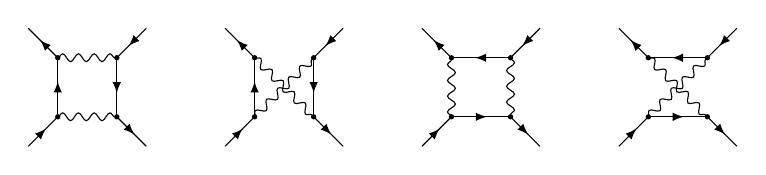
\begin{tikzpicture}[scale=0.5, baseline]
\tikzset{midarrow/.style={postaction={decorate,decoration={markings,mark=at position 0.6 with {\arrow{>}}}}}}
    \coordinate (Pi) at (-1.5,1.5);
    \coordinate (Ei) at (-1.5,-1.5);
    \coordinate (Vnw) at (-0.75,0.75);
    \coordinate (Vno) at (0.75,0.75);
    \coordinate (Vsw) at (-0.75,-0.75);
    \coordinate (Vso) at (0.75,-0.75);
    \coordinate (Po) at (1.5,1.5);
    \coordinate (Eo) at (1.5,-1.5); 
    
    \draw[midarrow] (Vnw) -- (Pi);
    \draw[midarrow] (Ei) -- (Vsw);
    \draw[midarrow] (Po) -- (Vno);
    \draw[midarrow] (Vso) -- (Eo);
   
    \draw[midarrow] (Vno) -- (Vso);
    \draw[midarrow] (Vsw) -- (Vnw);
	\draw[decorate, decoration={snake, amplitude=0.5mm, segment length=2mm}] (Vnw) -- (Vno); 
	\draw[decorate, decoration={snake, amplitude=0.5mm, segment length=2mm}] (Vsw) -- (Vso);    
      
	\filldraw (Vnw) circle (1.5pt);
	\filldraw (Vno) circle (1.5pt);
	\filldraw (Vso) circle (1.5pt);
	\filldraw (Vsw) circle (1.5pt);
% % % % % % % % % % % % % % % % % % %	
    \coordinate (Pi) at (-1.5+5,1.5);
    \coordinate (Ei) at (-1.5+5,-1.5);
    \coordinate (Vnw) at (-0.75+5,0.75);
    \coordinate (Vno) at (0.75+5,-0.75);
    \coordinate (Vsw) at (-0.75+5,-0.75);
    \coordinate (Vso) at (0.75+5,+0.75);
    \coordinate (Po) at (1.5+5,1.5);
    \coordinate (Eo) at (1.5+5,-1.5); 
    
    \draw[midarrow] (Vnw) -- (Pi);
    \draw[midarrow] (Ei) -- (Vsw);
    \draw[midarrow] (Po) -- (Vso);
    \draw[midarrow] (Vno) -- (Eo);
   
    \draw[midarrow] (Vso) -- (Vno);
    \draw[midarrow] (Vsw) -- (Vnw);
	\draw[decorate, decoration={snake, amplitude=0.5mm, segment length=2mm}] (Vnw) -- (Vno); 
	\draw[decorate, decoration={snake, amplitude=0.5mm, segment length=2mm}] (Vsw) -- (Vso);    
      
	\filldraw (Vnw) circle (1.5pt);
	\filldraw (Vno) circle (1.5pt);
	\filldraw (Vso) circle (1.5pt);
	\filldraw (Vsw) circle (1.5pt);
% % % % % % % % % % % % % % % % % % %	
    \coordinate (Pi) at (-1.5+10,1.5);
    \coordinate (Ei) at (-1.5+10,-1.5);
    \coordinate (Vnw) at (-0.75+10,0.75);
    \coordinate (Vno) at (0.75+10,0.75);
    \coordinate (Vsw) at (-0.75+10,-0.75);
    \coordinate (Vso) at (0.75+10,-0.75);
    \coordinate (Po) at (1.5+10,1.5);
    \coordinate (Eo) at (1.5+10,-1.5); 
    
    \draw[midarrow] (Vnw) -- (Pi);
    \draw[midarrow] (Ei) -- (Vsw);
    \draw[midarrow] (Po) -- (Vno);
    \draw[midarrow] (Vso) -- (Eo);
   
    \draw[midarrow] (Vno) -- (Vnw);
    \draw[midarrow] (Vsw) -- (Vso);
	\draw[decorate, decoration={snake, amplitude=0.5mm, segment length=2mm}] (Vno) -- (Vso); 
	\draw[decorate, decoration={snake, amplitude=0.5mm, segment length=2mm}] (Vsw) -- (Vnw);    
      
	\filldraw (Vnw) circle (1.5pt);
	\filldraw (Vno) circle (1.5pt);
	\filldraw (Vso) circle (1.5pt);
	\filldraw (Vsw) circle (1.5pt);
% % % % % % % % % % % % % % % % % % %	
    \coordinate (Pi) at (-1.5+15,1.5);
    \coordinate (Ei) at (-1.5+15,-1.5);
    \coordinate (Vnw) at (+0.75+15,0.75);
    \coordinate (Vno) at (-0.75+15,0.75);
    \coordinate (Vsw) at (-0.75+15,-0.75);
    \coordinate (Vso) at (0.75+15,-0.75);
    \coordinate (Po) at (1.5+15,1.5);
    \coordinate (Eo) at (1.5+15,-1.5); 
    
    \draw[midarrow] (Vno) -- (Pi);
    \draw[midarrow] (Ei) -- (Vsw);
    \draw[midarrow] (Po) -- (Vnw);
    \draw[midarrow] (Vso) -- (Eo);
   
    \draw[midarrow] (Vnw) -- (Vno);
    \draw[midarrow] (Vsw) -- (Vso);
	\draw[decorate, decoration={snake, amplitude=0.5mm, segment length=2mm}] (Vno) -- (Vso); 
	\draw[decorate, decoration={snake, amplitude=0.5mm, segment length=2mm}] (Vsw) -- (Vnw);    
      
	\filldraw (Vnw) circle (1.5pt);
	\filldraw (Vno) circle (1.5pt);
	\filldraw (Vso) circle (1.5pt);
	\filldraw (Vsw) circle (1.5pt);
\end{tikzpicture}
\caption{$\alpha^4$ Box - no muons}
\end{figure}

\begin{figure}[!h]
\centering
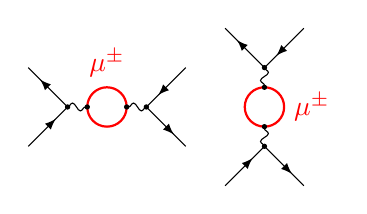
\begin{tikzpicture}[scale=0.5, baseline]
\tikzset{midarrow/.style={postaction={decorate,decoration={markings,mark=at position 0.7 with {\arrow{>}}}}}}
    \coordinate (Pi) at (-1,1);
    \coordinate (Ei) at (-1,-1);

    \coordinate (V1) at (0,0);
    \coordinate (V2) at (2,0);
    
    \coordinate (Po) at (3,1);
    \coordinate (Eo) at (3,-1);    
    
    \draw[midarrow] (V1) -- (Pi);
    \draw[midarrow] (Ei) -- (V1);
    \draw[midarrow] (Po) -- (V2);
    \draw[midarrow] (V2) -- (Eo);  

	\draw[thick, red] (1,0) circle (0.5) node[above, yshift=7pt] {$\mu^{\pm}$};

	\draw[decorate, decoration={snake, amplitude=0.5mm, segment length=2mm}] (V1) -- (0.5,0);      
	\draw[decorate, decoration={snake, amplitude=0.5mm, segment length=2mm}] (V2) -- (1.5,0);  
      
	\filldraw (V1) circle (1.5pt);
	\filldraw (V2) circle (1.5pt);
	\filldraw (0.5,0) circle (1.5pt);
	\filldraw (1.5,0) circle (1.5pt);
% % % % % % % % % % % % % % % % % % %
    \coordinate (PiS) at (5-1,2);
    \coordinate (EiS) at (5-1,-2);

    \coordinate (V1S) at (5+0,1);
    \coordinate (V2S) at (5+0,-1);
    
    \coordinate (PoS) at (5+1,2);
    \coordinate (EoS) at (5+1,-2);    
    
    \draw[midarrow] (V1S) -- (PiS);
    \draw[midarrow] (EiS) -- (V2S);
    \draw[midarrow] (PoS) -- (V1S);
    \draw[midarrow] (V2S) -- (EoS);    

	\draw[thick, red] (5+0,0) circle (0.5) node[right, xshift=7pt] {$\mu^{\pm}$};

	\draw[decorate, decoration={snake, amplitude=0.5mm, segment length=2mm}] (V2S) -- (5+0,-0.5);
	\draw[decorate, decoration={snake, amplitude=0.5mm, segment length=2mm}] (V1S) -- (5+0,+0.5);      
      
	\filldraw (V1S) circle (1.5pt);
	\filldraw (V2S) circle (1.5pt);
	\filldraw (5+0,-0.5) circle (1.5pt);
	\filldraw (5+0,+0.5) circle (1.5pt);
\end{tikzpicture}
\caption{$\alpha^4$ 1-Loop}
\end{figure}

\item

\item

\end{enumerate}



\newpage
\section{Open questions}

\begin{itemize}
\item https://www.youtube.com/playlist?list=PLtPAv05VUDZrfcGZBoJqREm7XReqP6mPV

\end{itemize}

\begin{enumerate}
\item Klein-Gordon Hamiltonian - integration by parts of $(\nabla\phi)^2$ to get $\phi\triangle\phi$ - how do we know that the $\triangle\phi$ does not contain another hidden $\phi$
\item Canonical quantization: classical field $\phi(\mathbf{x},t)$ to Heisenberg picture? 
\item guessing vs calculating Poisson brackets
\item Quantization
\begin{align}
P^\mu
&=\int d^3 x \frac{\partial\mathcal{L}}{\partial\dot{\phi}_i}(\partial^\mu\phi_i)-\eta^{\mu0}\mathcal{L}\quad\rightarrow\quad\hat{P}^\mu=\hat{P}^\mu(a,a^\dagger)\\
J^{\mu\nu}
&=\int d^3 x (T^{0\nu}x^\mu-T^{0\mu}x^\nu)\quad\rightarrow\quad\hat{J}^{\mu\nu}=\hat{J}^{\mu\nu}(a,a^\dagger)
\end{align}
what do I get for $U(\Lambda,\epsilon)=e^{-\frac{i}{2}\omega_{\mu\nu}\hat{J}^{\mu\nu}-i\epsilon_\mu\hat{P}^\mu}$
\item $\hat{P}^\mu=\hat{P}^\mu(a,a^\dagger)$ vs $\hat{P}^\mu=-i\partial_\mu$
\item 2.2.5 - 3.) Transformation law for scalar field operator $U^\dagger(\Lambda,a)\hat{\phi}(\Lambda x +a)U\dagger(\Lambda,a)=\hat{\phi}(x)$
only valid for free KG field? (because we used the free KG commutation relation)
\item Which Dirac $\gamma, S^{\mu\nu}, \Psi$ formulas are valid in general, or in special dimensions or only for special representations - is there a good overview?
\item Meaning/implications of Hermitisity of $\mathcal{L}$
\item Meaning of $\mathcal{L}=(\partial_\mu\bar{\Psi})(\partial^\mu\Psi)$
\item commutations relations between a,b and u,v?

\end{enumerate}

\chapter{Summaries}
\section{Representation Theory - Definitions}
\begin{itemize}
\item For a {\bf Lie group} $G=\{g\}$ the elements depend in a continuous and differentiable way on a set of real parameters $\theta^a$
\begin{align}
g(\theta=0)=e
\end{align}

\item A {\bf group representation} $R$ maps each group element onto a linear operator $D_R$ defined on a linear space (base space)
\begin{align}
g\rightarrow D_R(g)
\end{align}
with
\begin{itemize}
\item $D_R(e)=1$
\item $D_R(g_1)D_R(g_2)=D_R(g_1g_2)$
\end{itemize}
In case the base space is of dimension $n$ then a group element is represented by a $n\times n$ matrix and for an element of the base space $\phi=(\phi^1,..,\phi^n)$ we have
\begin{align}
\phi^i\rightarrow(D_R(g))^i_{\;j}\phi^j
\end{align}

\item {\bf Irreducible representation} (irrep) ...

\item {\bf Generators} of the group $T$
\begin{align}
D_R(\theta)&\simeq 1+i\theta^aT_R^a\\
\rightarrow T_R^a&=\left.-i\frac{\partial D_R}{\partial\theta}\right|_{\theta=0}\\
\rightarrow D_R(g(\theta))&=e^{i\theta_aT_R^a}
\end{align}
Must maintain group property
\begin{align}
D_R(g_1)&=e^{i\alpha_aT_R^a}, \qquad D_R(g_2)=e^{i\beta_bT_R^b}\\
\rightarrow D_R(g_1)D_R(g_2)&=D_R(g_1g_2)\\
\rightarrow e^{i\alpha_aT_R^a}e^{i\beta_bT_R^b}&=e^{i\delta_cT_R^c}
\end{align}

\item {\bf Lie algebra} (independent of representation) - for matrix representation the Lie bracket is just the commutator 
\begin{align}
[T^a,T^b]=if^{ab}_cT^c
\end{align}

\item {\bf Casimir operator} an operator which is NOT part of the Lie algebra but commutes with all generators

\end{itemize}


\section{Representations - fact summary}
\begin{itemize}
\item Most relevant groups (and associated Lie algebras in physics are
\begin{enumerate}
\item SO(3) - Spacial rotations in three dimensions
\item SU(2) - Angular momentum in quantum mechanics
\item SU(3) - Light quark flavour symmetry, colors in QCD
\item SL(2,$\mathbb{C}$) - Lorentz group
\item SO$(1,3)^+$ - (vector rep. of Lorentz group)
\item ISO$(1,3)\sim\mathbb{R}^{1,3}\times$O(1,3) - Poincare transformations
\item Sp(2$n,\mathbb{R}$) - Hamiltonian systems
\end{enumerate}
\item {\bf SU(2)}: To get a systematic overview (of representations  which are relevant in physics) it is best to start with group SU(2) - because most of the following can be derived from here
\begin{itemize}
\item the $j=\sfrac{1}{2}$ (2-dimensional defining) representation of the group follows from 2d geometry
\begin{align}
\left(\begin{matrix}
\alpha & -\bar{\beta}\\
\beta & \bar{\alpha}\\
\end{matrix}\right)\qquad\text{with }|\alpha|^2+|\beta|^2=1
\end{align}
\item from this we derive the 2d representation of generators (of the Lie algebra $\mathfrak{su}(2)$) which is given by $L_k=\sigma_k/2$ (Pauli matrices)
\item Lie algebra can then be calculated for this representation (which holds for any representation) 
\begin{align}
[L_i,L_j]=i\epsilon_{ijk}L_k
\end{align}
\item one Casimir operator: $L^2=L_1^2+L_2^2+L_3^2$ with $[L^2,L_k]=0$
\item exactly one irrep for each $j=0,\sfrac{1}{2},1,\sfrac{3}{2},2,...$ (dimension $n=2j+1$) - construction:
\begin{enumerate}
\item start with $n=2j+1$ dimensional orthogonal euclidean basis $|jm_j\rangle$ ($-j\le m_j\le j$)
\item action $L_\pm=L_x\pm iL_y$ and $L^2$ on them (using generic properties of the operators) 
\item calculate all matrix elements $\langle jm'|L_\pm|jm\rangle$ and $\langle jm'|L^2|jm\rangle$ - obtaining the representation of $L_\pm$ and $L^2$
\item then calculate matrix representation of $L_k$
\end{enumerate}
\item for spin-$j$ irreps of the Lie algebra the $2j+1$-dimensional representation space is spanned by $\{|j,-j\rangle, ...,|j,+j\rangle\}$
\begin{itemize}
\item {\bf Tensor representations of the Lie algebra} $\mathfrak{su}(2)$ for $j=0,1,2,3,...$ (with odd dimensions $1,3,4,\cdots$) the associated group-irreps are $2\pi$ periodic
\item {\bf Spinor representations of the Lie algebra} $\mathfrak{su}(2)$ for $j=\sfrac{1}{2},\sfrac{3}{2},\sfrac{5}{2},...$ (with even dimensions $2,4,6,\cdots$) we have
\begin{align}
D_R(g_{\theta=2\pi})=e^{iL_k\cdot 2\pi}=-1
\end{align}
meaning the associated group-irreps are not $2\pi$ but $4\pi$ periodic
\end{itemize}
\item Clebsch-Gordon decomposition of tensor product of representations
\begin{align}
&D_{j_1}\otimes D_{j_2}=D_{|j_1-j_2|}\oplus...\oplus D_{j_1+j_2}\\
&\rightarrow D_{\sfrac{1}{2}}\otimes D_{\sfrac{1}{2}}=D_0\oplus D_1\qquad(\mathbf{2\otimes2=1\oplus3})\\
&\rightarrow D_{\sfrac{1}{2}}\otimes D_{\sfrac{1}{2}}\otimes D_{\sfrac{1}{2}}=(D_0\otimes D_{\sfrac{1}{2}})\oplus (D_1\otimes D_{\sfrac{1}{2}})=D_{\sfrac{1}{2}}\otimes D_{\sfrac{1}{2}} \otimes D_{\sfrac{3}{2}}\\
&\rightarrow D_{\sfrac{3}{2}}\otimes D_{\sfrac{3}{2}}=D_0\oplus D_1\oplus D_2\oplus D_3\qquad(\mathbf{4\otimes4=1\oplus3\oplus5\oplus7})
\end{align}

\end{itemize}

\item {\bf SO(3)}
\begin{itemize}
\item the 3-dimensional (defining) representation of the group follows from 3d geometry
\item three generators of the $\mathfrak{so}(3)$ follow from  derivatives of the three basis rotation matrices
\item same Lie algebra as SU(2)
\begin{align}
[L_i,L_j]=i\epsilon_{ijk}L_k
\end{align}
(so both groups look similar near the $1$-element)
\item one Casimir Operator: $L^2=L_x^2+L_y^2+L_z^2$
\item SU(2) is the universal covering group of SO(3)
\item Irreps
\begin{itemize}
\item Lie algebra $\mathfrak{so}(3)$ has same tensor and spinor irreps as $\mathfrak{su}(2)$
\item Lie group SO(3) shares only tensor irreps as of SU(2) - as spinor irreps are $4\pi$ periodic
\end{itemize}
\end{itemize}

\item {\bf SO(1,3) or  SL(2,$\mathbb{C}$) - Lorentz group}
\begin{itemize}
\item 4-dimensional defining representation ($x'^\mu=\Lambda^\mu_{\;\nu}x^\nu$) follows from $g_{\mu\nu}=\Lambda^\rho_{\;\mu}\Lambda^\sigma_{\;\nu}g_{\rho\sigma}$ - rotations four dimensional $1+3$ coordinates (signature $+,-,-,-$) therefore SO(1,3)
\item side note: relation with SL(2,$\mathbb{C}$)
\begin{align}
x^\mu\rightarrow X\equiv\sigma_\mu x^\mu
&=\left(
\begin{matrix}
x^0+x^3   & -x^1-ix^2\\
-x^1+ix^2 & x^0-x^3\\
\end{matrix}
\right)\\
&\rightarrow\det X=(x^0)^2-\mathbf{x}^2
\end{align}
then a Lorentz transformation can be represented by $A(\Lambda)$ with
\begin{align}
X\overset{\Lambda}{\rightarrow}X'&=A(\Lambda)XA^\dagger(\Lambda)\\
&\rightarrow \det X'=\det A\det X\det A^\dagger
\end{align} 
so $A$ is really a Lorentz transformation if $\det A\det A^\dagger=|\det A|^2=1$ meaning 
$A(\Lambda)\in\,$SL(2,$\mathbb{C}$) - (ignoring the overall phase of $A$)
\item \textcolor{red}{open question - can the matrix $X$ be expressed as a complex 2-vector  or spinor}
\item infinitesimal Lorentz transformation $x^\mu\simeq[\delta^\mu_\nu-\frac{i}{2}(\omega_{\rho\sigma}J^{\rho\sigma})^\mu_{\;\nu}]x^\nu$ can be found by derivative with respect to the six parameters $\omega_{\mu\nu}=-\omega_{\nu\mu}$ and the 6 generators can be written in the 4-dimensional representation as
\begin{align}
(J^{\mu\nu})^\rho_{\;\sigma}
&=i(g^{\mu\rho}\delta^\nu_\sigma-g^{\nu\rho}\delta^\mu_\sigma)
\end{align}
\item from this we can obtain the Lie algebra by just calculating the commutators
\item so there are three forms
\begin{enumerate}
\item we obtain form this directly
\begin{align}
[J^{\mu\nu},J^{\rho\sigma}]
&=if^{\mu\nu\rho\sigma}_{\qquad\alpha\beta}J^{\alpha\beta}\\
&=-i(g^{\mu\rho}J^{\nu\sigma}-g^{\mu\sigma}J^{\nu\rho}+g^{\nu\rho}J^{\mu\sigma}-g^{\nu\sigma}J^{\mu\rho})
\end{align}
\item rearranging 3 boosts $K_i=J^{0i}$ and 3 rotations $J_i=\frac{1}{2}\epsilon_{ijk}J^{jk}$ into two vectors $\mathbf{J,K}$ with algebra
\begin{align}
[J_i,J_j]&=i\epsilon_{ijk}J_k\\
[K_i,K_j]&=-i\epsilon_{ijk}J_k\\
[J_i,K_j]&=i\epsilon_{ijk}K_k\\
&\rightarrow\Lambda=\exp\left[\pmb{\theta}\cdot\mathbf{J}-\pmb{\eta}\cdot\mathbf{K}\right]
\end{align}
\item rearranging again $\mathbf{J}^\pm=\frac{\mathbf{J}\pm i\mathbf{K}}{2}$ gives
\begin{align}
[J^{+,i},J^{+,j}]&=i\epsilon^{ijk}J^{+,k}\\
[J^{-,i},J^{-,j}]&=i\epsilon^{ijk}J^{-,k}\\
[J^{+,i},J^{-,j}]&=0
\end{align}
two copies of $\mathfrak{su}(2)$ which commute between themselves
\end{enumerate}
\item $\mathfrak{sl}(2,\mathbb{C})=\mathfrak{su}(2)\otimes\mathfrak{su}(2)$ but 
\begin{itemize}
\item SU(2)$\otimes$SU(2) is the universal covering group of SO(4)
\item SO(3,1) is the universal covering group of SL(2,$\mathbb{C}$)
\end{itemize}
\item two Casimir operators
\begin{itemize}
\item $C_1=\frac{1}{2}J_{\mu\nu}J^{\mu\nu}=\vec{J}^2-\vec{K}^2=\vec{J^+}^2+\vec{J^-}^2$
\item $C_2=\frac{1}{2}\epsilon_{\mu\nu\rho\sigma}J^{\mu\nu}J^{\rho\sigma}=\vec{J}\cdot\vec{K}=i(\vec{J^+}^2-\vec{J^-}^2)$
\end{itemize} 
\item Using the $\mathfrak{su}(2)$ irreps - the Lorentz algebra irreps can be labeled 
\begin{align}
(j_-,j_+)=(j_-,0)\otimes(0,j_+)
\end{align}
and because $\mathbf{J}=\mathbf{J}^+ + \mathbf{J}^-$ we have states a spins between $|j_--j_+|,...,j_-+j_+$
\begin{itemize}
\item {\bf Scalar representation} $(0,0)$ the spin $0$ irrep - acting on $(2\cdot0+1)(2\cdot0+1)=1$ dimensional objects - scalars
\begin{align}
J_S^{\mu\nu}=0
&\quad\rightarrow\quad\Lambda^\mu_{\;\nu}=1\\
&\quad\rightarrow\quad\phi\rightarrow1\cdot\phi
\end{align}

\item {\bf Weyl spinor representation} fundamental spinorial representations - there are two distinct spin $\sfrac{1}{2}$ irreps - acting on $(2\cdot0+1)(2\cdot1+1)=2$ dimensional objects - Weyl spinors
\begin{itemize}
\item {\bf Left-handed Weyl spinor} ($\sfrac{1}{2},0$) - so $\mathbf{J}^-=\pmb{\sigma}/2$ and $\mathbf{J}^+=0$ then $\mathbf{J}=\pmb{\sigma}/2$ and $\mathbf{K}=+i\pmb{\sigma}/2$
\begin{align}
J_L^{\mu\nu}=S^{\mu\nu},\quad 
S^{ij}=\frac{1}{2}\epsilon^{ijk}\sigma_k, 
S^{0i}=-\frac{i}{2}\sigma^i
\quad\rightarrow\quad e^{-\frac{i}{2}\omega_{\mu\nu}S^{\mu\nu}}=\Lambda_L\\
\psi_L\rightarrow\Lambda_L\psi_L=\exp\left[(-i\pmb{\theta}-\pmb{\eta})\cdot\frac{\pmb{\sigma}}{2}\right]\psi_L
\end{align}
\item {\bf Right-handed Weyl spinor} ($0,\sfrac{1}{2}$) - so $\mathbf{J}^-=0$ and $\mathbf{J}^+=\pmb{\sigma}/2$ then $\mathbf{J}=\pmb{\sigma}/2$ and $\mathbf{K}=-i\pmb{\sigma}/2$
\begin{align}
J_R^{\mu\nu}=S^{\mu\nu},\quad 
S^{ij}=\frac{1}{2}\epsilon^{ijk}\sigma_k, 
S^{0i}=+\frac{i}{2}\sigma^i
\quad\rightarrow\quad e^{-\frac{i}{2}\omega_{\mu\nu}S^{\mu\nu}}=\Lambda_R\\
\psi_R\rightarrow\Lambda_R\psi_R=\exp\left[(-i\pmb{\theta}+\pmb{\eta})\cdot\frac{\pmb{\sigma}}{2}\right]\psi_R
\end{align}
\end{itemize}
we also see that $\sigma_2\psi_L^*$ transforms like a right handed spinor and define the charge conjugate of a Weyl spinor as  $\psi_L^c=i\sigma_2\psi_L^*$ and $\psi_R^c=-i\sigma_2\psi_R^*$
\item {\bf 4-vector representation} (\sfrac{1}{2},\sfrac{1}{2}) spin 0,1 irrep acting on $(2\cdot\sfrac{1}{2}+1)(2\cdot\sfrac{1}{2}+1)=4$ dimensional objects - 4-vectors
\begin{align}
(J_V^{\mu\nu})^\rho_{\;\sigma}
&=i(g^{\mu\rho}\delta^\nu_\sigma-g^{\nu\rho}\delta^\mu_\sigma)\quad\rightarrow\quad (e^{-\frac{i}{2}\omega_{\mu\nu}J^{\mu\nu}})^\rho_{\;\sigma}=\Lambda^\rho_{\;\sigma}
\end{align}
with $\sigma^\mu=(1,\sigma^k)$ and $\bar{\sigma}^\mu=(1,-\sigma^k)$ we see that $\xi_R^\dagger\sigma^\mu\psi_R$ and $\xi_L^\dagger\bar{\sigma}^\mu\psi_L$ are (transform like) 4-vectors
\item {\bf Dirac spinor representation} $(\sfrac{1}{2},0)\oplus(0,\sfrac{1}{2})$ reducible representation action on $2+2=4$ dimensional objects - Dirac spinors
\begin{align}
S^{ij}=\frac{1}{2}\epsilon^{ijk}\left(\begin{matrix}
\sigma^k & 0\\
0 & \sigma^k
\end{matrix}
\right),\qquad
S^{0i}=-\frac{1}{2}\left(\begin{matrix}
\sigma^i & 0\\
0 & -\sigma^i
\end{matrix}
\right)\\
J_D^{\mu\nu}=S^{\mu\nu}=\frac{i}{4}[\gamma^\mu,\gamma^\nu]\quad\rightarrow\quad e^{-\frac{i}{2}\omega_{\mu\nu}S^{\mu\nu}}=\Lambda_D\\
\left(\begin{matrix}
\psi_L \\ \psi_R
\end{matrix}
\right)\rightarrow\Lambda_D\left(\begin{matrix}
\psi_L \\ \psi_R
\end{matrix}
\right)
\end{align}
\item {\bf Infinite-dimensional Orbital representation} the $L^{ij}$ are the classical generators of angular momentum 
\begin{align}
L^{\mu\nu}=x^\mu\partial_\nu-x^\nu\partial_\mu
\end{align}
\end{itemize}
\item Field - with $\left(e^{-\frac{i}{2}\omega_{\mu\nu}J_V^{\mu\nu}}\right)^\rho_{\;\sigma}x^\sigma
\simeq\left(1-\frac{i}{2}\omega_{\mu\nu}i(g^{\mu\rho}\delta^\nu_\sigma-g^{\nu\rho}\delta^\mu_\sigma)\right)x^\sigma=x^\sigma+\omega^\sigma_{\;\mu} x^\mu$
\begin{align}
\Phi_a\rightarrow M_{ab}(\Lambda)\Phi_b
\qquad\Rightarrow\qquad
\Phi_a(x)\rightarrow \Phi'_a(x)&=M_{ab}(\Lambda)\Phi_b(\Lambda^{-1}x)\\
L^{\mu\nu}=i(x^\mu\partial^\nu-x^\nu\partial^\mu)
\qquad\Rightarrow\qquad
e^{-\frac{i}{2}\omega_{\mu\nu}L^{\mu\nu}}\Phi(x)
&=\left(1-\frac{i}{2}\omega_{\mu\nu}L^{\mu\nu}\right)\Phi(x)\\
&=\Phi(x)+(\partial^\nu\Phi)\cdot \omega_{\mu\nu}x^\mu\\
&=\Phi(x+\omega_\mu^{\;\nu}x^\mu)\\
&=\Phi(\Lambda^{-1}x)
\end{align}
then with $L^{\mu\nu}+J^{\mu\nu}$
\begin{align}
\Phi_a(x)\rightarrow \Phi'_a(x)
&=\left(e^{-\frac{i}{2}\omega_{\mu\nu}J^{\mu\nu}}\right)_{ab}e^{-\frac{i}{2}\omega_{\mu\nu}L^{\mu\nu}}\Phi_b(x)\\
&=\left(e^{-\frac{i}{2}\omega_{\mu\nu}J^{\mu\nu}}\right)_{ab}\Phi_b(\Lambda^{-1}x)
\end{align}

\end{itemize}

\item {\bf Poincare group}
\begin{itemize}
\item Lie algebra (\textcolor{red}{Lorentz}, \textcolor{blue}{just translation}, \textcolor{purple}{Lorentz/translations})
\begin{align}
\textcolor{red}{[M^{\mu\nu},M^{\rho\sigma}]=-i(g^{\mu\rho}M^{\nu\sigma}-g^{\mu\sigma}M^{\nu\rho}+g^{\nu\rho}M^{\mu\sigma}-g^{\nu\sigma}M^{\mu\rho})}\\
\textcolor{blue}{[P^\mu,P^\nu]=0}\\
\textcolor{purple}{[P^\mu,M^{\rho\sigma}]=i(g^{\mu\rho}P^\sigma-g^{\mu\sigma}P^\rho)}
\end{align}
\item One Casimir operator: $L^2=L_1^2+L_2^2+L_3^2$ with $[L^2,L_k]=0$
\begin{enumerate}
\item $\mathcal{M}^2=P_\mu P^\mu$ squared mass
\item $\mathcal{W}^2=W_\mu W^\mu$ with Pauli-Lubaniski vector $W_\mu=\frac{1}{2}\epsilon_{\mu\nu\rho\sigma} J^{\nu\rho}P^\sigma$
\end{enumerate}
\end{itemize}

\end{itemize}


\section{Spacetime Transformations}
\subsection{Lorentz Transformations}
Exam question: {\it Whats the defining property of a Lorentz transformation?}
\begin{itemize}
\item Answer: It is a transformation on the spacetime coordinates $x'^\mu=\Lambda^\mu_{\;\nu}x^\nu$ which leaves the line element $ds^2=\eta_{\mu\nu}dx^\mu dx^\nu$ invariant.
\item Physical substance: Speed of light $c$ is the same in each inertial system.
\item Expressed mathematically:
$\eta_{\mu\nu}=\Lambda^\alpha_{\,\mu}\Lambda^\beta_{\,\nu}\eta_{\alpha\beta}$
\end{itemize}
The common Lorentz transformation law of a 4-vector
\begin{align}
V'^\mu=\Lambda^\mu_{\;\nu}V^\nu
\end{align}
provides us naturally (each transformation is associated with a $4\times4$ matrix - obeying the definition of a representation) with a \textcolor{blue}{4-dimensional representation of the Lorentz group} meaning
\begin{align}
D_\text{4-dim}(\Lambda)=\Lambda^\mu_{\;\sigma}.
\end{align}
Now consider an infinitesimal Lorentz transformation 
\begin{align}
\Lambda^\mu_{\,\nu}
&\simeq\delta^\mu_{\,\nu}+\omega^\mu_{\,\nu}\qquad(\omega_{\mu\nu}=-\omega_{\nu\mu})\\
&\rightarrow x'^\mu
=\Lambda^\mu_{\,\nu}x^\nu\simeq x^\mu+\omega^\mu_{\,\nu}x^\nu
\end{align}
with
\begin{align}
\omega^\mu_{\,\nu}=\left(
\begin{array}{cccc}
0      &  \eta_1 &  \eta_2 &  \eta_3\\
\eta_1 &  0   & -\theta_3 &  \theta_2\\
\eta_2 &  \theta_3 &  0   & -\theta_1\\
\eta_3 & -\theta_2 &  \theta_1 &  0
\end{array}
\right)
\end{align}
The antisymmetry of $\omega$ implies that there are only 6 independent parameters (3 infinitesimal boosts $\eta_i$ and 3 infinitesimal rotations, i.e. $\theta_1$ rotation in the $2-3$ plane). {\it It would be actually more consistent to write $d\eta$ and $d\theta$.}

Now we can do a technical step - splitting the $\omega$
\begin{align}
\omega^\rho_{\,\sigma}\rightarrow -\frac{i}{2}(\omega_{\mu\nu} J^{\mu\nu})^\rho_{\,\sigma}\simeq
\eta_1\left(\begin{matrix}
0&i&0&0\\
i&0&0&0\\
0&0&0&0\\
0&0&0&0
\end{matrix}
\right)+\eta_2....+\theta_{23}....
\end{align}
which means we can write an infinitesimal trafo as
\begin{align}
D(d\Lambda)^\rho_{\;\sigma}&\simeq \delta^\rho_\sigma-\frac{i}{2}\omega_{\mu\nu}\cdot(J_R^{\mu\nu})^\rho_{\;\sigma}\\
&=\delta^\rho_\sigma-i(\omega_{01}J_R^{01}+\omega_{02}J_R^{02}+\omega_{03}J_R^{03}+\omega_{12}J_R^{12}+\omega_{23}J_R^{23}+\omega_{13}J_R^{13})\\
&=\delta^\rho_\sigma-i(\eta_1 J_R^{01}+\eta_2 J_R^{02}+\eta_3 J_R^{03}+\theta_3 J_R^{12}+\theta_1J_R^{23}+\theta_2 J_R^{13})
\end{align}
where (in our special example) the $J^{\mu\nu}_R$ are $4\times4$ matrices which can we read off from the shape of $\omega^\mu_\nu$.
In our example of the 4-dimensional (defining) representation we can write the so called generators $J^{\mu\nu}$ explicitly
\begin{align}J^{01}_\text{4-dim}=\left(
\begin{array}{cccc}
 0  &  \textcolor{red}{+i} &  0 &  0\\
\textcolor{red}{+i}  &  0 &  0 &  0\\
 0  &  0 &  0 &  0\\
 0  &  0 &  0 &  0
\end{array}
\right),\qquad
J^{23}_\text{4-dim}=\left(
\begin{array}{cccc}
0  &  0 &  0 &  0\\
0  &  0 &  0 &  0\\
0  &  0 &  0 &  \textcolor{red}{+i}\\
0  &  0 & \textcolor{red}{-i} &  0
\end{array}
\right)
\end{align}
or shorter as $(J_\text{4-dim}^{\mu\nu})^\rho_{\;\sigma}=i(\eta^{\mu\rho}\delta^\nu_\sigma-\eta^{\nu\rho}\delta^\mu_\sigma)$ - which is \textcolor{blue}{the 4-dimensional representation of the generators}.
The associated representations of the (infinitesimal) transformations are given by
\begin{align}
D_\text{4-dim}(d\Lambda^{01})=\left(
\begin{array}{cccc}
 1  &  \eta_1 &  0 &  0\\
\eta_1  &  1 &  0 &  0\\
 0  &  0 &  1 &  0\\
 0  &  0 &  0 &  1
\end{array}
\right),\qquad
D_\text{4-dim}(d\Lambda^{23})=\left(
\begin{array}{cccc}
1  &  0 &  0 &  0\\
0  &  1 &  0 &  0\\
0  &  0 &  1 &  \theta_1\\
0  &  0 & -\theta_1 &  1.
\end{array}
\right).
\end{align}
To be consistent - they should (when promoted to finite transformations) be identical with the defining 4-dimensional representation of the Lorentz group mentioned above.
\begin{align}
e^{\delta^\rho_\sigma-\frac{i}{2}\omega_{\mu\nu}(J_\text{4-dim}^{\mu\nu})^\rho_{\;\sigma}}\equiv D_\text{4-dim}(\Lambda)=\Lambda^\rho_{\;\sigma}
\end{align}

We can verify that the $(J_\text{4-dim}^{\mu\nu})^\rho_{\;\sigma}$ are indeed correct by using them to perform infinitesimal Lorentz transformations (spacetime 4-vectors) and comparing with expected result
\begin{align}
x'^\rho
&=D_\text{4-dim}(\Lambda)^\rho_{\,\sigma}x^\sigma\\
&=[\delta^\rho_\sigma-i\omega i(\eta^{\mu\rho}\delta^\nu_\sigma-\eta^{\nu\rho}\delta^\mu_\sigma)]x^\sigma\\
&=x^\rho+\omega(\eta^{\mu\rho}x^\nu-\eta^{\nu\rho}x^\mu)
\end{align}
so
\begin{align}
D_\text{4-dim}(\Lambda^{01})\qquad\rightarrow\delta x^\mu=(+\eta_1 x,+\eta_1 t,0,0)\\
D_\text{4-dim}(\Lambda^{23})\qquad\rightarrow\delta x^\mu=(0,-\theta_1 y,+\theta_1 x,0)
\end{align}
which is consistent with the expected result for an infinitesimal boost and a rotation.

Keep in mind that depending of the representation the $J_R^{\mu\nu}$ can have arbitrary dimension $n$. 

Alternatively we can write
\begin{align}
K^i\equiv J^{i0},
\qquad 
J^i\equiv\frac{1}{2}\epsilon^{ijk}J^{jk}\quad(J^{jk}=\epsilon^{jki}J^i)\qquad\rightarrow\qquad&\Lambda^\rho_{\;\sigma}
=e^{i\mathbf{\eta}\cdot\mathbf{K}-i\mathbf{\theta}\cdot\mathbf{J}}\\
\rightarrow\qquad
&[\hat{J}_i,\hat{J}_j]=i\epsilon_{ijk}\hat{J}_k\\
&[\hat{J}_i,\hat{K}_j]=i\epsilon_{ijk}\hat{K}_k\\
&[\hat{K}_i,\hat{K}_j]=-i\epsilon_{ijk}\hat{J}_k
\end{align}
with the Casimir operators $C_1=\frac{1}{2}J^{\mu\nu}J_{\mu\nu}=\mathbf{J}^2-\mathbf{K}^2$ and $C_1=\frac{1}{2}\tilde{J}^{\mu\nu}J_{\mu\nu}=\mathbf{J}\cdot\mathbf{K}$
where the dual $\tilde{J}_{\mu\nu}=\epsilon_{\mu\nu\alpha\beta}J^{\alpha\beta}$



or even
\begin{align}
\mathbf{A}=\frac{1}{2}(\mathbf{K}-i\mathbf{J})
\qquad
\mathbf{B}=\frac{1}{2}(\mathbf{K}+i\mathbf{J})
\qquad\rightarrow\qquad
&\Lambda^\rho_{\;\sigma}
=e^{i\mathbf{\eta}\cdot(\mathbf{A+B})-\mathbf{\theta}\cdot(\mathbf{B}-\mathbf{A})}\\
&\;\;\;\;\;
=e^{(i\mathbf{\eta}+\theta)\cdot\mathbf{A}+(i\eta-\mathbf{\theta})\cdot\mathbf{B}}\\
\qquad\rightarrow\qquad
&[\hat{A}_i,\hat{A}_j]=i\epsilon_{ijk}\hat{A}_k\\
&[\hat{B}_i,\hat{B}_j]=i\epsilon_{ijk}\hat{B}_k\\
&[\hat{A}_i,\hat{B}_j]=0
\end{align}
Here we obtained to two copies of an $SU(2)$ algebra, with Casimir operators $\mathbf{A}^2=\frac{1}{4}(\mathbf{K}^2-\mathbf{J}^2)-2i\mathbf{K\cdot J}$ and $\mathbf{B}^2=\frac{1}{4}(\mathbf{K}^2-\mathbf{J}^2)+2i\mathbf{K\cdot J}$

\subsection{Poincare transformations I}
For a poincare trafo we can translate first and then rotate
\begin{align}
x'^\mu
&=x^\mu+a^\mu\\
x''^\mu
&=(\delta^\mu_\nu+\omega^\mu_\nu)(x^\mu+a^\mu)\\
&=x^\mu+(\omega^\mu_\nu x^\nu)+(a^\mu+\omega^\mu_\nu a^\nu)
\end{align} 
or first rotate and then translate
\begin{align}
x'^\mu
&=x^\mu+\omega^\mu_\nu x^\nu\\
x''^\mu
&=x^\mu+(\omega^\mu_\nu x^\nu)+(a^\mu)
\end{align}
The second is commonly considered to be a Poincare trafo.


\subsection{Poincare transformations II}
\subsubsection{Coordinates}
With the defining representation $\Lambda^\mu_{\;\nu}=\left(e^{-\frac{i}{2}\omega_{\alpha\beta}\mathcal{J}^{\alpha\beta}}\right)^\mu_{\;\nu}\simeq\delta^\mu_{\;\nu}-\frac{i}{2}(\omega_{\alpha\beta}\mathcal{J}^{\alpha\beta})^\mu_{\;\nu}=\delta^\mu_{\;\nu}+\frac{1}{2}(\omega^\mu_{\,\beta}\delta^\beta_\nu-\omega_\alpha^{\;\mu}\delta^\alpha_\nu)=\delta^\mu_{\;\nu}+\omega^\mu_{\,\nu}$ using the representation of the Lie algebra $(\mathcal{J}^{\alpha\beta})^\mu_{\;\nu}=i(g^{\alpha\mu}\delta^\beta_\nu-\delta^\alpha_\nu g^{\beta\mu})$
\begin{align}
x'&=\Lambda x+a\simeq x+\omega x+\epsilon\\
\textcolor{ForestGreen}{\delta x^\alpha}&\equiv x'^\alpha-x^\alpha\\
&=\textcolor{ForestGreen}{\omega^\alpha_{\;\beta}x^\beta+\epsilon^\alpha}
\end{align}

\subsubsection{In general - multi-component fields transform like}
General assumption: theory is Poincare invariant - so a field (aka particle) must transform under a representation of the Poincare group
\begin{align}
\phi'_i(x')=R_i^{\;j}(\Lambda)\phi_j(x)
\end{align}


\subsubsection{Scalar field - (spin 0 representation)}
Most trivial case with $R(\Lambda)=1$
\begin{align}
\phi'(\Lambda x+a)=\phi(x)\qquad&\rightarrow\qquad \phi'(x)=\phi(\Lambda^{-1}x)\\
\qquad&\rightarrow\qquad \phi'(x)\simeq\phi(x-\omega x-\epsilon)
\end{align}
then
\begin{align}
\delta\phi(x)
&\equiv\phi'(x)-\phi(x)\\
&\simeq\phi(x-[\textcolor{ForestGreen}{\omega x+\epsilon}])-\phi(x)\\
&=\partial_\mu\phi(x)\cdot(-\textcolor{ForestGreen}{\delta x})\\
&=-\omega^{\mu\nu}x_\nu\partial_\mu\phi(x)-\epsilon^\mu\partial_\mu\phi(x)\\
&=-\frac{1}{2}\omega_{\mu\nu}(x^\nu\partial^\mu-x^\mu\partial^\nu)\phi(x)-\epsilon^\mu\partial_\mu\phi(x)\\
&=-\frac{i}{2}\omega_{\mu\nu}L^{\mu\nu}\phi(x)-\epsilon^\mu\partial_\mu\phi(x)
\end{align}
with $L^{\mu\nu}=-i(x^\nu\partial^\mu-x^\mu\partial^\nu)$

\subsubsection{Vector field - (spin 1 representation)}
The second most trivial case $R(\Lambda)=\Lambda^\mu_{\;\nu}=\left(e^{-\frac{i}{2}\omega_{\alpha\beta}\mathcal{J}^{\alpha\beta}}\right)^\mu_{\;\nu}\simeq\delta^\mu_{\;\nu}-\frac{i}{2}(\omega_{\alpha\beta}\mathcal{J}^{\alpha\beta})^\mu_{\;\nu}=\delta^\mu_{\;\nu}+\frac{1}{2}(\omega^\mu_{\,\beta}\delta^\beta_\nu-\omega_\alpha^{\;\mu}\delta^\alpha_\nu)=\delta^\mu_{\;\nu}+\omega^\mu_{\,\nu}$ with the representation of the Lie algebra $(\mathcal{J}^{\alpha\beta})^\mu_{\;\nu}=i(g^{\alpha\mu}\delta^\beta_\nu-\delta^\alpha_\nu g^{\beta\mu})$
\begin{align}
A'^\mu(\Lambda x+a)=\textcolor{red}{\Lambda^\mu_{\;\nu}}A^\nu(x)\qquad&\rightarrow\qquad A'^\mu(x)=\Lambda^\mu_{\;\nu}A_\nu(\Lambda^{-1}x)\\
\qquad&\rightarrow\qquad A'^\mu(x)\simeq (\delta^\mu_{\;\nu}\textcolor{red}{-\frac{i}{2}(\omega_{\alpha\beta}\mathcal{J}^{\alpha\beta})^\mu_{\;\nu}})A^\nu(x-\omega x-\epsilon)
\end{align}
then
\begin{align}
\delta A^\mu(x)
&\equiv A'^\mu(x)-A^\mu(x)\\
&=\delta^\mu_{\;\nu}A^\nu(x-\omega x-\epsilon)\textcolor{red}{-\frac{i}{2}(\omega_{\alpha\beta}\mathcal{J}^{\alpha\beta})^\mu_{\;\nu}}A^\nu(x-\omega x-\epsilon)-A^\mu(x)\\
&=\left(A^\mu(x)+\partial_\alpha A^\mu(x)[-\omega^{\alpha\beta}x_\beta-\epsilon^\alpha]+...\right)\textcolor{red}{-\frac{i}{2}(\omega_{\alpha\beta}\mathcal{J}^{\alpha\beta})^\mu_{\;\nu}}A^\nu(x)+\mathcal{O}(\omega^2)-A^\mu(x)\\
&=-\omega^{\alpha\beta}x_\beta\partial_\alpha A^\mu(x)-\epsilon^\alpha\partial_\alpha A^\mu(x)\textcolor{red}{-\frac{i}{2}(\omega_{\alpha\beta}\mathcal{J}^{\alpha\beta})^\mu_{\;\nu}}A^\nu(x)\\
&=-\frac{i}{2}\omega_{\alpha\beta}L^{\alpha\beta} A^\mu-\epsilon^\alpha\partial_\alpha A^\mu\textcolor{red}{-\frac{i}{2}(\omega_{\alpha\beta}\mathcal{J}^{\alpha\beta})^\mu_{\;\nu}}A^\nu(x)\\
&=-\frac{i}{2}\omega_{\alpha\beta}\left(L^{\alpha\beta}A^\mu+(\textcolor{red}{\mathcal{J}^{\alpha\beta}}\right)^\mu_{\;\nu} A^\nu)-\epsilon^\alpha\partial_\alpha A^\mu
\end{align}

\subsubsection{Spinor field - (spin $\sfrac{1}{2}$ representation)}
Now the group rep. is $M_{\alpha\beta}=e^{-\frac{1}{2}\omega_{\mu\nu}S^{\mu\nu}}$ with $S^{\mu\nu}=\frac{i}{4}[\gamma_\mu,\gamma_\nu]$ (so $S^{\mu\nu}$ is a representation of the Lorentz algebra - which is automatically the case if $\{\gamma^\mu,\gamma^\nu\}=2g^{\mu\nu}\times1_{n\times n}$)
\begin{align}
\Psi'_\alpha(\Lambda x+a)=M_{\alpha\beta}(\Lambda)\Psi_\beta(x)\qquad&\rightarrow\qquad\Psi'_\alpha(x)\simeq\left(\delta_{\alpha\beta}-\textcolor{blue}{\frac{i}{2}(\omega_{\mu\nu}S^{\mu\nu})_{\alpha\beta}}\right)\Psi_\beta(x-\omega x-\epsilon)
\end{align}
then
\begin{align}
\delta\Psi_\alpha(x)
&\equiv\Psi_\alpha'(x)-\Psi_\alpha(x)\\
&\simeq\partial_\mu\Psi_\alpha(-\textcolor{ForestGreen}{\delta x})-\textcolor{blue}{\frac{i}{2}(\omega_{\mu\nu}S^{\mu\nu})_{\alpha\beta}}\Psi_\beta(x)\\
&\simeq(-\omega^{\mu\nu}x_\nu-\epsilon^\mu)\partial_\mu\Psi_\alpha-\textcolor{blue}{\frac{i}{2}\omega_{\mu\nu}(S^{\mu\nu})_{\alpha\beta}}\Psi_\beta(x)\\
&=-\frac{i}{2}\omega_{\rho\sigma}\left(L^{\rho\sigma}\Psi_\alpha(x)+\textcolor{blue}{(S^{\rho\sigma})_{\alpha\beta}}\Psi_\alpha(x)\right)-\epsilon^\mu\partial_\mu\Psi_\alpha(x)
\end{align}



\subsubsection{Arbitrary representation}
\begin{align}
\varphi'_\alpha(\Lambda x+a)=D(\Lambda)_{\alpha\beta}\varphi_\beta(x)\quad&\rightarrow\quad \varphi'_\alpha(x)\simeq (\delta_{\alpha\beta}+\omega_{\mu\nu}\Sigma^{\mu\nu}_{\alpha\beta}+\epsilon...)\varphi_\beta(x-\omega x-\epsilon)
\end{align}
then
\begin{align}
\delta\varphi_\alpha(x)
&\equiv\varphi'_\alpha(x)-\varphi_\alpha(x)\\
&=-\omega^{\rho\sigma}(\partial_\rho\varphi_\alpha)x_\sigma-\epsilon^\mu\partial_\mu\varphi_\alpha(x)+\omega_{\mu\nu}\Sigma^{\mu\nu}_{\alpha\beta}\varphi_\beta+...
\end{align}
with
\begin{align}
\text{scalar:}\qquad\Sigma^{\mu\nu}_{\alpha\beta}&=0\\
\text{vector:}\qquad\Sigma^{\mu\nu}_{\alpha\beta}&=\frac{1}{2}(g^{\alpha\mu}g^\nu_\beta-g^{\alpha\nu}g^\mu_\beta)\\
\text{spinor:}\qquad\Sigma^{\mu\nu}_{\alpha\beta}&=...
\end{align}
\subsection{Noether Theorem}
Noether Master equation
\begin{align}
\partial_\mu\left\{\frac{\partial\mathcal{L}}{\partial(\partial_\mu\phi_a)}\delta\phi_a+\mathcal{L}\delta x^\mu\right\}=0\\
\partial_\mu\left\{\frac{\partial\mathcal{L}}{\partial(\partial_\mu\phi_a)}\delta\phi_a+g^{\mu\nu}\mathcal{L}\delta x_\nu\right\}=0
\end{align}
with inputs $\delta\phi_a$ and $\delta x^\mu$. 

\subsubsection{The most interesting cases}
\begin{enumerate}
\item Spacetime symmetries
\begin{enumerate}
\item Spacial translation $\delta x_\beta=\epsilon_\beta$ with associated $\delta\phi_a=-\epsilon^\mu\partial_\mu\phi_a=-\partial^\mu\phi_a\delta x_\mu$ 
\begin{align}
&\rightarrow
\partial_\mu\left\{\frac{\partial\mathcal{L}}{\partial(\partial_\mu\phi_a)}\delta\phi_a+g^{\mu\nu}\mathcal{L}\delta x_\nu\right\}=0\\
&\rightarrow
\partial_\mu\left\{\frac{\partial\mathcal{L}}{\partial(\partial_\mu\phi_a)}\partial^\mu\phi_a-g^{\mu\nu}\mathcal{L}\right\}\delta x_\nu=0\\
&\rightarrow
T^{\mu\nu}=\frac{\partial\mathcal{L}}{\partial(\partial_\mu\phi_a)}\partial^\mu\phi_a-g^{\mu\nu}\mathcal{L}
\end{align}
$T^{\mu\nu}$ is the canonical energy momentum tensor - four conserved currents (one for each $\nu$) $\partial_\mu T^{\mu\nu}=\partial_0T^{0\nu}+\partial_k T^{k\nu}=0$ and four conserved quantities
\begin{align}
\frac{d}{dt}P^\nu\equiv\frac{d}{dt}\int d^3xT^{0\nu}=\int d^3x \nabla_kT^{k\nu}=0
\end{align}

\item Lorentz transformation $\delta x_\nu=\omega_{\nu\rho}x^\rho$ with associated $\delta\phi_\alpha=-\omega_{\nu\rho}\left((\partial^\nu\varphi_\alpha)x^\rho-\Sigma^{\nu\rho}_{\alpha\beta}\varphi_\beta\right)$ 
\begin{align}
&\rightarrow
\partial_\mu\left\{\frac{\partial\mathcal{L}}{\partial(\partial_\mu\phi_\alpha)}\delta\phi_\alpha+g^{\mu\nu}\mathcal{L}\delta x_\nu\right\}=0\\
&\rightarrow
-\omega_{\nu\rho}\partial_\mu\left\{\frac{\partial\mathcal{L}}{\partial(\partial_\mu\phi_\alpha)}\left((\partial^\nu\varphi_\alpha)x^\rho-\Sigma^{\nu\rho}_{\alpha\beta}\varphi_\beta\right)-g^{\mu\nu}\mathcal{L}x^\rho\right\}=0\\
&\rightarrow
-\omega_{\nu\rho}\partial_\mu\left\{\left(\frac{\partial\mathcal{L}}{\partial(\partial_\mu\phi_\alpha)}\partial^\nu\varphi_\alpha-g^{\mu\nu}\mathcal{L}\right)x^\rho-\frac{\partial\mathcal{L}}{\partial(\partial_\mu\phi_\alpha)}\Sigma^{\nu\rho}_{\alpha\beta}\varphi_\beta\right\}=0\\
&\rightarrow
\omega_{\nu\rho}\partial_\mu\left\{-T^{\mu\nu}x^\rho+\frac{\partial\mathcal{L}}{\partial(\partial_\mu\phi_\alpha)}\Sigma^{\nu\rho}_{\alpha\beta}\varphi_\beta\right\}=0\\
&\rightarrow
M^{\mu\nu\rho}=-T^{\mu\nu}x^\rho+T^{\mu\rho}x^\nu+2\frac{\partial\mathcal{L}}{\partial(\partial_\mu\phi_\alpha)}\Sigma^{\nu\rho}_{\alpha\beta}\varphi_\beta
\end{align}
because of $\omega_{\mu\nu}=-\omega_{\nu\mu}$ and $\Sigma^{\nu\rho}_{\alpha\beta}=-\Sigma^{\rho\nu}_{\alpha\beta}$

??Spin part - why??
\begin{align}
S^{\nu\rho}=\int d^3x\;2\pi_\alpha\Sigma_{\alpha\beta}^{\nu\rho}\phi_\beta
\end{align}

\end{enumerate}
\item Inner symmetries
\begin{enumerate}
\item $\delta x^\mu=0$ and $\phi_a'=R_a^{\,b}\phi_b$ meaning $\delta\phi_\alpha=....$ 
\end{enumerate}

\end{enumerate}


\subsection{Field representations for Poincare symmetry}
[Kugo, p.15]
Under an LT ($x'=\Lambda x$) a classical field transforms as
\begin{align}
\phi_i(x)\rightarrow \phi'_i(x')=D(\Lambda)^{\;j}_i\phi_j(x)
\end{align}
while for a quantum state transforms we need a unitary matrix
\begin{align}
|\Phi\rangle&\rightarrow |\Phi'\rangle=U(\Lambda)|\Phi\rangle\\
|p\rangle&\rightarrow |p'\rangle=U(\Lambda)|p\rangle\equiv|\Lambda p\rangle
\end{align}
Sidenote: from this we can deduce the following properties of $U(\Lambda)$
\begin{align}
U(\Lambda)U(\Lambda)^\dagger&=1\\
U(1)&=1\\
U(\Lambda_1)U(\Lambda_2)^\dagger&=U(\Lambda_1\Lambda_2)\\
U(\Lambda)^\dagger \hat{P}U(\Lambda)^\dagger&=\Lambda\hat{P}
\end{align}
In quantum mechanics the classical field is associated with a matrix element of the field operator
\begin{align}
\phi_i(x)\rightarrow\langle\Phi_\alpha|\hat{\phi}_i(x)|\Phi_\beta\rangle
\end{align}
the Lorentz transformed field $\phi_i'(x')$ is associated with the transformed matrix element of the field operator $\hat{\phi}$
\begin{align}
\phi_i'(x')\rightarrow\langle\Phi_\alpha'|\hat{\phi}_i(x')|\Phi_\beta'\rangle
\end{align}
Using the definitions above we see
\begin{align}
D(\Lambda)^{\;j}_i\langle\Phi_\alpha|\hat{\phi}_j(x)|\Phi_\beta\rangle
=\langle\Phi_\alpha'|\hat{\phi}_j(x')|\Phi_\beta'\rangle
=\langle\Phi_\alpha|U^{-1}(\Lambda)\hat{\phi}_i(x')U(\Lambda)|\Phi_\beta\rangle
\end{align}
As this must hold for any states we obtain
\begin{align}
U^{-1}(\Lambda)\hat{\phi}_i(x')U(\Lambda)=D(\Lambda)^{\;j}_i\hat{\phi}_j(x)
\end{align}
or equivalently
\begin{align}
U(\Lambda)\hat{\phi}_i(x)U^{-1}(\Lambda)=D^{-1}(\Lambda)^{\;j}_i\hat{\phi}_j(x')
\end{align}

It is reasonable to assume that $U(\Lambda)$ should contain an (hermitian) operator $\hat{P}^\mu, \hat{J}^{\rho\sigma}$ for each of the $4+6$ generators
\begin{align}
U(\Lambda,a)
&=e^{i(a_\mu \hat{P}^\mu-\frac{1}{2}\omega_{\rho\sigma}\hat{J}^{\rho\sigma})}\\
&\simeq 1+ia_\mu \hat{P}^\mu-\frac{i}{2}\omega_{\rho\sigma}\hat{J}^{\rho\sigma}
\end{align}
Depending on the transformation properties of the fields the operators $\hat{P}^\mu, \hat{J}^{\rho\sigma}$ maybe look different.

\begin{itemize}
\item Translations and $\hat{P}^\mu$: Under linear translations each component of any field (independent of the field transformation properties) should behave like a scalar
\begin{align}
\hat{P}_\mu=i\partial_\mu\qquad\text{(momentum operator)}\qquad
\end{align}

\item Boosts/rotations and $\hat{J}^{\rho\sigma}$:
\begin{align}
\text{scalar}\qquad \hat{J}^{\rho\sigma}=i(x_\rho\partial_\sigma-x_\sigma\partial_\rho)\qquad\text{(angular momentum operator)}\qquad
\end{align}

\end{itemize}


\subsection{Field representations for internal symmetry}
\begin{align}
\phi_i(x)\rightarrow \phi'_j(x)=D(\Lambda)^{\;j}_i\phi_j(x)
\end{align}

\begin{align}
U(g)\hat{\phi}_i(x)U^{-1}(g)=D(\Lambda)^j_i\hat{\phi}_i(x')
\end{align}
With operators $\hat{Q}^a$ and matrices $T^a$ 
\begin{align}
U(g)&=e^{-i\theta_aQ^a}\simeq 1-i\theta_a \hat{Q}^a\\
D(g)_i^j&=e^{-i\theta_aT^a}\simeq \delta_i^j-i\theta_a (T^a)_i^j\\
[\hat{Q}^a,\hat{\phi}_i(x)]&=(T^a)_i^j\phi_j(x)
\end{align}

\subsection{Examples}

\begin{align}
\text{scalar field}\qquad U^\dagger(\Lambda,a)\hat\phi(\Lambda x+a)U(\Lambda,a)&=\phi(x)\\
\text{spinor field}\qquad U^\dagger(\Lambda,a)\hat\Psi(\Lambda x+a)U(\Lambda,a)&=S(\Lambda)\hat\Psi(x)\\
\text{vector field}\qquad U^\dagger(\Lambda,a)\hat{A}^\nu(\Lambda x+a)U(\Lambda,a)&=\Lambda^\nu_{\;\mu}\hat{A}^\mu(x)
\end{align}







\newpage
\section{Classical field theory}

\begin{figure}[!h]
\centering
    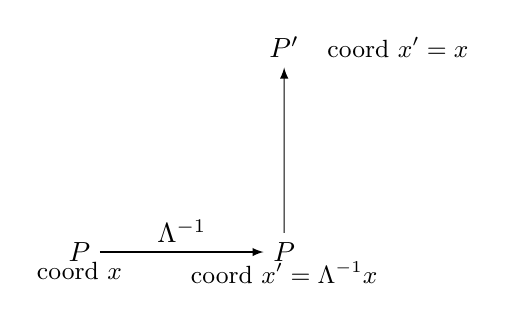
\begin{tikzpicture}[scale=1.3, baseline]
    \node at (0,0) (A) {$P$}; 
    \node at (2,0) (B) {$P$}; 
    \node at (2,2) (C) {$P'$}; 
    
    \path[->] (A) edge node[auto=left] {$\Lambda^{-1}$} (B);
    \path[->] (B) edge node[auto=left] {} (C);
    %\path[->] (A) edge node[auto=left] {z} (B);    
    
	 % \draw[<->] (A) -- (B) node[midway, below] {$xx$};
	 \node[anchor=north] at (A) {\small coord $x$};
	 \node[anchor=north] at (B) {\small coord $x'=\Lambda^{-1}x$};
	 \node[anchor=west] at (C) {\small $\quad$ coord $x'=x$};

    \end{tikzpicture}%
\end{figure}

Infinitesimal Lorentz transformation with generator $(J_V^{\mu\nu})^\rho_{\;\;\sigma}=i(\eta^{\mu\rho}\delta^\nu_\sigma-\eta^{\nu\rho}\delta^\mu_\sigma)$. Coordinates of point $P$ are $x^\rho$ - same point $P$ has coordinates $x'^\rho$ after the Lorentz trafo
\begin{align}
x'^\rho
&=x^\rho+\delta x^\rho\\
&=x^\rho-\frac{i}{2}\omega_{\mu\nu}(J_V^{\mu\nu})^\rho_{\;\;\sigma}x^\sigma
\end{align}
Local variation at fixed point $P$ (but different coordinate $x'=\Lambda x$ after traft)
\begin{align}
\delta \phi&\equiv\phi'(x')-\phi(x)
\end{align}
variation at fixed coordinate $x$ 
\begin{align}
\delta_0 \phi
&\equiv\phi'(x)-\phi(x)\\
&=\phi'(x'-\delta x)-\phi(x)\\
&=\cancel{\phi'(x')}-\partial_\mu\phi'|_{x'-\delta x}\delta x-\cancel{\phi(x)}\\
&=-\delta x^\rho\,\partial_\rho\phi'(x)\\
&=-\delta x^\rho\,\partial_\rho\phi(x)\qquad\qquad\text{why?}\\
&=\frac{i}{2}\omega_{\mu\nu}(J_V^{\mu\nu})^\rho_{\;\;\sigma}x^\sigma\,\partial_\rho\phi(x)\\
&=\frac{i}{2}\omega_{\mu\nu}(\eta^{\mu\rho}\delta^\nu_\sigma-\eta^{\mu\sigma}\delta^\nu_\rho)x^\sigma\,\partial_\rho\phi(x)\\
&=\frac{i}{2}\omega_{\mu\nu}(x^\nu\,\partial^\mu-x^\mu\,\partial^\nu)\phi(x)\\
&=\frac{i}{2}\omega_{\mu\nu}L^{\mu\nu}\phi(x)
\end{align}
where we used $\phi'(x'-\delta x)=\phi(x'-\delta x)$.

Total variation 
\begin{align}
\tilde\delta\phi_r(x)
&\equiv\phi'_r(x)-\phi_r(x)\\
&=\textcolor{red}{\phi'_r(x)-\phi'_r(x')}+\textcolor{blue}{\phi'_r(x')-\phi_r(x)}\\
&=\textcolor{red}{\frac{\partial\phi'_r(x)}{\partial x^\mu}\delta x^\mu}+\textcolor{blue}{\delta\phi_r(x)}\\
&\simeq\textcolor{red}{\frac{\partial\phi_r(x)}{\partial x^\mu}\delta x^\mu}+\textcolor{blue}{\delta\phi_r(x)}
\end{align}  

\newpage
\section{Quantization - real scalar spin 0 field (Klein Gordon field)}
\subsection{Classical}
\begin{enumerate}[a)]
\item Lagrangian for scalar field $\phi=\phi(\mathbf{x},t)$
\begin{align}
\mathcal{L}(\phi,\partial\phi)&=\frac{1}{2}g^{\mu\nu}\partial_\nu\phi\partial_\mu\phi-\frac{m^2}{2}\phi^2
\end{align}
\item Euler Lagrange equation
\begin{align}
0&=\partial_\rho\left(\frac{\partial\mathcal{L}}{\partial(\partial_\rho\phi)}\right)-\frac{\partial\mathcal{L}}{\partial\phi}\qquad\rightarrow \partial_\rho\partial^\rho\phi+m^2\phi=0
\end{align}
\item Conjugated momentum
\begin{align}
\pi(\mathbf{x},t)&=\frac{\partial\mathcal{L}}{\partial\dot{\phi}}\qquad\rightarrow \pi=\dot{\phi}
\end{align}
\item Hamilton density
\begin{align}
\mathcal{H}&=\pi\dot{\phi}-\mathcal{L}\qquad\rightarrow\mathcal{H}=\frac{1}{2}\pi^2+\frac{1}{2}(\nabla\phi)^2+\frac{m^2}{2}\phi^2
\end{align}
\item Hamiltonian
\begin{align}
H&=\int d^3x\;\frac{1}{2}\pi(x)^2-\phi(x)\triangle\phi(x)+\frac{m^2}{2}\phi(x)^2
\end{align}
\item Poisson brackets I (field and momentum)
\begin{align}
\{\phi(\mathbf{x},t),\pi(\mathbf{y},t)\}
&=\int d^3z\left(\frac{\partial\phi(\mathbf{x},t)}{\partial\phi(\mathbf{z},t)}\frac{\partial \pi(\mathbf{y},t)}{\partial\pi(\mathbf{z},t)}-\frac{\partial\phi(\mathbf{x},t)}{\partial\pi(\mathbf{z},t)}\frac{\partial \pi(\mathbf{y},t)}{\partial\phi(\mathbf{z},t)}\right)\\
&=\delta^{(3)}(\mathbf{x}-\mathbf{y})\\
\{\phi(\mathbf{x},t),\phi(\mathbf{y},t)\}&=0\\
\{\pi(\mathbf{x},t),\pi(\mathbf{y},t)\}&=0
\end{align}
\item Poisson brackets (Hamiltonian and field) II
\begin{align}
\{H,\phi(\mathbf{y},t)\}&=-\pi(\mathbf{y},t)\\
\{H,\pi(\mathbf{y},t)\}&=m^2\phi(\mathbf{y},t)-\triangle\phi(\mathbf{y})
\end{align}
\item Equations of motion
\begin{align}
\dot{\phi}(\mathbf{y},t)=-\{H,\phi\}\qquad\rightarrow\qquad\dot{\phi}(\mathbf{y},t)
&=\pi(\mathbf{y},t)\\
\dot{\pi}(\mathbf{y},t)=-\{H,\phi\}\qquad\rightarrow\qquad\dot{\pi}(\mathbf{y},t)
&=-m^2\phi(\mathbf{y},t)+\triangle\phi(\mathbf{y})\\
&\rightarrow \ddot{\phi}(\mathbf{y},t)+\triangle\phi(\mathbf{y})-m^2\phi(\mathbf{y},t)=0\\
&\rightarrow \Box\phi(\mathbf{y})+m^2\phi(\mathbf{y},t)=0
\end{align}
\item Noether theorem 
\begin{align}
\phi_i(x)\rightarrow\phi'_i(x)
&=\phi_i(x)+\delta\phi_i(x)\\
j^\rho
&=\frac{\partial\mathcal{L}}{\partial(\partial_\rho\phi_i)}\delta\phi_i-X^\rho
\quad\rightarrow\quad
\partial_\rho j^\rho=0\\
&=\frac{\partial\mathcal{L}}{\partial(\partial_\rho\phi_i)}\delta\phi_i+\mathcal{L}\delta x^\rho
\end{align}
Using Poincare invariance
\begin{align}
x'&=\Lambda x+a\simeq x+\omega x+\epsilon\\
\delta x^\alpha&\equiv x'^\alpha-x^\alpha\\
&=\omega^\alpha_{\;\beta}x^\beta+\epsilon^\alpha
\end{align}
Implied scalar field change
\begin{align}
\phi'(\Lambda x+a)&=\phi(x)\qquad\rightarrow\qquad\phi'(x)\simeq \phi(x-\omega x-\epsilon)\\
\delta\phi
&\equiv\phi'(x)-\phi(x)\\
&=\partial_\mu\phi(x)\cdot(-\delta x^\mu)\\
&=-\omega^{\mu\nu}x_\nu\partial_\mu\phi(x)-\epsilon^\mu\partial_\mu\phi(x)
\end{align}
Implied Langrangian (scalar) change
\begin{align}
\mathcal{L}'(\Lambda x+a)
&=\mathcal{L}(x)\qquad\rightarrow\qquad\mathcal{L}'(x)=\mathcal{L}(x-\omega x-\epsilon)\\
\delta\mathcal{L}(x)
&\equiv\mathcal{L}'(x)-\mathcal{L}(x)\\
&=(-\delta x^\mu)\;\partial_\mu\mathcal{L}\\
&=-\partial_\mu(\delta x^\mu\,\mathcal{L})+\mathcal{L}\partial_\mu(\delta x^\mu)\\
&=\partial_\mu(-\omega^\mu_{\;\nu} x^\nu\mathcal{L}-\epsilon^\mu \mathcal{L})\\
&\rightarrow X^\mu=-\omega^\mu_{\;\nu} x^\nu\mathcal{L}-\epsilon^\mu \mathcal{L}=-\mathcal{L}\delta x^\mu
\end{align}
Now we can calculate the Noether current
\begin{align}
j^\rho=(\partial^\rho\phi)\left[-\omega^{\mu\nu}x_\nu\partial_\mu\phi-\epsilon^\mu\partial_\mu\phi\right]+\omega^{\mu\nu}x_\nu\mathcal{L}+\epsilon^\rho\mathcal{L}
\end{align}
Translational invariance ($\sim-\epsilon^\mu$ coeff)
\begin{align}
T^\rho_{\;\mu}&=(\partial^\rho\phi)(\partial_\mu\phi)-g^\rho_{\;\mu}\mathcal{L}\\
T^{\rho\mu}&=(\partial^\rho\phi)(\partial^\mu\phi)-g^{\rho\mu}\mathcal{L}
\end{align}
Lorenz invariance ($\sim\frac{1}{2}\omega^{\mu\nu}$ coeff)
\begin{align}
\mathcal{M}^\rho_{\;\mu\nu}&=(\partial^\rho\phi)(x_\mu\partial_\nu-x_\nu\partial_\mu)\phi+(g^\rho_{\;\mu}x_\nu-g^\rho_{\;\nu}x_\mu)\mathcal{L}\\
\mathcal{M}^{\rho\mu\nu}&=(\partial^\rho\phi)(x^\mu\partial^\nu-x^\nu\partial^\mu)\phi+(g^{\rho\mu}x^\nu-g^{\rho\nu}x^\mu)\mathcal{L}\\
&=T^{\rho\nu}x^\mu-T^{\rho\mu}x^\nu
\end{align}
Conserved quantities (with $\partial^\mu\phi=g^{\mu\nu}\partial_\nu\phi$ we see $\partial^0\phi=g^{0\nu}\partial_\nu\phi=g^{00}\partial_0\phi=\partial_0\phi\equiv\dot{\phi}$
\begin{align}
P^\mu
&=\int d^3x\;T^{0\mu}\\
&=\int d^3x\;(\dot\phi\partial^\mu\phi)-\frac{1}{2}g^{0\mu}(\partial_\alpha\phi\partial^\alpha\phi-m^2\phi^2)\\
\text{energy}\rightarrow P^0&=\frac{1}{2}\int d^3x\;\dot{\phi}^2+(\nabla\phi)^2+m^2\phi^2\\
\text{momentum}\rightarrow P^k&=\int d^3x\;\dot{\phi}(\partial^k\phi)
\end{align}
\begin{align}
J^{\mu\nu}
&=\int d^3x\;M^{0\mu\nu}\\
&=\int d^3x\;(T^{0\nu}x^\mu-T^{0\mu}x^\nu)\\
\text{rotation}\rightarrow J^{ik}
&=\int d^3x\;(T^{0k}x^i-T^{0i}x^k)\\
&=\int d^3x\;\dot{\phi}(x^i\partial^k-x^k\partial^i)\phi\\
\text{angular momentum}\rightarrow J_j
&\equiv\frac{1}{2}\epsilon_{jik}J^{ik}\\
&=\frac{1}{2}\int d^3x\;(\epsilon_{jik}T^{0k}x^i-\epsilon_{jik}T^{0i}x^k)\\
&=\int d^3x\;(\epsilon_{jik}x^iT^{0k})\\
&=\int d^3x\;(\mathbf{x}\times \mathbf{\mathcal{P}})\\
\text{boost}\rightarrow J^{0k}
&=\int d^3x\;\dot{\phi}(x^0\partial^k-x^k\partial^0)\phi+x^k\mathcal{L}
\end{align}

\end{enumerate}
\subsection{Quantized}
\begin{enumerate}[a)]
\item Quantization (obtained from Poisson brackets I)
\begin{align}
[\hat{\phi}(\mathbf{x},t),\hat{\phi}(\mathbf{y},t)]&=0\\
[\hat{\phi}(\mathbf{x},t),\hat{\pi}(\mathbf{y},t)]&=i\delta^{(3)}(\mathbf{x}-\mathbf{y})\\
[\hat{\pi}(\mathbf{x},t),\hat{\pi}(\mathbf{y},t)]&=0\\
\mathcal{H}=\mathcal{H}(\hat{\phi},\hat{\pi})
\end{align}
\item Time evolution in the Heisenberg picture (calculated from $\hat{\mathcal{H}}, \hat{\phi}$ and $\hat{\pi}$)
\begin{align}
\dot{\hat{\phi}}(x)&=i[\hat{H},\hat{\phi}(x)]=\hat{\pi}(x)\\
\dot{\hat{\pi}}(x)&=i[\hat{H},\hat{\pi}(x)]=\triangle\hat{\phi}(x)-m^2\hat{\phi}(x)
\end{align} 
\item Equations of motion (operator identity)
\begin{align}
(\Box+m^2)\hat{\phi}(x)=0
\end{align}
\item (free) field operators (Heisenberg picture) are derived as ansatz to solve the equations of motion
\begin{align}
\hat\phi(x)
&=\int \frac{d^3p}{(2\pi)^3}\frac{1}{2E_\mathbf{p}}
(\hat{a}_\mathbf{p}e^{-ipx}
+\hat{a}_\mathbf{p}^\dagger e^{ipx})\\
\hat\phi(\mathbf{x},t)
&=\int \frac{d^3p}{(2\pi)^3}\frac{1}{2E_\mathbf{p}}
(\hat{a}_\mathbf{p}e^{-i(E_pt-\mathbf{p\cdot x})}
+\hat{a}_\mathbf{p}^\dagger e^{i(E_pt-\mathbf{p\cdot x})})
\end{align}
\item Commutators of the ladder operators
\begin{align}
[a_\mathbf{p},a_\mathbf{q}]&=0\\
[a_\mathbf{p},a^\dagger_\mathbf{q}]&=(2\pi)^32E_\mathbf{p}\delta^{(3)}(\mathbf{p}-\mathbf{q})\\
[a^\dagger_\mathbf{p},a^\dagger_\mathbf{q}]&=0
\end{align}
Hamiltonian
\begin{align}
\hat{H}
&=\frac{1}{2}\int d^3x\;\hat\pi(x)^2+(\nabla\hat\phi(x))^2+m^2\hat\phi(x)^2\\
&=\int d^3\tilde{p}\;E_\mathbf{p}
\hat{a}^\dagger_\mathbf{p}\hat{a}_\mathbf{p}
+\frac{1}{2}\int d^3p\delta^{(3)}(0)
\end{align}
The calculation of the commutator is now simple
\begin{align}
[\hat{H},\hat{a}^\dagger_\mathbf{p}]&=E_\mathbf{q}\hat{a}^\dagger_\mathbf{q}
\end{align}

\item Conserved quantities
\begin{align}
\hat{P}^0
&=\frac{1}{2}\int d^3x\;\hat{\pi}^2+(\nabla\hat{\phi})^2+m^2\hat{\phi}^2\\
&=\int d^3\tilde{p}\;E_\mathbf{p}
\hat{a}^\dagger_\mathbf{p}\hat{a}_\mathbf{p}
+\frac{1}{2}\int d^3p\,\delta^{(3)}(0)\\
\hat{P}^k
&=\int d^3x\;\hat{\pi}(\partial^k\hat{\phi})\\
&=\int d^3x\, \mathbf{p}\hat{a}_\mathbf{p}^\dagger \hat{a}_\mathbf{p}
\end{align}
\begin{align}
\hat{J}^{ik}
&=\int d^3x\;\dot{\hat{\phi}}(x^i\partial^k-x^k\partial^i)\hat{\phi}\\
&=\int d^3x\;\hat{\pi}(x^i\partial^k-x^k\partial^i)\hat{\phi}\\
\hat{J}^{0k}
&=\int d^3x\;\dot{\hat{\phi}}(x^0\partial^k-x^k\partial^0)\hat{\phi}+\frac{1}{2}x^k(\partial^\mu\hat{\phi}\partial_\mu\hat{\phi}-m^2\hat{\phi}^2)\\
&=\int d^3x\;(x^0\dot{\hat{\phi}}\partial^k\hat{\phi}-x^k\dot{\hat{\phi}}^2)+\frac{1}{2}x^k(\dot{\hat\phi}^2-(\partial_k\hat{\phi})^2-m^2\hat{\phi}^2)\\
&=\int d^3x\;x^0\dot{\hat{\phi}}\partial^k\hat{\phi}+\frac{1}{2}x^k(-\dot{\hat\phi}^2-(\partial_k\hat{\phi})^2-m^2\hat{\phi}^2)\\
&=\int d^3x\;x^0\hat{\pi}\partial^k\hat{\phi}+\frac{1}{2}x^k(-\hat{\pi}^2-(\partial_k\hat{\phi})^2-m^2\hat{\phi}^2)
\end{align}

\item Commutation relations
\begin{align}
[P^\mu,P^\nu]&=\\
[P^\mu,J^{\rho\sigma}]&=
\end{align}

\item Commutation relations
\begin{align}
[\hat{P}^k,\hat{\phi}(y)]
&=\int d^3x\;[\hat{\pi}(x)(\partial^k\hat{\phi}(x)),\hat{\phi}(y)]\\
&=\int d^3x\;\hat{\pi}(x)(\partial^k\hat{\phi}(x))\hat{\phi}(y)-\hat{\phi}(y)\hat{\pi}(x)(\partial^k\hat{\phi}(x))\\
&=\int d^3x\;\hat{\pi}(x)(\partial^k\hat{\phi}(x))\hat{\phi}(y)-\hat{\pi}(x)\hat{\phi}(y)(\partial^k\hat{\phi}(x))+i\int d^3x\;\delta^{(3)}(\mathbf{x}-\mathbf{y})\partial^k\hat{\phi}(x)\\
&=i\partial^k\hat{\phi}(y)\\
[\hat{P}^0,\hat{\phi}(y)]&=\\
\end{align}
\begin{align}
[\hat{J}^{ik},\hat{\phi}(y)]
&=\int d^3x\;[\hat{\pi}(x)(x^i\partial^k-x^k\partial^i)\hat{\phi}(x),\hat{\phi}(y)]\\
&=\int d^3x\;x^i[\hat{\pi}(x)(\partial^k\hat{\phi}(x)),\hat{\phi}(y)]-x^k[\hat{\pi}(x)(\partial^i\hat{\phi}(x)),\hat{\phi}(y)]\\
&=\int d^3x\,\left(-x^i\delta^{(3)}(\mathbf{x}-\mathbf{y})(\partial^k\hat{\phi}(x))+x^k\delta^{(3)}(\mathbf{x}-\mathbf{y})(\partial^i\hat{\phi}(x))\right)\\
&=-i(y^i\partial^k-y^k\partial^i)\hat{\phi}(y)\\
[\hat{J}^{0k},\hat{\phi}(y)]&=\\
[P^\mu,a^\dagger_\mathbf{p}]&=p^\mu a^\dagger_\mathbf{p}\\
[J^{\rho\sigma},a^\dagger_\mathbf{p}]&=\\
\end{align}
Then
\begin{align}
\left(1-\frac{i}{2}\omega_{\mu\nu}\hat{J}^{\mu\nu}\right)\hat{\phi}(x)\left(1+\frac{i}{2}\omega_{\mu\nu}\hat{J}^{\mu\nu}\right)=
\end{align}




\item Hilbert space
\begin{itemize}
\item as commutator algebra for $\hat{a}$ and $\hat{a}^\dagger$ is as for harmonic oscillator we utilize the same Hilbert space (with $E_\mathbf{p}=\sqrt{m^2+\mathbf{p}^2}$ and therefore $p=(E_\mathbf{p},\mathbf{p})=(\sqrt{m^2+\mathbf{p}^2},\mathbf{p})$ - so $\mathbf{p}$ defines $p$)
\begin{align}
a_\mathbf{p}|0\rangle&\equiv0\\
|p\rangle
&\equiv \sqrt{2E_\mathbf{p}}a^\dagger_\mathbf{p}|0\rangle\\
\langle p|p'\rangle&=(2\pi)^3 2E_\mathbf{p}\delta^3(\mathbf{p}-\mathbf{p}')\\
\hat{P}^\mu|p\rangle
&=\sqrt{2E_\mathbf{p}}\hat{P}^\mu a^\dagger_\mathbf{p}|0\rangle
=\sqrt{2E_\mathbf{p}}(a^\dagger_\mathbf{p}\hat{P}^\mu+p^\mu a^\dagger_\mathbf{p} )|0\rangle
=p^\mu|p\rangle\\
\hat{P}^\mu|p_1,...,p_n\rangle
&=(p^\mu_1+...+p^\mu_n)|p_1,...,p_n\rangle\\
U(\Lambda)|p\rangle
&=|\Lambda p\rangle
=\sqrt{2E_{\Lambda\mathbf{p}}}a^\dagger_{\Lambda\mathbf{p}}|0\rangle\\
U(\Lambda)|p_1,p_2,...\rangle&=|\Lambda p_1,\Lambda p_2,...\rangle\\
U(\Lambda)a^\dagger_\mathbf{p}U^{-1}(\Lambda)
&=\sqrt{\frac{E_{\Lambda\mathbf{p}}}{E_\mathbf{p}}}a^\dagger_{\Lambda\mathbf{p}}\\
U(\Lambda)a_\mathbf{p}U^{-1}(\Lambda)
&=\sqrt{\frac{E_{\Lambda\mathbf{p}}}{E_\mathbf{p}}}a_{\Lambda\mathbf{p}}\\
\end{align}

\end{itemize}
\end{enumerate}

\newpage
\section{Quantization - complex scalar spin 0 field}
\subsection{Classical}
\begin{enumerate}[a)]
\item Lagrangian 

For complex scalar field $\varphi=\varphi(\mathbf{x},t)=\varphi_1(\mathbf{x},t)+i\varphi_2(\mathbf{x},t)$. The two real (fundamental) fields can be chosen as $\varphi_1$ and $\varphi_2$ or as $\varphi$ and $\varphi^*$
\begin{align}
\mathcal{L}(\varphi,\varphi^*,\partial\varphi,\partial\varphi^*)
&=(\partial_\mu\varphi^*)(\partial^\mu\varphi)-m^2\varphi^*\varphi
\end{align}

\item Euler Lagrange equation
\begin{align}
\partial_\mu\partial^\mu\varphi^*+m^2\varphi^*&=0\\
\partial_\mu\partial^\mu\varphi+m^2\varphi&=0
\end{align}
\item Conjugated momentum
\begin{align}
\pi&=\frac{\partial\mathcal{L}}{\partial(\partial_0\varphi)}=\partial^0(\varphi^*)\qquad\rightarrow \pi=\partial^0{\varphi^*}\\
\pi^*&=\frac{\partial\mathcal{L}}{\partial(\partial_0\varphi^*)}=\partial^0(\varphi)\qquad\rightarrow \pi^*=\partial^0{\varphi}=(\partial^0{\varphi^*})^*\equiv(\pi)^*
\end{align}
\item Hamiltonian density
\item Hamiltonian
\begin{align}
H=\int d^3x\left(\pi^*\pi+(\nabla\varphi^*)\cdot(\nabla\varphi)+m^2\varphi^*\varphi\right)
\end{align}
\item Poisson brackets I (field and momentum)
\item Poisson brackets II (Hamiltonian and field)
\item Equations of motion
\item Noether theorem 
\begin{align}
\phi_i(x)\rightarrow\phi'_i(x)
&=\phi_i(x)+\delta\phi_i(x)\\
j^\rho
&=\frac{\partial\mathcal{L}}{\partial(\partial_\rho\phi_i)}\delta\phi_i-X^\rho
\quad\rightarrow\quad
\partial_\rho j^\rho=0\\
&=\frac{\partial\mathcal{L}}{\partial(\partial_\rho\phi_i)}\delta\phi_i+\mathcal{L}\delta x^\rho
\end{align}
\begin{itemize}
\item Poincare invariance leads to energy, momentum and angular momentum conservation
\item One more internal symmetry (meaning $\delta x=0$)
\begin{align}
\varphi'(x)&=e^{-i\alpha}\varphi(x)\simeq(1-i\alpha)\varphi(x)\\
\delta\varphi(x)
&\equiv\varphi'(x)-\varphi(x)\\
&\simeq-i\varphi(x)\delta\alpha\\
\delta\varphi^*(x)
&\simeq+i\varphi^*(x)\delta\alpha
\end{align}
then
\begin{align}
j
&=(\partial^\mu\varphi^*)\delta\varphi+(\partial^\mu\varphi)\delta\varphi^*\\
&=i\alpha[-(\partial^\mu\varphi^*)\varphi+(\partial^\mu\varphi)\varphi^*]
\end{align}
\end{itemize}

\end{enumerate}


\subsection{Quantized}

\newpage
\section{Quantization - spin-\sfrac{1}{2} field (Dirac field)} 
\subsection{Prelim}
Pauli matrices
\begin{align}
\textcolor{red}{\sigma_0=\left(\begin{array}{cc}1&0\\0&1\end{array}\right)}
\quad
\sigma_1&=\left(\begin{array}{cc}0&1\\1&0\end{array}\right)
\quad
\sigma_2=\left(\begin{array}{cc}0&-i\\i&0\end{array}\right)
\quad
\sigma_3=\left(\begin{array}{cc}1&0\\0&-1\end{array}\right)\\
&\rightarrow[\sigma_j,\sigma_k]=2i\epsilon_{jkl}\sigma_l\\
&\rightarrow\{\sigma_j,\sigma_k\}=2\delta_{jk}\sigma_0
\end{align}
and we also define 
\begin{align}
\sigma^\mu&=(\sigma_0,\mathbf{\sigma}_k)\\
\tilde{\sigma}^\mu&=(\sigma_0,-\mathbf{\sigma}_k)
\end{align}
General Dirac matrices
\begin{align}
\{\gamma^\mu,\gamma^\nu\}&=2g^{\mu\nu} 1_{n\times n}\qquad\text{Dirac algebra}\\
&\rightarrow (\gamma^0)^2=+1_{n\times n}\\
&\rightarrow (\gamma^k)^2=-1_{n\times n}\\
S^{\mu\nu}&\equiv\frac{i}{4}[\gamma^\mu,\gamma^\nu]\qquad \text{$n$-dimensional rep. of Lorentz algebra because ...}\\
&\rightarrow [S^{\mu\nu},S^{\rho\sigma}]=i(
g^{\nu\rho}S^{\mu\sigma}
-g^{\mu\rho}S^{\nu\sigma}
-g^{\nu\sigma}S^{\mu\rho}
+g^{\mu\sigma}S^{\nu\rho})
\end{align}
Theorem: There is {\bf exactly one irreducible representation} of the Dirac matrices and the irrep is 4-dimensional.

\subsubsection{Representations of the $\gamma$-matrices}
\begin{enumerate}
\item {\bf Weyl/chiral basis/High-energy representation} - for 4d-Minkowski space SO(1,3) - needs 4 $\gamma$ matrices which are coincidentally $4\times4$ matrices
\begin{align}
\gamma^0&=\left(\begin{array}{cc}0 &1_{2\times2}\\1_{2\times2} &0\end{array}\right)
\qquad
\gamma^k=\left(\begin{array}{cc}0 & \sigma_k\\ -\sigma_k &0\end{array}\right)\\
&\rightarrow\gamma^\mu=\left(\begin{array}{cc}0 & \sigma^\mu\\ \tilde{\sigma}^\mu &0\end{array}\right)\\
&\rightarrow S^{0k}\equiv\frac{i}{4}[\gamma^0,\gamma^k]=\frac{i}{2}\gamma^0\gamma^k=-\frac{i}{2}\left(\begin{array}{cc}\sigma_k &0\\0 &-\sigma_k\end{array}\right)\\
&\rightarrow S^{jk}\equiv\frac{i}{4}[\gamma^j,\gamma^k]=\frac{1}{2}\epsilon^{jkl}\left(\begin{array}{cc}\sigma_l &0\\0 &\sigma_l\end{array}\right)
\end{align}
we see that in the Weyl basis $(\gamma^0)^\dagger=\gamma^0, (\gamma^k)^\dagger=-\gamma^k$ and $(\gamma^0)^2=1_{4\times4}$ and $(\gamma^k)^2=-1_{4\times4}$.

\item {\bf Dirac basis representation}
\begin{align}
\gamma^0&=\left(\begin{array}{cc}1_{2\times2}&0\\0&-1_{2\times2}\end{array}\right)\qquad
\gamma^k=\left(\begin{array}{cc}0 & \sigma_k\\ -\sigma_k &0\end{array}\right)
\end{align}
we see that in the Dirac basis $(\gamma^0)^\dagger=\gamma^0, (\gamma^k)^\dagger=-\gamma^k$ and $(\gamma^0)^2=1_{4\times4}$ and $(\gamma^k)^2=-1_{4\times4}$.
\end{enumerate}

\subsubsection{Notation}
In the Weyl representation we define
\begin{align}
\tilde{V}&\equiv\sigma^\mu V_\mu=\sigma^\mu g_{\mu\nu}V^\nu=\left(\begin{array}{cc}
V_0+V_3 & V_1-iV_2\\
V_1+iV_2 & V_0-V_3
\end{array}\right)\\
&\rightarrow\det(\sigma^\mu V_\mu)=V_0^2-V_3^2-V_1^2-V_2^2=g^{\mu\nu}V_\mu V_\nu \\
\slashed{p}&\equiv\gamma^\mu p_\mu
=\left(\begin{array}{cc}0 & \sigma^\mu p_\mu\\ \tilde{\sigma}^\mu p_\mu &0\end{array}\right)\\
&\rightarrow\slashed{p}\slashed{p}=\gamma^\mu\gamma^\nu p_\mu p_\nu=\frac{1}{2}(\gamma^\mu\gamma^\nu+\gamma^\nu\gamma^\mu)p_\mu p_\nu=g^{\mu\nu}p_\mu p_\nu=p^2 1_{4\times4}
\end{align}

\subsubsection{Dirac equation}
With the Dirac spinor
\begin{align}
\psi=\left(\begin{matrix}\phi\\ \chi\end{matrix}\right)
\end{align}
we can write the Dirac equation (which then implies Klein-Gordon equation)
\begin{align}
(\slashed{p}-mc)
\left(\begin{matrix}\phi\\ \chi\end{matrix}\right)=0\\
\rightarrow(\slashed{p}+mc)(\slashed{p}-mc)
\left(\begin{matrix}\phi\\ \chi\end{matrix}\right)=0\\
\rightarrow(p^2-m^2c^2)
\left(\begin{matrix}\phi\\ \chi\end{matrix}\right)=0
\end{align}
In components this means
\begin{align}
\textcolor{blue}{(\sigma^\mu p_\mu)\chi}
&=\textcolor{purple}{mc\phi}\\
\textcolor{blue}{(\tilde{\sigma}^\mu p_\mu)\phi}&=\textcolor{purple}{mc\chi}
\end{align}

\subsubsection{Lorentz Transformation}
\begin{itemize}
\item Observe: For real $\xi^\mu$ the $2\times2$ matrices $\tilde{\xi}=\sigma^\mu \xi_\mu$ (see definition above) as well as $A(\sigma^\mu \xi_\mu)A^\dagger$ are self-adjoint and we can write (assuming $\eta_\nu\equiv\Lambda(A)\xi_\mu$ depends linearly on $\xi$ - where $\Lambda(A)$ is a $4\times4$ matrix)
\begin{align}
\textcolor{red}{A(\sigma^\mu \xi_\mu)A^\dagger} = \sigma^\mu \eta_\mu = \textcolor{red}{\sigma^\mu (\Lambda(A)\xi_\mu)}
\end{align}
\item $\Lambda(A)$ is a representation of $A$ because of 
\begin{align}
\rightarrow \sigma^\mu(\Lambda(A_1A_2)\xi)_\mu=A_1A_2(\sigma^\mu\xi_,u)(A_1A_2)^\dagger=...=\sigma^\mu(\Lambda(A_1)\Lambda(A_2)\xi)_\mu
\end{align}
\item If $A\in \text{SL}(2,\mathbb{C}$) - meaning $\det A = 1$ and 
\begin{align}
\xi^\mu\xi_\mu=\det(\sigma^\mu\xi_\mu)=\det(A\sigma^\mu\xi_\mu A^\dagger)=\det(\sigma^\mu(\Lambda(A)\xi)_\mu)=(\Lambda(A)\xi)^\mu(\Lambda(A)\xi)_\mu
\end{align}
then $\Lambda(A)$ is Lorentz Transformation for each $A\in$ SL(2,$\mathbb{C}$) - and also a 4-dimensional representation of SL(2,$\mathbb{C}$)
\item For a LT invariant theory the LT transformed spinors must also fulfill the Dirac equation: Now consider LT
\begin{align}
x'=\Lambda(A)x+a,\qquad p'=\Lambda(A)p
\end{align}
then we use the Dirac equation (in the LT transformed system) and the identity above
\begin{align}
\textcolor{blue}{(\sigma^\mu p'_\mu)\chi'}=\textcolor{red}{(\sigma^\mu \Lambda(A)p_\mu)}\chi'
=\textcolor{red}{A(\sigma^\mu p_\mu)A^\dagger}\chi'
&\overset{!}{=}\textcolor{purple}{mc\phi'}
\\
\textcolor{blue}{(\tilde{\sigma}^\mu p'_\mu)\phi'}=\textcolor{red}{(\tilde{\sigma}^\mu \Lambda(A)p_\mu)}\phi'
=\textcolor{red}{A(\tilde{\sigma}^\mu p_\mu)A^\dagger}\phi'
&\overset{!}{=}\textcolor{purple}{mc\chi'}
\end{align}
substituting $\chi'(x')={A^\dagger}^{-1}\chi(x)$ and $\phi'(x')=A\phi(x)$
\begin{align}
\textcolor{red}{A(\sigma^\mu p_\mu)A^\dagger}\chi'
&\overset{!}{=}\textcolor{purple}{mc\phi'}
\quad\rightarrow\quad
A(\sigma^\mu p_\mu)\chi(x)=Amc\phi
\\
\textcolor{red}{A(\tilde{\sigma}^\mu p_\mu)A^\dagger}\phi'
&\overset{!}{=}\textcolor{purple}{mc\chi'}\quad\rightarrow\quad
A(\tilde{\sigma}^\mu p_\mu)\phi(x)=Amc\chi
\end{align}
we recover the Dirac equation. So we conclude that Dirac spinors transform like
\begin{align}
\psi'(x')
=\left(\begin{matrix}
\phi'(x')\\ \chi'(x')
\end{matrix}\right)
=\left(\begin{matrix}
A & 0\\
0 & {A^\dagger}^{-1}
\end{matrix}\right)
\left(\begin{matrix}
\phi(x)\\ \chi(x)
\end{matrix}\right)
\equiv S(A)\psi(x)
\end{align}
where ($(A^\dagger)^{-1}=(A^{-1})^\dagger$)
\begin{align}
S(A)=\left(\begin{matrix}
A & 0\\
0 & {A^\dagger}^{-1}
\end{matrix}\right),\qquad
S(A)^{-1}=\left(\begin{matrix}
A^{-1} & 0\\
0 & A^\dagger
\end{matrix}\right),\qquad
S(A)^\dagger=\left(\begin{matrix}
A^\dagger & 0\\
0 & A^{-1}
\end{matrix}\right)
\end{align}
\item Then
\begin{align}
S(A)(\gamma^\mu p_\mu)S(A)^{-1}
&=\left(\begin{matrix}
A & 0\\0&{A^\dagger}^{-1}
\end{matrix}
\right)
\left[p_0\left(\begin{matrix}
0 & \sigma_0\\\sigma_0&0
\end{matrix}\right)+p_k\left(\begin{matrix}
0 & \sigma_k\\-\sigma_k&0
\end{matrix}\right)+\right]
\left(\begin{matrix}
A^{-1} & 0\\0&A^\dagger
\end{matrix}
\right)\\
&=\left(\begin{matrix}
0 & A(\sigma^\mu p_\mu)A^\dagger\\
{A^\dagger}^{-1}(\tilde{\sigma}^\mu p_\mu)A^{-1} &0
\end{matrix}
\right)\\
&=...\\
&=\Lambda^{-1}(A)^\mu_{\,\nu}\gamma^\nu\, p_\mu
\end{align}
or equivalently:
\begin{align}
S(A)^{-1}\gamma^\mu S(A)
&=\Lambda^\mu_{\,\nu}\gamma^\nu
\end{align}
\item And
\begin{align}
\gamma^0S^\dagger\gamma^0
=\left(
\begin{matrix}
0&\sigma_0\\ \sigma_0&0
\end{matrix}
\right)
\left(
\begin{matrix}
A^\dagger&0\\ 0&A^{-1}
\end{matrix}
\right)
\left(
\begin{matrix}
0&\sigma_0\\ \sigma_0&0
\end{matrix}
\right)
=\left(
\begin{matrix}
A^{-1}&0\\ 0&A^\dagger
\end{matrix}
\right)
=S^{-1}
\end{align}
\item Consider parity transformation $P$
\begin{align}
x'=Px=(x^0,-\vec{x}),&\qquad p'=Pp=(p^0,-\vec{p})\\
&\rightarrow\sigma^\mu p'_\mu=\tilde{\sigma}^\mu p_\mu\\
&\rightarrow\tilde{\sigma}^\mu p'_\mu=\sigma^\mu p_\mu
\end{align}
then
\begin{align}
\psi'(x')
=\left(\begin{matrix}
\phi'(x')\\ \chi'(x')
\end{matrix}\right)
=\left(\begin{matrix}
0 & \sigma_0\\
\sigma_0 & 0
\end{matrix}\right)
\left(\begin{matrix}
\phi(x)\\ \chi(x)
\end{matrix}\right)
\equiv S(P)\psi(x)
\end{align}
with
\begin{align}
S(P)=\left(\begin{matrix}
0 & \sigma_0\\
\sigma_0 & 0
\end{matrix}\right)
=\gamma^0
\end{align}
then
\begin{align}
S(P)^{-1}\gamma^0S(P)&=\gamma^0\gamma^0\gamma^0=\gamma^0\\
S(P)^{-1}\gamma^kS(P)&=\gamma^0\gamma^k\gamma^0\\
&=(2g^{0k}1_{n\times n}-\gamma^k\gamma^0)\gamma^0\\
&=-\gamma^k\underbrace{\gamma^0\gamma^0}_{=1}\\
&=-\gamma^k
\end{align}
\item Conjugate spinor 
\begin{align}
\bar{\psi}(x)
&\equiv\psi^\dagger(x)\gamma^0\\
&=(\phi^*(x)\; \chi^*(x))\left(\begin{matrix}
0 & \sigma_0\\
\sigma_0 & 0
\end{matrix}\right)=(\chi^*(x)\; \phi^*(x))\\
\bar{\psi}'(x')
&=(S(A)\psi(x))^\dagger\gamma^0\\
&=\psi^\dagger(x) S(A)^\dagger\gamma^0\\
&=\psi^\dagger(x) \gamma^0 S(A)^{-1}\\
&=\bar{\psi}(x) S(A)^{-1}
\end{align}
\item $\gamma_5=i\gamma^0\gamma^1\gamma^2\gamma^3$
\begin{align}
P_+&=\frac{1+\gamma_5}{2},\qquad P_-=\frac{1-\gamma_5}{2}\\
&\rightarrow P_+ + P_-=1\\
&\rightarrow P_\pm^2=1\\
&\rightarrow P_\pm^\dagger=P_\pm\\
&\rightarrow P_+\left(
\begin{matrix}
\phi\\
\chi
\end{matrix}
\right)
=\left(\begin{matrix}
0\\
\chi
\end{matrix}
\right),
\qquad
P_-\left(
\begin{matrix}
\phi\\
\chi
\end{matrix}
\right)
=\left(\begin{matrix}
\phi\\
0
\end{matrix}
\right)
\end{align}

\end{itemize}



For the {\bf Weyl} and the {\bf Dirac} representation we can can show (using the hermiticity relations)
\begin{align}
\gamma^0\gamma^\mu\gamma^0=(\gamma^\mu)^\dagger
\end{align}
In general
\begin{align}
[\gamma^\mu,S^{\rho\sigma}]&=(J^{\rho\sigma})^\mu_{\;\nu}\gamma^\nu\\
\gamma^0S^{\rho\sigma}\gamma^0&=(S^{\rho\sigma})^\dagger
\end{align}
And
\begin{align}
\bar{\Psi}&\equiv\Psi^\dagger\gamma^0\\
\Psi&\rightarrow S(\Lambda)\Psi\qquad\text{Dirac spinor}\\
\bar{\Psi}&\rightarrow \bar{\Psi}S^{-1}(\Lambda)\\
x'&=\Lambda x+a\simeq (1+\omega)x+\epsilon\\
\Psi'(\Lambda x+a)
&=S(\Lambda)\Psi(x)\qquad\text{Dirac spinor field}\\
\rightarrow \Psi'(x)
&=\Psi(x)-\frac{i}{2}\omega_{\rho\sigma}\left(S^{\rho\sigma}+L^{\rho\sigma}\right)\Psi(x)-\epsilon^\mu\partial_\mu\Psi(x)\qquad\text{with}\qquad L^{\rho\sigma}=i(x^\rho\partial^\sigma-x^\sigma\partial^\rho)
\end{align}

\subsection{Classical}
\begin{enumerate}[a)]
\item Lagrangian with $\bar{\Psi}=\Psi^\dagger\gamma^0$
\begin{align}
\mathcal{L}(\Psi,\partial\Psi,\bar{\Psi},\partial\bar{\Psi})
&=\bar{\Psi}(i\gamma^\mu\partial_\mu-m)\Psi
\end{align}
\item Euler-Lagrange equation
\begin{align}
\bar{\Psi}:\quad&\rightarrow\quad(i\gamma^\mu\partial_\mu-m)\Psi(x)=0\\
\Psi:\quad&\rightarrow\quad(m+i\gamma^\mu\partial_\mu)\bar{\Psi}(x)=0
\end{align}
\item Conjugated momenta
\begin{align}
\pi(x)&=\frac{\partial\mathcal{L}}{\partial\dot{\Psi}}=i\gamma^0\bar{\Psi}(x)=i\Psi^\dagger(x)\\
\bar{\pi}(x)&=0
\end{align}
\item Hamiltonian
\begin{align}
\mathcal{H}
&=\pi\Psi+\bar{\pi}\bar{\Psi}-\mathcal{L}\\
&=\pi(x)\gamma^0\gamma^k\partial_k\Psi(x)+m\bar{\Psi}\Psi
\end{align}
\item Poisson brackets
\begin{align}
\{\Psi(\mathbf{x},t),\pi(\mathbf{y},t)\}&=\delta^{(3)}(\mathbf{x}-\mathbf{y})\\
\{\Psi(\mathbf{x},t),\Psi(\mathbf{y},t)\}&=0\\
\{\pi(\mathbf{x},t),\pi(\mathbf{y},t)\}&=0
\end{align}

\item Noether theorem
\begin{align}
\phi_i(x)\rightarrow\phi'_i(x)
&=\phi_i(x)+\delta\phi_i(x)\\
j^\rho
&=\frac{\partial\mathcal{L}}{\partial(\partial_\rho\phi_i)}\delta\phi_i-X^\rho
\quad\rightarrow\quad
\partial_\rho j^\rho=0
\end{align}
with Poincare invariance
\begin{align}
\mathcal{L}&=\bar{\psi}(i\gamma^\mu\partial_\mu-m)\Psi\\
x'&=\Lambda x+a\simeq x+\omega x+\epsilon
\end{align}
Implied spinor field change
\begin{align}
\Psi'(\Lambda x+a)&=S(\Lambda)\Psi(x)\qquad\rightarrow\qquad\Psi'(x)\simeq S(\Lambda)\Psi(x-\omega x-\epsilon)\\
\delta\Psi
&\equiv\Psi'(x)-\Psi(x)\\
&=-\frac{i}{2}\omega_{\rho\sigma}\left(S^{\rho\sigma}+L^{\rho\sigma}\right)\Psi(x)-\epsilon^\mu\partial_\mu\Psi(x)\qquad\text{with}\;L^{\rho\sigma}=i(x^\rho\partial^\sigma-x^\sigma\partial^\rho)
\end{align}
Implied Langrangian (scalar) change
\begin{align}
\mathcal{L}'(\Lambda x+a)
&=\mathcal{L}(x)\qquad\rightarrow\qquad\mathcal{L}'(x)=\mathcal{L}(x-\omega x-\epsilon)\\
\delta\mathcal{L}(x)
&\equiv\mathcal{L}'(x)-\mathcal{L}(x)\\
&=\partial_\mu(-\omega^\mu_{\;\nu} x^\nu\mathcal{L}-\epsilon^\mu \mathcal{L})\\
&\rightarrow X^\mu=-\omega^\mu_{\;\nu} x^\nu\mathcal{L}-\epsilon^\mu \mathcal{L}
\end{align}
Now we can calculate the Noether current
\begin{align}
j^\mu&=\bar{\Psi}i\gamma^\rho\left(\epsilon^\mu\partial_\mu\Psi-\frac{i}{2}\omega_{\mu\nu}(S^{\mu\nu}+L^{\mu\nu})\Psi\right)+\epsilon^\rho\mathcal{L}+\omega^{\rho\sigma}x_\sigma\mathcal{L}
\end{align}
Translational invariance ($\sim\epsilon^\mu$ coeff)
\begin{align}
T^\rho_{\;\mu}=\bar{\Psi}i\gamma^\rho\partial_\mu\Psi-g^\rho_{\;\mu}\mathcal{L}
\end{align}
Lorenz invariance ($\sim\omega^{\mu\nu}/2$ coeff)
\begin{align}
\mathcal{M}^\rho_{\;\mu\nu}=\bar{\Psi}\gamma^\rho(S^{\mu\nu}+L^{\mu\nu})\Psi+(g^\rho_{\;\mu}x_\nu-g^\rho_{\;\nu}x_\mu)\mathcal{L}
\end{align}

\end{enumerate}

\subsection{Quantized}
\begin{enumerate}[a)]
\item Quantization (obtained from Poisson brackets I)
\begin{align}
[\Psi(\mathbf{x},t),\pi(\mathbf{y},t)]_+&=i\delta^{(3)}(\mathbf{x}-\mathbf{y})\\
[\Psi(\mathbf{x},t),\Psi(\mathbf{y},t)]_+&=0\\
[\pi(\mathbf{x},t),\pi(\mathbf{y},t)]_+&=0
\end{align}

\item Time evolution in the Heisenberg picture (calculated from $\hat{\mathcal{H}}, \hat{\phi}$ and $\hat{\pi}$)

\item Equations of motion

\item Field operators
\begin{align}
\hat{\Psi}(x)=\int\frac{d^3p}{(2\pi)^3}\frac{1}{2E_\mathbf{p}}\sum_{s=\pm1/2}\left(u(p,s)\hat{a}(p,s)e^{-ipx}+v(p,s)\hat{b}^\dagger(p,s)e^{ipx}\right)
\end{align}

\item Commutators of the ladder operators
\begin{align}
[\hat{a}(p,s),\hat{a}(p',s')]=0
\end{align}

\item Hilbert space

\item 
\begin{align}
[\hat{a}(p,s),J_z]=s\,\hat{a}(p,s)\\
[J_z,\hat{a}^\dagger(p,s)]=+s\,\hat{a}^\dagger(p,s)\\
[J_z,\hat{b}^\dagger(p,s)]=+s\,\hat{b}^\dagger(p,s)
\end{align}

\item With helicity $s=\pm\frac{1}{2}$
\begin{align}
a^\dagger|0\rangle&=|\text{Fermion},p,s\rangle\qquad p^0=\sqrt{\mathbf{p}^2+m^2}\\
b^\dagger|0\rangle&=|\text{AntiFermion},p,s\rangle\qquad p^0=\sqrt{\mathbf{p}^2+m^2}\\
&\rightarrow\langle0|\hat{\Psi}(x)|\text{F},p,s\rangle=e^{-ipx}u(p,s)\\
&\rightarrow\langle0|\bar{\hat{\Psi}}(x)|\text{AF},p,s\rangle=e^{-ipx}\bar{v}(p,s)
\end{align}

\end{enumerate}


\newpage
\section{Quantization - massive spin-1 field (Proca field)}
\subsection{Prelim Facts}
\begin{align}
\bar{\psi}_1\gamma^\mu\\psi_2
\end{align}



\subsection{Classical}
\begin{enumerate}[a)]
\item Lagrangian with $F_{\mu\nu}=\partial_\mu A_\nu-\partial_\nu A_\mu$
\begin{align}
\mathcal{L}(A_\mu,\partial_\nu A_\mu)=-\frac{1}{4}F^{\mu\nu}F_{\mu\nu}+\frac{m^2}{2}A^\mu A_\mu
\end{align}

\item Euler-Lagrange equations
\begin{align}
\frac{\partial\mathcal{L}}{\partial(\partial_\alpha A_\beta)}
&=-\frac{1}{4}\left(g^{\mu\rho}g^{\nu\sigma}(\delta^\alpha_\rho\delta^\beta_\sigma-\delta^\alpha_\sigma\delta^\beta_\rho)F_{\mu\nu}+F^{\mu\nu}(\delta^\alpha_\mu\delta^\beta_\nu-\delta^\alpha_\nu\delta^\beta_\mu)\right)\\
&=-\frac{1}{4}\left((g^{\mu\alpha}g^{\nu\beta}-g^{\mu\beta}g^{\nu\alpha})F_{\mu\nu}+(F^{\alpha\beta}-F^{\beta\alpha})\right)\\
&=-\frac{1}{4}\left((F^{\alpha\beta}-F^{\beta\alpha})+(F^{\alpha\beta}-F^{\beta\alpha})\right)\\
&=-F^{\alpha\beta}\\
\frac{\partial\mathcal{L}}{\partial A_\beta}
&=m^2g^{\mu\nu}A_\mu\delta_\nu^\beta\\
&=m^2A^\beta\\
&\rightarrow\partial_\alpha F^{\alpha\beta}+m^2A^\beta=0\qquad\text{(Proca equation)}
\end{align}
And by $\partial_\beta$ using symmetries 
\begin{align}
0&=\partial_\beta\partial_\alpha F^{\alpha\beta}+m^2\partial_\beta A^\beta\\
&=\frac{1}{2}(\partial_\beta\partial_\alpha F^{\alpha\beta}+\partial_\alpha\partial_\beta F^{\alpha\beta})+m^2\partial_\beta A^\beta\\
&=\frac{1}{2}(\partial_\beta\partial_\alpha F^{\alpha\beta}+\partial_\beta\partial_\alpha F^{\beta\alpha})+m^2\partial_\beta A^\beta\\
&=\frac{1}{2}\partial_\beta\partial_\alpha(F^{\alpha\beta}+ F^{\beta\alpha})+m^2\partial_\beta A^\beta\\
&\rightarrow\partial_\beta A^\beta=0
\end{align}
And
\begin{align}
0
&=\partial_\alpha(\partial^\alpha A^\beta-\partial^\beta A^\alpha)+m^2A^\beta\\
&=\Box A^\beta-\partial^\beta \partial_\alpha A^\alpha+m^2A^\beta\\
&\rightarrow(\Box +m^2)A^\beta=0
\end{align}

\item Conjugated momentum
\begin{align}
\pi^\beta
&=\frac{\partial\mathcal{L}}{\partial(\partial_0 A_\beta)}\\
&=-F^{0\beta}=F^{\beta0}\\
&=-\dot{A}^\beta+\partial^\beta A^0\\
\pi^0&\equiv0\qquad\text{(2nd class constraint)}\\
&\rightarrow\partial_\alpha F^{\alpha 0}+m^2A^0=0\\
&\rightarrow\partial_\alpha \pi^\alpha+m^2A^0=0\\
&\rightarrow A^0=-\frac{1}{m^2}\partial_\alpha \pi^\alpha=-\frac{1}{m^2}\partial_k \pi^k\qquad\text{(auxiliary field)}
\end{align}

\item Hamiltonian
\begin{align}
\mathcal{H}
&=\pi_k\dot{A}^k-\mathcal{L}|_{\pi_k=F_{k0},\,A_0=-\frac{1}{m^2}\partial_k\pi^k}\\
&=\pi_k(\partial^kA^0-\pi^k)+\frac{1}{4}F^{ik}F_{ik}-\frac{m^2}{2}A^kA_k+\frac{1}{4}F^{00}F_{00}+\frac{1}{4}F^{0k}F_{0k}+\frac{1}{4}F^{k0}F_{k0}-\frac{m^2}{2}A^0A_0\\
&=-\pi_k\pi^k-\frac{1}{m^2}\pi_k\Box\pi^k+\frac{1}{4}F^{ik}F_{ik}-\frac{m^2}{2}A^kA_k+0+\frac{1}{2}\pi^k\pi_k-\frac{1}{2m^2}(\partial_k\pi^k)(\partial_k\pi^k)\\
&=-\frac{1}{2}\pi_k\pi^k+\frac{1}{2m^2}(\partial_k\pi^k)(\partial_k\pi^k)+\frac{1}{4}F^{ik}F_{ik}-\frac{m}{2}A^kA_k
\end{align}
\item Poisson brackets I
\begin{align}
\{A^i(\mathbf{x},t),A^j(\mathbf{y},t)\}&=0\\
\{A^i(\mathbf{x},t),\pi^j(\mathbf{y},t)\}&=ig^{ij}\delta^{(3)}(\mathbf{x}-\mathbf{y})\\
\{\pi^i(\mathbf{x},t),\pi^j(\mathbf{y},t)\}&=0
\end{align}

\item Noether theorem 
\begin{align}
A^\mu(x)\rightarrow A'^\mu(x)
&=A^\mu(x)+\delta A^\mu(x)\\
j^\rho
&=\frac{\partial\mathcal{L}}{\partial(\partial_\rho A^\mu)}\delta A^\mu-X^\rho
\quad\rightarrow\quad
\partial_\rho j^\rho=0
\end{align}
with Poincare invariance
\begin{align}
x'&=\Lambda x+a\simeq x+\omega x+\epsilon\\
\delta x^\alpha&\equiv x'^\alpha-x^\alpha\\
&=\omega^\alpha_{\;\beta}x^\beta+\epsilon^\alpha
\end{align}
Implied \textcolor{red}{vector} field change
\begin{align}
A'^\mu(\Lambda x+a)&=\textcolor{red}{\Lambda^\mu_{\;\nu}}A^\nu(x)\qquad\rightarrow\qquad A'^\mu(x)\simeq (1+\textcolor{red}{\omega^\mu_{\;\nu}})A^\nu(x-\omega x-\epsilon)\\
\delta A^\mu
&\equiv A'^\mu(x)-A^\mu(x)\\
&=-\omega^{\alpha\beta}x_\beta\partial_\alpha A^\mu(x)-\epsilon^\alpha\partial_\alpha A^\mu(x)+\textcolor{red}{\omega^\mu_{\;\nu}A^\nu(x)}
\end{align}
Implied Langrangian (scalar) change
\begin{align}
\mathcal{L}'(\Lambda x+a)
&=\mathcal{L}(x)\qquad\rightarrow\qquad\mathcal{L}'(x)=\mathcal{L}(x-\omega x-\epsilon)\\
\delta\mathcal{L}(x)
&\equiv\mathcal{L}'(x)-\mathcal{L}(x)\\
&=(-\delta x^\mu)\;\partial_\mu\mathcal{L}\\
&=-\partial_\mu(\delta x^\mu\,\mathcal{L})+\mathcal{L}\partial_\mu(\delta x^\mu)\\
&=\partial_\mu(-\omega^\mu_{\;\nu} x^\nu\mathcal{L}-\epsilon^\mu \mathcal{L})\\
&\rightarrow X^\mu=-\delta x^\mu\,\mathcal{L}=-\omega^\mu_{\;\nu} x^\nu\mathcal{L}-\epsilon^\mu \mathcal{L}
\end{align}
Now we can calculate the Noether current
\begin{align}
j^\rho=-F^\rho_{\;\mu}\left[-\omega^{\alpha\beta}x_\beta\partial_\alpha A^\mu-\epsilon^\alpha\partial_\alpha A^\mu+\omega^\rho_{\;\beta}A^\beta\right]+\omega^\rho_{\;\beta} x^\beta\mathcal{L}+\epsilon^\rho \mathcal{L}
\end{align}
Translational invariance ($\sim-\epsilon^\alpha$ coeff)
\begin{align}
T^\rho_{\;\alpha}&=-F^\rho_{\;\mu}(\partial_\alpha A^\mu)-g^\rho_{\;\alpha}\mathcal{L}\\
T^{\rho\alpha}&=-F^{\rho\mu}(\partial^\alpha A_\mu)-g^{\rho\alpha}\mathcal{L}
\end{align}
Lorenz invariance ($\sim\frac{1}{2}\omega^{\alpha\beta}$ coeff)
\begin{align}
\mathcal{M}^{\rho}_{\;\alpha\beta}
&=2(-F^\rho_{\;\mu}[-x_\beta\partial_\alpha A^\mu+A_\beta]+g^\rho_{\;\alpha} x_\beta\mathcal{L})\\
&=2(-x_\beta[-F^\rho_{\;\mu}(\partial_\alpha A^\mu)-g^\rho_{\;\alpha}\mathcal{L}]-F^\rho_{\;\mu}A_\beta)\\
&=2(-x_\beta T^\rho_{\;\alpha}-F^\rho_{\;\mu}A_\beta)\\
&=...\\
\mathcal{M}^{\rho\alpha\beta}&=x^\alpha T^{\rho\beta}-x^\beta T^{\rho\alpha}+(-F^{\rho\mu}g_\mu^{\;\alpha}A^\beta+F^{\rho\mu}g_\mu^{\;\beta}A^\alpha)
\end{align}
Conserved quantities
\begin{align}
P^\mu
&=\int d^3x\;T^{0\mu}\\
&=\int d^3x\;[-F^{0\nu}(\partial^\mu A_\nu)-g^{0\mu}\mathcal{L}]\\
&=\int d^3x\;[\pi^\nu(\partial^\mu A_\nu)-g^{0\mu}\mathcal{L}]\\
&=\int d^3x\;[\pi^k(\partial^\mu A_k)-g^{0\mu}\mathcal{L}]\\
\rightarrow P^0
&=\int d^3x\;[\pi^k\dot{A}_k-\mathcal{L}]=\text{Legendre trafo of }\mathcal{L}\\
&=H\\
\rightarrow P^i&=\int d^3x\;\pi^k(\partial^iA_k)
\end{align}
\begin{align}
J^{\alpha\beta}
&=\int d^3x\;M^{0\alpha\beta}\\
&=\int d^3x\;[x^\alpha T^{0\beta}-x^\beta T^{0\alpha}+(-F^{0\mu}g_\mu^{\;\alpha}A^\beta+F^{0\mu}g_\mu^{\;\beta}A^\alpha)]\\
&=\int d^3x\;[x^\alpha T^{0\beta}-x^\beta T^{0\alpha}+(\pi^k g_k^{\;\alpha}A^\beta-\pi^k g_k^{\;\beta}A^\alpha)]\\
&=\int d^3x\;[x^\alpha T^{0\beta}-x^\beta T^{0\alpha}+(\pi^\alpha A^\beta-\pi^\beta A^\alpha)]\qquad(\text{with }\pi^0=0)
\end{align}

\end{enumerate}

\subsection{Quantized}
\begin{enumerate}[a)]
\item Quantization - operators $\hat{A}^i, \hat{\pi}^j$ and $\hat{A}^0\equiv-\frac{1}{m}\partial^i\hat{\pi}_i$
\begin{align}
[\hat{A}^i,\hat{A}^j]&=0\\
[\hat{A}^i,\hat{\pi}^j]&=ig^{ij}\delta^{(3)}(\mathbf{x}-\mathbf{y})\\
[\hat{\pi}^i,\hat{\pi}^j]&=0
\end{align}

\item Time evolution in the Heisenberg picture
\begin{align}
\dot{\hat{A}}^i
&=i[\hat{H},\hat{A}^i]\\
&=-\hat{pi}^i-\frac{1}{m^2}\partial^i\partial^j\hat{\pi}_j\\
&=-\hat{\pi}^i+\partial^i\hat{A}^0\\
\dot{\hat{\pi}}^i
&=i[\hat{H},\hat{\pi}^i]\\
&=\partial_j\hat{F}^{ji}+m^2\hat{A}^i
\end{align}

\item Equations of motion

\item Field operators (solution of $(\Box+m^2)\hat{A}^\nu=0$ with $\hat{A}^\nu=(\hat{A}^\nu)^\dagger$
\begin{align}
\hat{A}^\mu(x)=\int\frac{d^3p}{(2\pi)^3}\frac{1}{2E_p}
\sum_{\lambda=1,2,3}\left(
\epsilon^\mu(p,\lambda)\hat{a}(p,\lambda) e^{-ipx}+
\epsilon^\mu(p,\lambda)\hat{a}^\dagger(p,\lambda) e^{ipx}
\right)
\end{align}
\begin{itemize}
\item Additional equation $\partial_\mu\hat{A}^\mu=0$ requires $\epsilon^\mu(p,\lambda) p_\mu=0$ for all $\lambda$
\item And
\begin{align}
\sum_{\lambda=1,2,3}\epsilon^\mu(p,\lambda)\epsilon^\nu(p,\lambda)=-g^{\mu\nu}+\frac{p^\mu p^\nu}{m^2}
\end{align}
\end{itemize}


\item Commutators for ladder operators
\begin{align}
[a(p,\lambda),a(q,\lambda')]
&=0\\
[a(p,\lambda),a^\dagger(q,\lambda')]
&=\delta_{\lambda\lambda'}(2\pi)^32E_\mathbf{p}\delta^{(3)}(\mathbf{p}-\mathbf{q})\\
[a^\dagger(p,\lambda),a^\dagger(q,\lambda')]
&=0
\end{align}

\begin{align}
[\hat{H},\hat{A}^k(x)]
&=-i\dot{\hat{A}}^k(x)\\
\rightarrow[\hat{H},\hat{a}^\dagger(p,\lambda)]
&=p^0\hat{a}^\dagger(p,\lambda)\\
\rightarrow[\hat{H},\hat{a}(p,\lambda)]
&=p^0\hat{a}(p,\lambda)
\end{align}

\item Hilbert space
\begin{itemize}
\item as commutator algebra for $\hat{a}$ and $\hat{a}^\dagger$ is as for harmonic oscillator we utilize the same Hilbert space 
\item Vacuum $|0\rangle$ with
\begin{align}
a(p,\lambda)|0\rangle=0
\end{align}
\item The single particle states ($\lambda=1, 2, 3$) for each $\mathbf{p}$ (with $p^0=\sqrt{\mathbf{p}^2+m^2}$) - so three internal degrees of freedom (spin)
\begin{align}
|p,\lambda\rangle\equiv a(p,\lambda)|0\rangle
\end{align}
States have positive norm and energy (in analogy to harmonic oscillator)
\end{itemize}
\item Bosonic multi-particle states (because of commutation relations)
\begin{align}
|p',\lambda',p,\lambda\rangle\equiv a(p',\lambda')a(p,\lambda)|0\rangle
\end{align}

\end{enumerate}

\newpage
\section{Quantization - massless spin-1 field (Maxwell field)}
\subsection{Classical}

\newpage
\section{Quantization - spin 3/2 field (Rarita–Schwinger field)}

\end{document}